%% LyX 2.1.3 created this file.  For more info, see http://www.lyx.org/.
%% Do not edit unless you really know what you are doing.
\documentclass[american,english,smallextended]{svjour3}
\usepackage{helvet}
\usepackage[T1]{fontenc}
\usepackage[latin9]{inputenc}
\setcounter{secnumdepth}{3}
\setcounter{tocdepth}{3}
\usepackage{verbatim}
\usepackage{graphicx}
\usepackage{setspace}
\setstretch{1.1}

\makeatletter

%%%%%%%%%%%%%%%%%%%%%%%%%%%%%% LyX specific LaTeX commands.
%% Special footnote code from the package 'stblftnt.sty'
%% Author: Robin Fairbairns -- Last revised Dec 13 1996
\let\SF@@footnote\footnote
\def\footnote{\ifx\protect\@typeset@protect
    \expandafter\SF@@footnote
  \else
    \expandafter\SF@gobble@opt
  \fi
}
\expandafter\def\csname SF@gobble@opt \endcsname{\@ifnextchar[%]
  \SF@gobble@twobracket
  \@gobble
}
\edef\SF@gobble@opt{\noexpand\protect
  \expandafter\noexpand\csname SF@gobble@opt \endcsname}
\def\SF@gobble@twobracket[#1]#2{}

%%%%%%%%%%%%%%%%%%%%%%%%%%%%%% Textclass specific LaTeX commands.
\newenvironment{lyxcode}
{\par\begin{list}{}{
\setlength{\rightmargin}{\leftmargin}
\setlength{\listparindent}{0pt}% needed for AMS classes
\raggedright
\setlength{\itemsep}{0pt}
\setlength{\parsep}{0pt}
\normalfont\ttfamily}%
 \item[]}
{\end{list}}
\newenvironment{lyxlist}[1]
{\begin{list}{}
{\settowidth{\labelwidth}{#1}
 \setlength{\leftmargin}{\labelwidth}
 \addtolength{\leftmargin}{\labelsep}
 \renewcommand{\makelabel}[1]{##1\hfil}}}
{\end{list}}

\@ifundefined{date}{}{\date{}}
%%%%%%%%%%%%%%%%%%%%%%%%%%%%%% User specified LaTeX commands.
\parindent 10pt

\hyphenation{Java-Bean Java-Beans}

\usepackage{natbib}

\AtBeginDocument{\renewcommand\cite{\citep}}

\makeatother

\usepackage{babel}
\begin{document}
\title{Making Evolution Intrinsic to Software Architecture}
\author{A. McVeigh \and J. Kramer \and J. Magee}
\institute{A. McVeigh, J. Kramer, J. Magee \at Imperial College London \\
\email{\{a.mcveigh, j.kramer, j.magee\}@imperial.ac.uk}}
\date{Received: date / Accepted: date}
\maketitle
\begin{abstract}
Incremental change is intrinsic to both the initial development and
subsequent evolution of large, complex software systems. We present
an approach that captures incremental change in the definition of
software architecture. This provides a rigorous, principled and manageable
way of dealing with unplanned change and extension. Furthermore, it
facilitates decentralized evolution in which software is extended
and evolved by multiple independent developers. The approach is model-driven
in that the architecture description is used to directly construct
both initial implementations and extensions to these implementations.
We have implemented this approach in a software tool, Evolve, using
Backbone - an architectural description language (ADL) which has both
a textual and a UML2 based graphical representation. The paper uses
Backbone to illustrate basic concepts through simple examples and
reports our experience in applying it and the associated Evolve tool
support to legacy code and a larger example.

\keywords{Software Architectures \and Components \and Design Tools and Techniques}
\end{abstract}

\section{Introduction}

Initially recognized by Boehm in his spiral model of software development
\cite{Boehm1988} and more recently in agile development methods \cite{Beck2001},
iterative and incremental software development is fundamental to the
delivery of complex software intensive systems. As early as 1976,
Belady and Lehman \cite{Belady1976} recognized that to retain their
usefulness, complex software systems are subject to continuous incremental
change throughout their lifetime. In 1991, Lehman refined this observation
and noted that systems are subject to incremental growth due to the
need to add functionality to maintain user satisfaction \cite{Lehman1991}.
In summary, incremental change and extension can be regarded as intrinsic
to both the initial development and subsequent evolution of complex
software systems.

To deal with the increasing complexity of software systems, the Software
Engineering community has focused on dealing with systems at a level
of abstraction, known as software architecture \cite{Allen1994,Magee1995}.
The software architecture of a system deals with multiple views of
a system including both its functional and non-functional aspects.
The central view is the structural one in which a system is viewed
as a set of components that interact via connectors. Control of complexity
is achieved by hierarchical structure in which a component can be
composed from subcomponents with the leaf components of the hierarchy
representing code modules. A number of Architectural Description Languages
(ADL) have been proposed by the research community \cite{Medvidovic2000},
and some of these have found their way into commercial practice \cite{Selic1994a,Ommering2002}.
While software architecture is seen as an appropriate level for system
redesign and restructuring to permit change \cite{Magee1996,Medvidovic1996},
the proposed ADLs do not deal directly with evolution, considering
it to be an extrinsic concern dealt with by tools and processes external
to those concerned with architecture definition.

In this paper, we explore the alternative in which we regard evolution
as a concern that is intrinsic to architecture definition, such that
the structural constructs we propose to capture change and extension
can be used during both initial development and subsequent evolution.
This intrinsic approach brings with it the requirement to deal with
unplanned extension, for it is impossible, whichever development process
is adopted, to foresee all possible future requirements for change
and evolution of a system.

Designing constructs to handle unplanned extension introduces a difficult
dilemma. We would prefer to have constructs that constrain change
in such a way that their application always results in structurally
well formed and type correct systems. However, such an approach inevitably
means that only a subclass of all possible valid change to a system
is permitted. This is clearly incompatible with dealing with unplanned
extension since we cannot predict the change that will be necessary.
As a result, we have chosen constructs that do permit changes that
result in invalid systems; however, we have ensured that these constructs
are used in an environment that comprehensively detects structural
and type errors. In other words, we combine the freedom to perform
incorrect changes with the ability to detect these errors so that
we have sufficient expressiveness to deal with unplanned changes.
We permit change to be destructive \textendash{} deleting elements
of an architecture \textendash{} in addition to being constructive
\textendash{} adding elements to an architecture.

In exploring the intrinsic approach, we have considered the requirements
of distributed design and evolution in which development and extension
is carried out by different organizations. This type of scenario is
typically \foreignlanguage{american}{referred} to as extensibility
\cite{Szyperski2006,Birsan2005}. In particular, we are motivated
by the following situation which current approaches find problematic.
A development organization produces a software framework product that
is used by other organizations to build applications. In meeting their
local development requirements, these organizations may need to modify
and extend the framework to support their applications. The original
framework will evolve over time and the organizations that use it
need to apply their local changes to the framework before using the
evolved framework for their applications. In addition, a third party
may wish to use applications from more than one extenders of the framework
and thus need to merge changes from both these organizations and the
original framework provider. We examine the impact of intrinsic definition
on extensibility of this form.

If software architecture description is regarded only as design documentation,
a major problem arises in keeping this documentation in step with
the software implementation as a system evolves. We adopt a model
driven engineering approach in that architecture definition is not
just a documentation artifact but is a precise model used to directly
construct both initial implementations and extensions to these implementations.

In the following: Section 2 describes the key concepts for the intrinsic
approach of evolution in software architecture and explains their
use by mean of a simple example, Section 3 provides a more rigorous
definition of the these concepts and shows how they are computed over
a dependency graph of extensions, Section 4 recounts our experience
in using our prototype tool Evolve applied to a large case study and
evaluates the approach against the requirements for distributed evolution.
Section 5 examines the case study in more detail focusing in particular
on different views of the architecture. Section 6 looks at the wider
applicability of the approach to other areas including nested statecharts
and user interface development. Section 7 then considers the developer
workflow in a distributed and possibly disconnected setting. Section
8 assesses the work and extracts a set of desirable properties for
evolution and extension in a distributed setting. Section 9 discusses
related work and finally Section 10 presents some conclusions and
directions for future work that build on the approach.


\section{Defining Change}

We first describe and motivate the key concepts we use to define change
in software architecture. Specifically, these constructs provide the
facility to remake a composition hierarchy. We demonstrate this in
a simple example described using our description language Backbone
in which the constructs have been implemented. It has both a graphical
form based on UML2 component diagrams and a textual form. The textual
form is simply a more readable version of an XML representation used
to store and exchange Backbone definitions.


\subsection{Key Concepts}


\subsubsection*{Resemblance}

Resemblance defines a new component in terms of the difference in
structure from one or more existing hierarchically structured components.
It is the delta, consisting of the set of additions, deletions and
replacements of the constituents of these components, that is applied
to arrive at the new definition. These constituents are: parts \textendash{}
instances of subcomponents, ports \textendash{} instances of interfaces,
connectors \textendash{} bindings between ports, and attributes \textendash{}
component parameters.

Resemblance is effectively a superset of structural inheritance, allowing
deletions as well as additions and overrides / replacements. Deletions
are consistent with the view that a system evolution may require significant
changes, including removing inherited functionality.

We use the graphical form shown in figure \ref{fig:Resemblance-between-two}
to denote resemblance.

\begin{figure}[h]
\noindent \begin{centering}
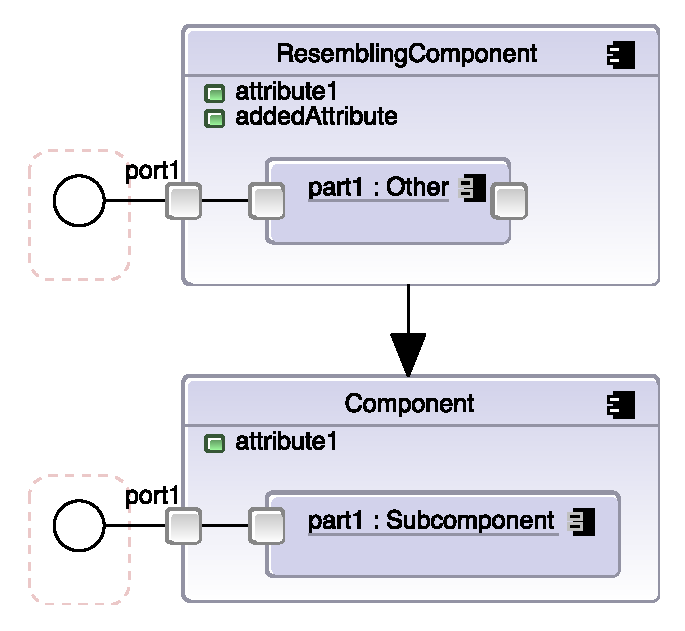
\includegraphics[width=0.5\columnwidth]{images/core-resemblance}
\par\end{centering}

\protect\caption{\label{fig:Resemblance-between-two}Resemblance between two composite
components}


\end{figure}


The deltas are move obvious in the textual description below.
\begin{lyxcode}
\textbf{\small{}component}{\small{}~Component~\{}{\small \par}

{\small{}~~~~}\textbf{\small{}attributes}{\small{}:}{\small \par}

{\small{}~~~~~~~~attribute1;}{\small \par}

{\small{}~~~~}\textbf{\small{}ports}{\small{}:}{\small \par}

{\small{}~~~~~~~~port1;}{\small \par}

{\small{}~~~~}\textbf{\small{}parts}{\small{}:}{\small \par}

{\small{}~~~~~~~~part1:~Subcomponent;}{\small \par}

{\small{}~~~~}\textbf{\small{}connectors}{\small{}:}{\small \par}

{\small{}~~~~~~~~conn1~joins~port@part~to~port1;}{\small \par}

{\small{}\}}~\\
\textbf{\small{}}~\\
\textbf{\small{}component}{\small{}~ResemblingComponent}{\small \par}

{\small{}~~~~~}\textbf{\small{}resembles}{\small{}~Component~\{}{\small \par}

{\small{}~~~~}\textbf{\small{}attributes}{\small{}:}{\small \par}

{\small{}~~~~~~~~addedAttribute;}{\small \par}

{\small{}~~~~}\textbf{\small{}replace-parts}{\small{}:}{\small \par}

{\small{}~~~~~~~~part1~}\textbf{\small{}becomes}{\small{}~part1:~Other}{\small \par}

{\small{}\}}{\small \par}


\end{lyxcode}
Resemblance is a many to one relation to permit the merging of multiple
component definitions that may have arisen due to, for example, distributed
development. It might be of concern that if a sufficiently radical
delta is applied to a component then the new definition will bear
little or no resemblance, in the general sense, to the component definitions
from which it is derived. However, this is of more philosophical than
practical import as the primary intent of resemblance to record change
or evolution and we can find many examples in both engineering and
nature where things evolve dramatically from their original form.

Resemblance may also be applied to interfaces in which case the modified
constituents are operations. If a resemblance delta consists only
of additions then when applied to an interface, it defines a proper
subtype. The type inference and checking algorithm we have implemented
in our prototype tool Evolve takes full cognizance of this.


\subsubsection*{Stratum}

A stratum is a module that holds the definitions relating to an initial
(base) software architecture expressed as a composite component, or
definitions relating to an evolution (extension) of that architecture.
Each stratum records its dependent strata needed to assemble a system,
and the builder uses the current stratum and the transitive closure
of all strata that this stratum depends on. The computation of resemblance
in the context of the stratum dependency graph is addressed in the
next section.

In addition to being a unit of architectural definition and extension,
the stratum is the unit of sharing and ownership. Each stratum is
owned by a single party that has modification rights to it. We can
therefore use strata to model the ownership structure of an architecture
and map this onto a community of base and extension developers. Our
development tool Evolve and the Backbone runtime environment support
the import and export of strata for distributing extensions and subsets
of an architecture.

A stratum is also a unit of deployment in that its compiled version
together with associated component code can be sent to an end user
to extend their system in a similar fashion to Eclipse Plugins \cite{Gamma2003,Chatley2003}.

Figure \ref{fig:Two-strata,-packing} shows the graphical form, where
two strata package up the previously mentioned resemblance relationship.
Note that we are showing components as their iconical form, rather
than as fully expanded with all their constituents.

\begin{figure}[h]
\noindent \begin{centering}
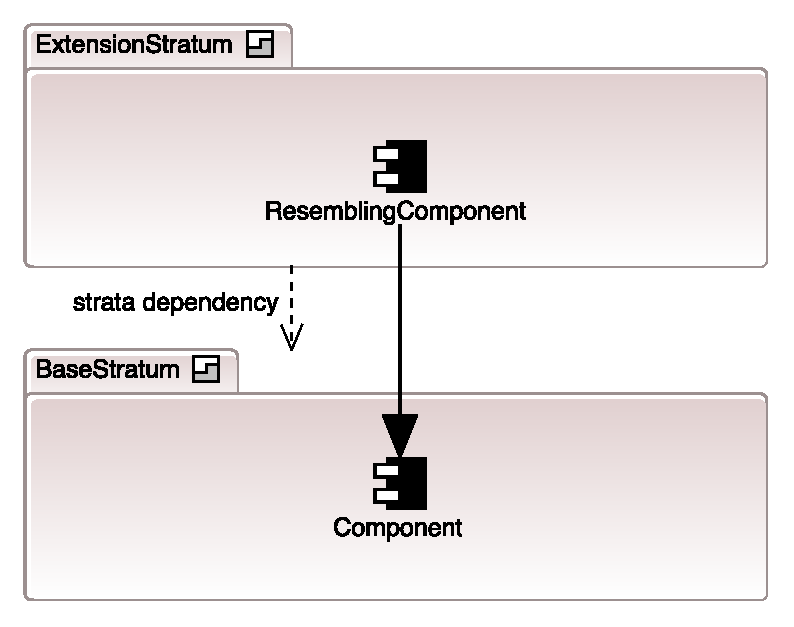
\includegraphics[width=0.6\columnwidth]{images/core-strata}
\par\end{centering}

\protect\caption{\label{fig:Two-strata,-packing}Two strata, packaging up a base architecture
and an extension}


\end{figure}



\subsubsection*{Replacement}

Replacement globally substitutes the definition of one component for
another, making sure that any use relations that referred to the original
definition will now refer to the replacement.

When we combine replacement and resemblance, we get evolution which
permits the incremental evolution of a component definition without
having to change the composite component definitions that use the
original component. We similarly combine the graphical notations of
resemblance and replacement to show that \texttt{Component`} incrementally
modifies \texttt{Component} and replaces it, in the context of stratum
\texttt{ExtensionStratum}.

We show the graphical form in figure \ref{fig:Resemblance-and-Replacement}.

\begin{figure}[h]
\noindent \begin{centering}
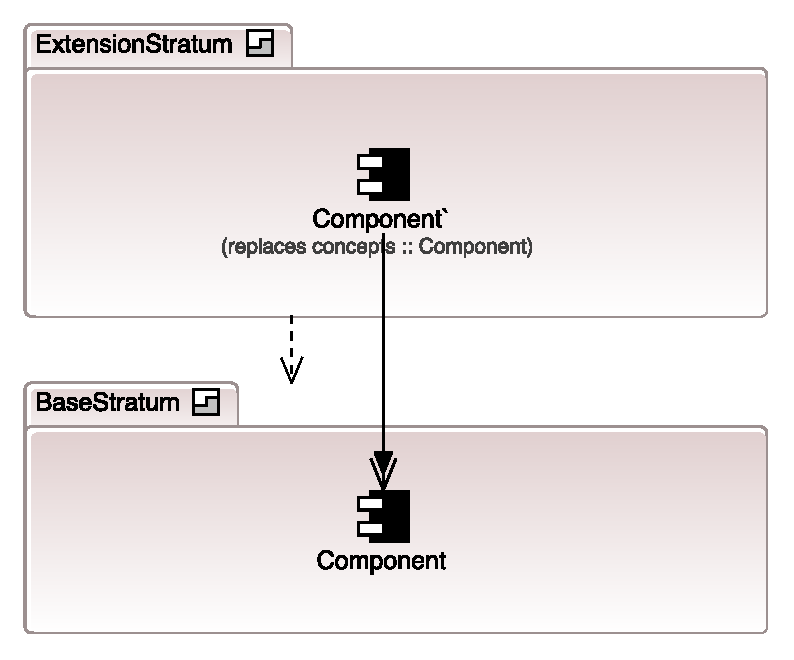
\includegraphics[width=0.6\columnwidth]{images/core-evolution}
\par\end{centering}

\protect\caption{\label{fig:Resemblance-and-Replacement}Resemblance and Replacement
combine to allow evolution}


\end{figure}


Textually, the separation of resemblance and replacement is clear.

\begin{minipage}[t]{1\columnwidth}%
\begin{lyxcode}
\textbf{\small{}~}~\\
\textbf{\small{}component}{\small{}~Component'}~\\
{\small{}~~~~~}\textbf{\small{}resembles}{\small{}~Component}~\\
{\small{}~~~~~}\textbf{\small{}replaces}{\small{}~Component~\{~...}~\\
{\small{}~}~\\
{\small \par}\end{lyxcode}
%
\end{minipage}

It is of course possible to resemble a different component from the
one being replaced, but it is usual for there to be at least an indirect
resemblance relationship in that case.

Components and interfaces in the Backbone ADL are given globally unique
identifiers to permit the correct unambiguous application of replacement.
Replacement is the key to managing change in composite hierarchical
definitions since it permits substitution of component definitions
at one level of the composition hierarchy without necessarily affecting
higher layers.

It should be noted that although evolution permits constituents to
be deleted in forming a new definition from existing defintions, this
is not destructive editing in the usual sense since the existing definition
is preserved and the deletion simply recorded in a delta in a different
stratum. Our approach preserves definitions and at no point overwrites
old definitions with new ones. We do not remove the base definition
but simply record the delta definition in the extension stratum. Even
retirement is modeled in this non-destructive way - if we do not want
a component definition to be available for use in an extension, we
simply replace it with an evolution that sets its retirement status
to true.

As a strata is a unit of architectural definition and ownership, it
does not make sense to have both a component and its replacement in
the same stratum. If the owner wished to evolve that component, they
could do it by simply modifying the definition, which they own. The
same is not true of resemblance though - a stratum may package both
a component and components which resemble it.


\subsection{Example}

To illustrate the use of these three concepts we use the Single Lane
Bridge example from \cite{McVeigh2011}. This concurrent system models
the access of cars to a single lane bridge. Its component architecture
can be modeled in Backbone as shown in figure \ref{fig:SingleLaneBridge-components}.

\begin{figure}[h]
\noindent \begin{centering}
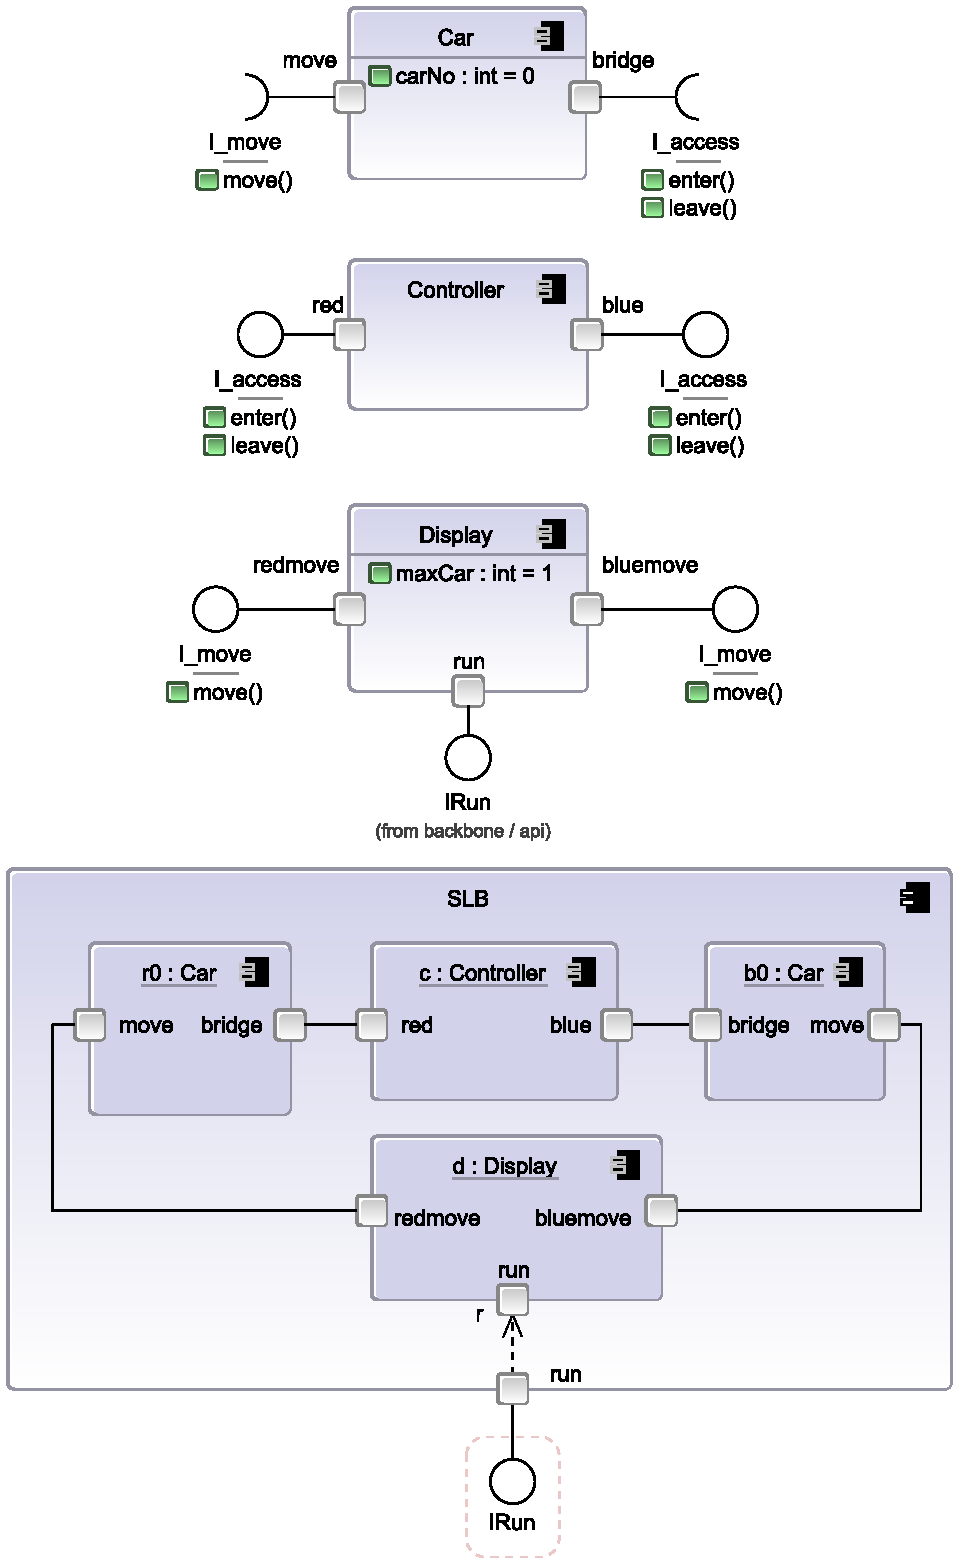
\includegraphics[scale=0.6]{images/slb-components}
\par\end{centering}

\protect\caption{\label{fig:SingleLaneBridge-components}SingleLaneBridge components}
\end{figure}


The textual architecture description that corresponds to this component
diagram is listed below:
\begin{lyxcode}
\textbf{\small{}stratum}{\small{}~Single\_Lane\_Bridge}{\small \par}

{\small{}~~}\textbf{\small{}depends-on}{\small{}~backbone}{\small \par}

{\small{}\{}{\small \par}

{\small{}~~~~}\textbf{\small{}interface}{\small{}~I\_access}{\small \par}

{\small{}~~~~~~}\textbf{\small{}implementation-class}{\small{}~bridge.I\_access}{\small \par}

{\small{}~~~~\{}{\small \par}

{\small{}~~~~~~}\textbf{\small{}operations:}{\small \par}

{\small{}~~~~~~~~enter;~leave;}{\small \par}

{\small{}~~~~\}}{\small \par}

{\small{}~~~~}\textbf{\small{}interface}{\small{}~I\_move}{\small \par}

{\small{}~~~~~~}\textbf{\small{}implementation-class}{\small{}~bridge.I\_move}{\small \par}

{\small{}~~~~\{}{\small \par}

{\small{}~~~~~~}\textbf{\small{}operations:}{\small \par}

{\small{}~~~~~~~~move;}{\small \par}

{\small{}~~~~\}}{\small \par}

{\small{}~~~~}\textbf{\small{}component}{\small{}~Controller}{\small \par}

{\small{}~~~~~~}\textbf{\small{}implementation-class}{\small{}~bridge.Controller}{\small \par}

{\small{}~~~~\{}{\small \par}

{\small{}~~~~~~}\textbf{\small{}ports:}{\small \par}

{\small{}~~~~~~~~red~}\textbf{\small{}provides}{\small{}~I\_access,}{\small \par}

{\small{}~~~~~~~~blue~}\textbf{\small{}provides}{\small{}~I\_access;}{\small \par}

{\small{}~~~~\}}{\small \par}

{\small{}~~~~}\textbf{\small{}component}{\small{}~Car}{\small \par}

{\small{}~~~~~~}\textbf{\small{}implementation-class}{\small{}~bridge.Car}{\small \par}

{\small{}~~~~\{}{\small \par}

{\small{}~~~~~~}\textbf{\small{}attributes:}{\small \par}

{\small{}~~~~~~~~carNo:~int~=~0;}{\small \par}

{\small{}~~~~~~}\textbf{\small{}ports:}{\small \par}

{\small{}~~~~~~~~move~}\textbf{\small{}requires}{\small{}~I\_move,}{\small \par}

{\small{}~~~~~~~~bridge~}\textbf{\small{}requires}{\small{}~I\_access;}{\small \par}

{\small{}~~~~\}}{\small \par}

{\small{}~~~~}\textbf{\small{}component}{\small{}~Display}{\small \par}

{\small{}~~~~~~}\textbf{\small{}implementation-class}{\small{}~bridge.Display}{\small \par}

{\small{}~~~~\{}{\small \par}

{\small{}~~~~~~}\textbf{\small{}attributes:}{\small \par}

{\small{}~~~~~~~~maxCar:~int~=~1;}{\small \par}

{\small{}~~~~~~}\textbf{\small{}ports:}{\small \par}

{\small{}~~~~~~~~redmove~}\textbf{\small{}provides}{\small{}~I\_move,}{\small \par}

{\small{}~~~~~~~~bluemove~}\textbf{\small{}provides}{\small{}~I\_move,}{\small \par}

{\small{}~~~~~~~~run~}\textbf{\small{}provides}{\small{}~IRun;}{\small \par}

{\small{}~~~~\}}{\small \par}

{\small{}~~~~}\textbf{\small{}component}{\small{}~SLB}{\small \par}

{\small{}~~~~\{}{\small \par}

{\small{}~~~~~~}\textbf{\small{}ports:}{\small \par}

{\small{}~~~~~~~~run~}\textbf{\small{}provides}{\small{}~IRun;}{\small \par}

{\small{}~~~~~~}\textbf{\small{}parts:}{\small \par}

{\small{}~~~~~~~~b0:~Car,}{\small \par}

{\small{}~~~~~~~~c:~Controller,}{\small \par}

{\small{}~~~~~~~~r0:~Car,}{\small \par}

{\small{}~~~~~~~~d:~Display;}{\small \par}

{\small{}~~~~~~}\textbf{\small{}connectors:}{\small \par}

{\small{}~~~~~~~~bb~}\textbf{\small{}joins}{\small{}~blue@c~}\textbf{\small{}to}{\small{}~bridge@b0,}{\small \par}

{\small{}~~~~~~~~br~}\textbf{\small{}joins}{\small{}~bridge@r0~}\textbf{\small{}to}{\small{}~red@c,}{\small \par}

{\small{}~~~~~~~~vr~}\textbf{\small{}joins}{\small{}~move@r0~}\textbf{\small{}to}{\small{}~redmove@d,}{\small \par}

{\small{}~~~~~~~~vb~}\textbf{\small{}joins}{\small{}~move@b0~}\textbf{\small{}to}{\small{}~bluemove@d,}{\small \par}

{\small{}~~~~~~~~r~}\textbf{\small{}delegates-from}{\small{}~run~}\textbf{\small{}to}{\small{}~run@d;}{\small \par}

{\small{}~~~~\}}{\small \par}

{\small{}\}}{\small \par}
\end{lyxcode}
This architecture represents a system with one red car and one blue
car, moving in opposite directions, competing for access to the bridge.
Access control is implemented by the Controller component, which provides
two I\_access interfaces. A Car calls enter to gain access to the
bridge and calls leave on exit. Cars display their movement using
the Display component. Note that all of the definitions are contained
in the SingleLaneBridge stratum that appears in Figure \ref{fig:SingleLaneBridge-components}.
Car, Controller and Display are leaf components with an implementaion
defined by Java classes. SLB is a composite component that contains
parts made from these components interconnected by connectors to form
the system.


\subsubsection*{Using Resemblance}

Now suppose that another developer wishes to evolve this system to
accommodate multiple red and blue cars moving in opposite directions.
This developer creates the stratum with the components shown in figure
\ref{fig:MultiCarBridge-components}. The developer defines three
new components: CarFactory dynamically creates a Car component when
it receives an invocation on its creator port, CarCreator is a leaf
component that calls its create port maxCar times, and finally, the
composite component MultiCar creates nCars Car components.

\begin{figure}[h]
\noindent \begin{centering}
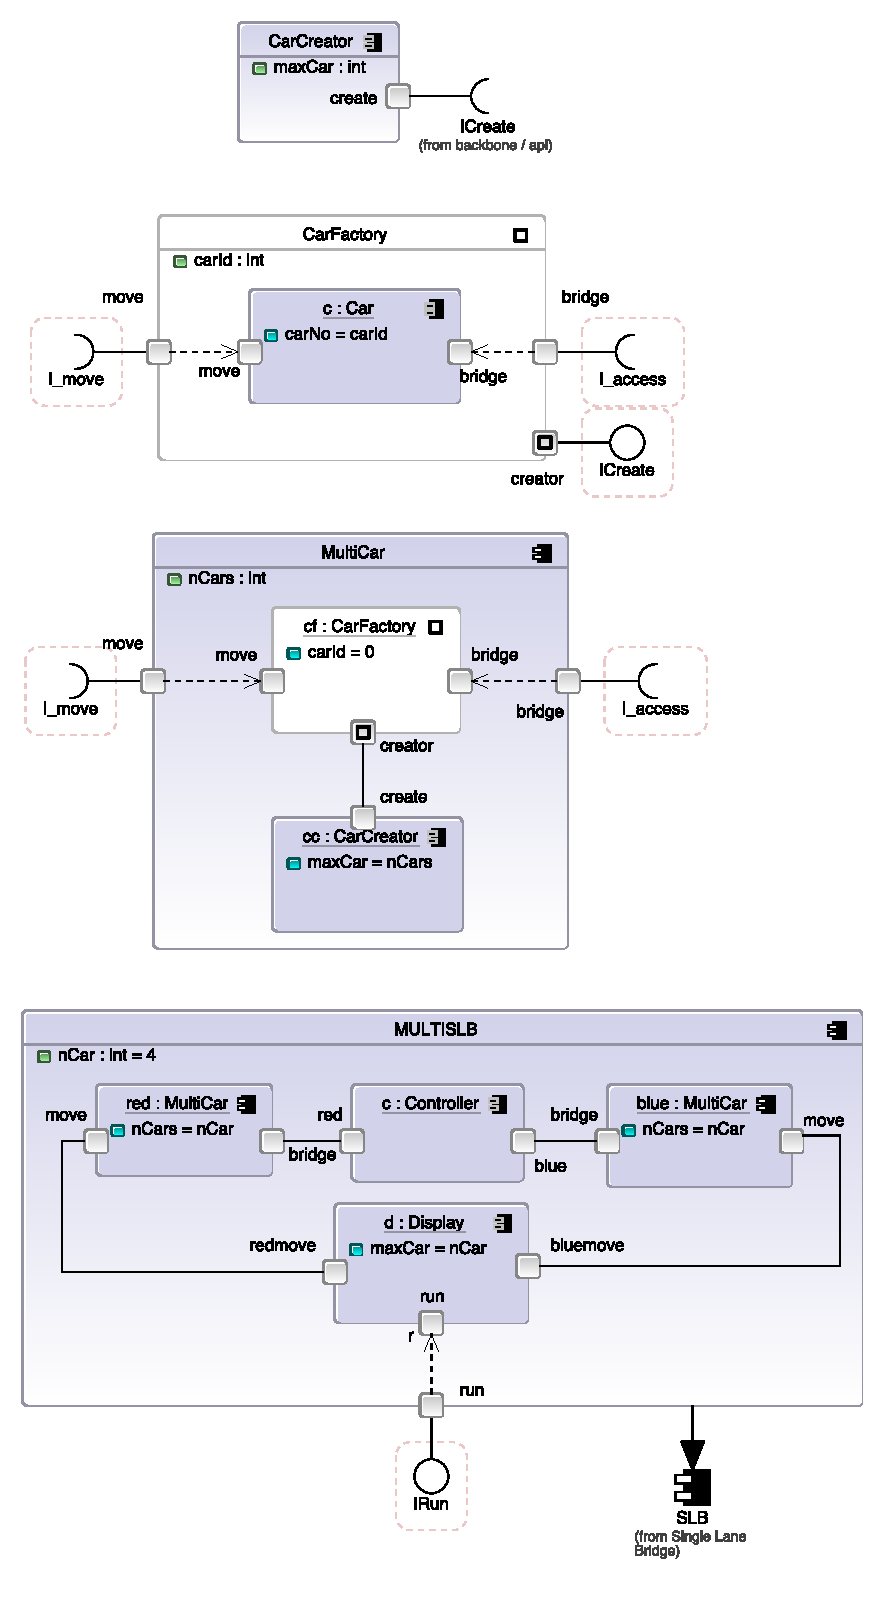
\includegraphics[scale=0.6]{images/mlb-components}
\par\end{centering}

\protect\caption{\label{fig:MultiCarBridge-components}MultiCarBridge components}


\end{figure}




The MULTSLB composite component is defined as a resemblance of the
SLB component from the SingleLaneBridge stratum. Graphically, resemblance
is depicted as a solid arrow pointing to an icon representing the
component from which the resemblance is derived. Although graphically
MULTSLB is depicted with all its component parts and connectors, in
fact as shown in the Backbone listing below, it is defined by a delta
that simply adds the nCar attribute and replaces the parts of type
Car with parts of type MultiCar. In addition, it replaces the instance
of Display with an instance of the same component type but with a
different attribute value. The new definition is formed graphically
by editing the previous definition that the Evolve tool displays when
the resemblance relation is established.
\begin{lyxcode}
\textbf{\small{}stratum}{\small{}~Multi\_Car\_Bridge}{\small \par}

{\small{}~~}\textbf{\small{}depends-on}{\small{}~Single\_Lane\_Bridge}{\small \par}

{\small{}\{}{\small \par}

{\small{}~~~~}\textbf{\small{}component}{\small{}~CarFactory~is-factory}{\small \par}

{\small{}~~~~~~~}\textbf{\small{}resembles}{\small{}~FactoryBase}{\small \par}

{\small{}~~~~\{}{\small \par}

{\small{}~~~~~~}\textbf{\small{}attributes:}{\small \par}

{\small{}~~~~~~~~~~carId:~int;}{\small \par}

{\small{}~~~~~~}\textbf{\small{}ports:}{\small \par}

{\small{}~~~~~~~~~~bridge,}{\small \par}

{\small{}~~~~~~~~~~move;}{\small \par}

{\small{}~~~~~~}\textbf{\small{}parts:}{\small \par}

{\small{}~~~~~~~~~~c:~Single\_Lane\_Bridge::Car}{\small \par}

{\small{}~~~~~~~~~~~~~~~}\textbf{\small{}slots:}{\small \par}

{\small{}~~~~~~~~~~~~~~~~~carNo~=~carId;}{\small \par}

{\small{}~~~~~~}\textbf{\small{}connectors:}{\small \par}

{\small{}~~~~~~~~~~b~}\textbf{\small{}delegates-from}{\small{}~move~}\textbf{\small{}to}{\small{}~move@c,}{\small \par}

{\small{}~~~~~~~~~~m~}\textbf{\small{}delegates-from}{\small{}~bridge~}\textbf{\small{}to}{\small{}~bridge@c;}{\small \par}

{\small{}~~~~\}}{\small \par}

{\small{}~~~~}\textbf{\small{}component}{\small{}~CarCreator}{\small \par}

{\small{}~~~~~~}\textbf{\small{}implementation-class}{\small{}~bridge.CarCreator}{\small \par}

{\small{}~~~~\{}{\small \par}

{\small{}~~~~~~}\textbf{\small{}attributes:}{\small \par}

{\small{}~~~~~~~~maxCar:~int;}{\small \par}

{\small{}~~~~~~}\textbf{\small{}ports:}{\small \par}

{\small{}~~~~~~~~create~requires~ICreate;}{\small \par}

{\small{}~~~~\}}{\small \par}

{\small{}~~~~}\textbf{\small{}component}{\small{}~MultiCar}{\small \par}

{\small{}~~~~\{}{\small \par}

{\small{}~~~~~~}\textbf{\small{}attributes:}{\small \par}

{\small{}~~~~~~~~nCars:~int;}{\small \par}

{\small{}~~~~~}\textbf{\small{}~ports:}{\small \par}

{\small{}~~~~~~~~bridge,}{\small \par}

{\small{}~~~~~~~~move;}{\small \par}

{\small{}~~~~~~}\textbf{\small{}parts:}{\small \par}

{\small{}~~~~~~~~cc:~CarCreator}{\small \par}

{\small{}~~~~~~~~~~}\textbf{\small{}slots:}{\small \par}

{\small{}~~~~~~~~~~~~maxCar~=~nCars,}{\small \par}

{\small{}~~~~~~~~cf:~CarFactory}{\small \par}

{\small{}~~~~~~~~~~}\textbf{\small{}slots:}{\small \par}

{\small{}~~~~~~~~~~~~carId~=~0;}{\small \par}

{\small{}~~~~~}\textbf{\small{}~connectors:}{\small \par}

{\small{}~~~~~~~~c~}\textbf{\small{}joins}{\small{}~create@cc~}\textbf{\small{}to}{\small{}~creator@cf,}{\small \par}

{\small{}~~~~~~~~b~}\textbf{\small{}delegates-from}{\small{}~bridge~}\textbf{\small{}to}{\small{}~bridge@cf,}{\small \par}

{\small{}~~~~~~~~m~}\textbf{\small{}delegates-from}{\small{}~move~}\textbf{\small{}to}{\small{}~move@cf;}{\small \par}

{\small{}~~~~\}}{\small \par}

{\small{}~~~~}\textbf{\small{}component}{\small{}~MULTISLB}{\small \par}

{\small{}~~~~~~}\textbf{\small{}resembles}{\small{}~Single\_Lane\_Bridge::SLB}{\small \par}

{\small{}~~~~\{}{\small \par}

{\small{}~~~~~~}\textbf{\small{}attributes:}{\small \par}

{\small{}~~~~~~~~nCar:~int~=~4;}{\small \par}

{\small{}~~~~~~}\textbf{\small{}replace-parts:}{\small \par}

{\small{}~~~~~~~~r0~}\textbf{\small{}becomes}{\small{}~red:~MultiCar}{\small \par}

{\small{}~~~~~~~~~~}\textbf{\small{}slots:}{\small \par}

{\small{}~~~~~~~~~~~~nCars~=~nCar}{\small \par}

{\small{}~~~~~~~~~~}\textbf{\small{}port-remaps:}{\small \par}

{\small{}~~~~~~~~~~~~move~}\textbf{\small{}maps-onto}{\small{}~xxx}{\small \par}

{\small{}~~~~~~~~~~~~bridge~}\textbf{\small{}maps-onto}{\small{}~xxx,}{\small \par}

{\small{}~~~~~~~~b0~}\textbf{\small{}becomes}{\small{}~blue:~MultiCar}{\small \par}

{\small{}~~~~~~~~~~}\textbf{\small{}slots:}{\small \par}

{\small{}~~~~~~~~~~~~nCars~=~nCar}{\small \par}

{\small{}~~~~~~~~~~}\textbf{\small{}port-remaps:}{\small \par}

{\small{}~~~~~~~~~~~~move~}\textbf{\small{}maps-onto}{\small{}~xxx}{\small \par}

{\small{}~~~~~~~~~~~~bridge~}\textbf{\small{}maps-onto}{\small{}~xxx,}{\small \par}

{\small{}~~~~~~~~d~}\textbf{\small{}becomes}{\small{}~d:~Single\_Lane\_Bridge::Display}{\small \par}

{\small{}~~~~~~~~~~}\textbf{\small{}slots:}{\small \par}

{\small{}~~~~~~~~~~~~maxCar~=~nCar;}{\small \par}

{\small{}~~~~\}}{\small \par}

{\small{}\}}{\small \par}
\end{lyxcode}
To produce this extension permitting multiple cars, some new program
source code must be written to implement the CarCreator component,
however, there is no requirement to access or modify any of the source
code relating to the base SingleLaneBridge stratum. Access to the
architecture description is sufficient to permit extension. Note that
resemblance is also used to define CarFactory, which extends FactoryBase
provided by the underlying backbone stratum. The stratum dependency
graph for the extension is shown in Figure \ref{fig:MultiCarBridge-strata-dependency}.

\begin{figure}[h]
\noindent \begin{centering}
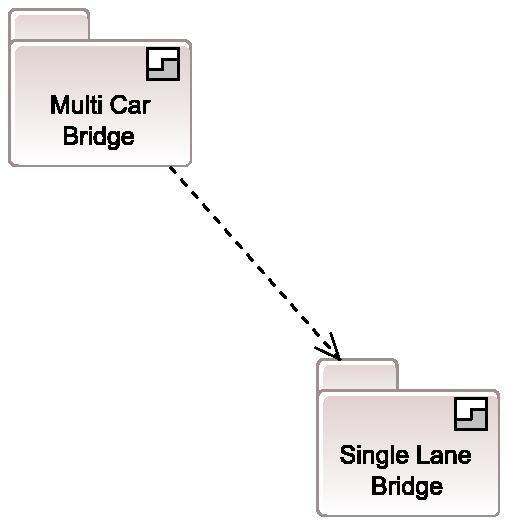
\includegraphics[width=0.4\columnwidth]{images/multicar-stratum}
\par\end{centering}

\protect\caption{\label{fig:MultiCarBridge-strata-dependency}MultiCarBridge strata
dependency graph}


\end{figure}



\subsubsection*{Using Replacement}

The single lane bridge Controller component works well until the number
of cars increases to the point that a stream of cars, either red of
blue, continuously occupies the bridge denying access to cars moving
in the other direction. In other words, the Controller component is
safe but not fair. Figure \ref{fig:FairBridge-replacement-controlle}
shows how a revised Controller that does implement fairness is introduced.

\begin{figure}[h]
\noindent \begin{centering}
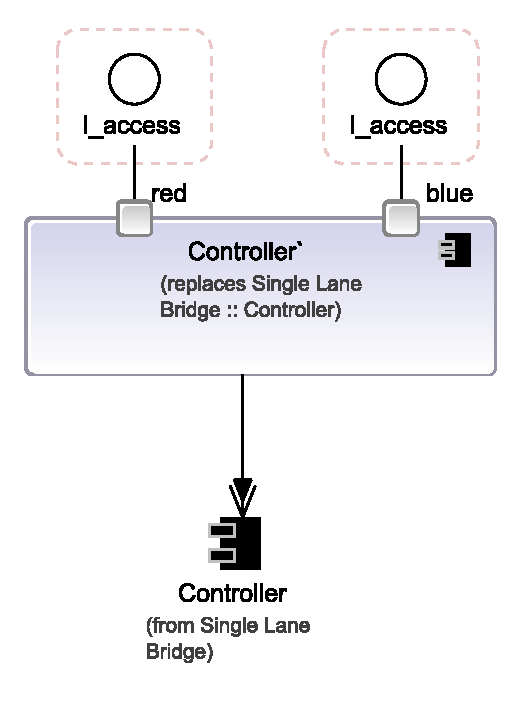
\includegraphics[width=0.35\columnwidth]{images/fair-controller}
\par\end{centering}

\protect\caption{\label{fig:FairBridge-replacement-controlle}FairBridge replacement
controller}
\end{figure}


The listing below shows the Backbone textual represenation of the
evolved controller.

{\small{}}%
\begin{minipage}[t]{1\columnwidth}%
\begin{lyxcode}
\textbf{\small{}~}~\\
\textbf{\small{}stratum}{\small{}~Fair\_Bridge}{\small \par}

{\small{}~}\textbf{\small{}depends-on}{\small{}~Single\_Lane\_Bridge}{\small \par}

{\small{}\{}{\small \par}

{\small{}~}\textbf{\small{}component~}{\small{}Controller}{\small \par}

{\small{}~~}\textbf{\small{}implementation-class}{\small \par}

{\small{}~~~~bridge.FairController}{\small \par}

{\small{}~~}\textbf{\small{}resembles}{\small \par}

{\small{}~~~~Single\_Lane\_Bridge::Controller}{\small \par}

{\small{}~}\textbf{\small{}~replaces}{\small \par}

{\small{}~~~~Single\_Lane\_Bridge::Controller}{\small \par}

{\small{}~~\{}{\small \par}

{\small{}~~\}}{\small \par}

{\small{}\}}{\small \par}

~~\\
\end{lyxcode}
%
\end{minipage}{\small \par}

Replacement is so often combined with resemblance that we use a single
graphical symbol (combined solid and fishbone arrow) to indicate this
combination as shown in figure \ref{fig:FairBridge-replacement-controlle}.
The diagram and text show that we are replacing Controller with a
component that resembles it exactly with the exception of the implementation
class that we have changed. We can now combine this fair bridge controller
with the MultiCarBridge stratum as shown in Figure 5. The stratum
FairMultiCarBridge represents a system that permits multiple cars
and has a fair controller. The stratum contains no definitions of
components or deltas; it simply indicates its dependences as shown
in the Backbone text below Figure \ref{fig:FairMultiLaneBridge-strata-depen}.

\begin{figure}[h]
\noindent \begin{centering}
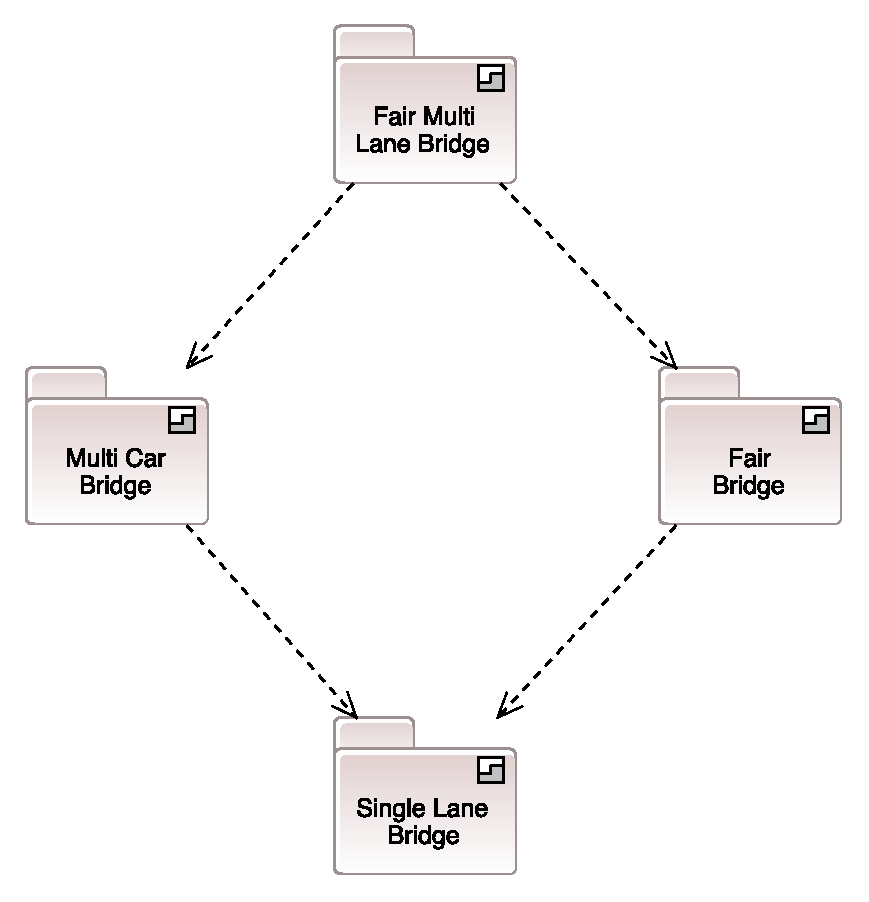
\includegraphics[width=0.7\columnwidth]{images/all-strata}
\par\end{centering}

\protect\caption{\label{fig:FairMultiLaneBridge-strata-depen}FairMultiLaneBridge strata
dependency graph}
\end{figure}

\begin{lyxcode}
\textbf{\small{}stratum}{\small{}~Fair\_Multi\_Lane\_Bridge}{\small \par}

{\small{}~~}\textbf{\small{}depends-on~}{\small{}Multi\_Car\_Bridge,~Fair\_Bridge}{\small \par}

{\small{}\{}{\small \par}

{\small{}\}}{\small \par}


\end{lyxcode}
Figure \ref{fig:FairMultiLaneBridge-strata-depen} illustrates how
strata are merged. This can of course lead to conflicts in definitions,
which we discuss in the next section. In the case of the example,
a more plausible scenario would be for the original base developer,
or a third party, to export this new stratum to the multi-car developer
who could import it as shown in Figure \ref{fig:Alternative-dependency-graph}.
If we were to write out the Backbone text again, it would now show
a dependency on FairBridge rather than SingleLaneBridge for MultiCarBridge.
\begin{figure}[h]
\noindent \begin{centering}
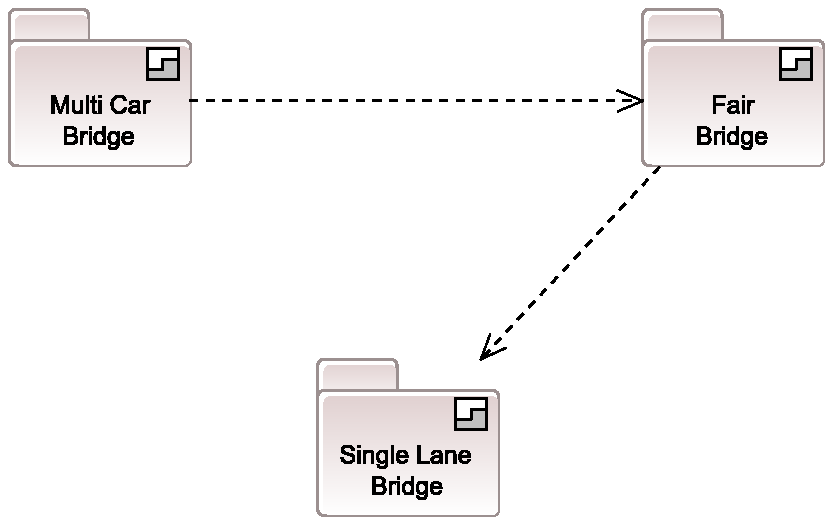
\includegraphics[width=0.7\columnwidth]{images/alternative-graph}
\par\end{centering}

\protect\caption{\label{fig:Alternative-dependency-graph}Alternative dependency graph}


\end{figure}



\section{\label{sec:A-Formal-Description}A Formal Description of Backbone}

In this section we formally describe how components, defined in an
extension stratum using a combination of resemblance and replacement,
can evolve the existing compositional structure of an architecture
defined in a base stratum.

The ability to evolve an architecture in a decentralized manner, where
strata are used to group and organise these component definitions,
leads naturally to the desire to combine and merge strata that each
evolve a common base into a unified architecture. We describe the
merging rules, showing that any structural errors can be corrected
by adding further component definitions.

To make the treatment more concrete we present a variant of our bridge
system (figure \ref{fig:A-variant-of}) and demonstrate how the formal
model applies to this architecture. We have (\texttt{MULTISLB} resembles
\texttt{SLB}), (\texttt{SLBa\textquoteright{}} evolves \texttt{SLB})
and (\texttt{SLBb\textquoteright{}} evolves \texttt{SLB}). In other
words, the three middle strata represent branches of the original
system. The top stratum has visibility of all branches and hence merges
these, bringing the definitions into one place with potential conflicts.

\begin{figure}[h]
\noindent \begin{centering}
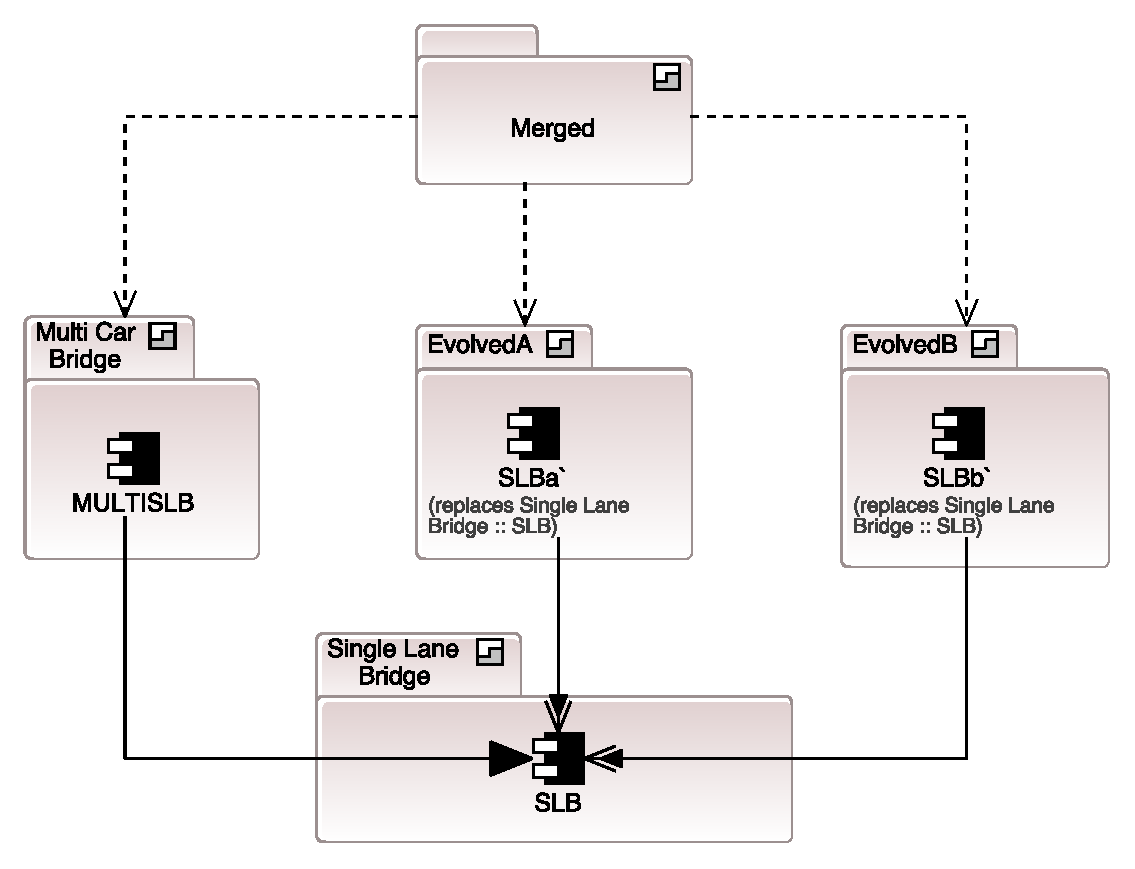
\includegraphics[width=0.8\columnwidth]{images/formal-merged}
\par\end{centering}

\protect\caption{\label{fig:A-variant-of}A variant of the Bridge system}


\end{figure}


The formal model is specified in Alloy \cite{Jackson2006,Jackson2002},
which is a relational logic supported by model checking tools. The
full specification is presented in the appendix at the end of this
report. Dependencies between strata in an extension architecture govern
the order of application of resemblance and replacement. We therefore
begin by describing the stratum concept.


\subsection{Structures}
\begin{lyxlist}{00.00.0000}
\item [{\emph{Definition}}] A \emph{stratum} is a hierarchical module that
owns and groups elements (component and interface) definitions.
\end{lyxlist}
A stratum may depend on a set of other strata and it owns a set of
elements. An element is an abstraction of a component or interface
or other compositional artifact. We model stratum as below.
\begin{lyxcode}
{\footnotesize{}sig~Stratum~\{}{\footnotesize \par}

{\footnotesize{}~~dependson:~set~Stratum,}{\footnotesize \par}

{\footnotesize{}~~elements:~set~Element,}{\footnotesize \par}

{\footnotesize{}~~...~\}}{\footnotesize \par}
\end{lyxcode}
Transitive strata dependencies determine which other elements are
visible to elements in that stratum for use in composition, resemblance
and replacement relationships.

We outlaw circular dependencies between strata, forcing the structure
into a graph.
\begin{lyxcode}
{\footnotesize{}all~s:~Stratum~|~s~not~in~s.\textasciicircum{}dependson}{\footnotesize \par}
\end{lyxcode}
This allows us to divide strata into those a given stratum depends
on (transitively), those that depend on it, and those it has no visibility
of.

Two strata are termed independent if they have no visibility of each
other. If independent strata depend on common underlying strata, like
\texttt{EvolvedA} and \texttt{EvolvedB} in figure X, we call them
branches.
\begin{lyxcode}
{\footnotesize{}pred~branch{[}a,~b:~Stratum{]}~\{}{\footnotesize \par}

{\footnotesize{}~~let~alla~=~a.{*}dependson,~allb~=~b.{*}dependson~|}{\footnotesize \par}

{\footnotesize{}~~~~a~not~in~allb~and~b~not~in~alla~and}{\footnotesize \par}

{\footnotesize{}~~~~~~some~alla~\&~allb}{\footnotesize \par}

{\footnotesize{}\}}{\footnotesize \par}\end{lyxcode}
\begin{lyxlist}{00.00.0000}
\item [{\emph{Definition}}] An \emph{element} is a compositional structure,
such as a component or interface, that can participate in resemblance
and replacement relationships.
\end{lyxlist}
It is represented by the following structure.
\begin{lyxcode}
{\footnotesize{}sig~Element~\{}{\footnotesize \par}

{\footnotesize{}~~home:~Stratum,}{\footnotesize \par}

{\footnotesize{}~~resembles:~set~Element,}{\footnotesize \par}

{\footnotesize{}~~replaces:~lone~Element,}{\footnotesize \par}

{\footnotesize{}~~deltas:~lone~Deltas}{\footnotesize \par}

{\footnotesize{}\}}{\footnotesize \par}
\end{lyxcode}
Each element has a single home stratum, which owns it, in accord with
the \texttt{Stratum::elements} set. An element can resemble any number
of other elements of the same type that are visible to, or in, the
home stratum, and optionally replace an element from a stratum that
the home (transitively) depends upon.

As seen below, we disallow having both the initial definition of an
element and its replacement in the same home. This is because stratum
is a unit of solitary development ownership - if the owner (person
or group) of a stratum wished to adjust the structure of an owned
component, they would edit the definition directly rather than creating
a replacement. Element replacement conversely allows developers to
make adjustments to strata they do not have ownership of.
\begin{lyxcode}
{\footnotesize{}all~e:~Element~|}{\footnotesize \par}

{\footnotesize{}~~~~let~res~=~e.resembles,~rep~=~e.replaces~|}{\footnotesize \par}

{\footnotesize{}~~res.home~in~e.home.{*}dependson}{\footnotesize \par}

{\footnotesize{}~~~~and~rep.home~in~e.home.\textasciicircum{}dependson}{\footnotesize \par}

{\footnotesize{}~~~~and~e~not~in~res~}{\footnotesize \par}\end{lyxcode}
\begin{lyxlist}{00.00.0000}
\item [{\emph{Definition}}] A \emph{deltas} structure holds the adds, deletes
or replacements to the resembled constituent structure of an element\footnote{There are two types of replacement in Backbone: element replacement
where one element can be substituted for another, and delta replacement
where an element definition replaces some of the constituents that
have been inherited via resemblance. Here we are talking about the
latter concept.}
\end{lyxlist}
We model deltas as shown. Note that a constituent is a building block
of an element. In the case of a component, this could be a port, a
connector, an attribute or a part. Other than having an identity,
constituent in our specification is just a placeholder.
\begin{lyxcode}
{\footnotesize{}sig~Deltas~\{}{\footnotesize \par}

{\footnotesize{}~~owner:~Element,}{\footnotesize \par}

{\footnotesize{}~~add,~delete:~set~Constituent,}{\footnotesize \par}

{\footnotesize{}~~replace:~Constituent~->~Constituent}{\footnotesize \par}

{\footnotesize{}\}}{\footnotesize \par}
\end{lyxcode}
The \texttt{add} and \texttt{delete} fields indicate constituents
to add or delete. The \texttt{replace} field is a relation fom the
constituent being replaced to that replacing it. A key point is that
any replacing constituent assumes the identity of the replaced one
- this allows connectors and other references to the replaced item
to stay valid.

If an element does not resemble another then all the deltas will be
adds which build up the initial structure.


\subsection{The Expanded Resemblance Graph}
\begin{lyxlist}{00.00.0000}
\item [{\emph{Definition}}] The \emph{expanded resemblance graph} is a
resemblance graph for a given element from a given stratum perspective,
which takes into account any replacements visible from that perspective.
\end{lyxlist}
The expanded resemblance graph is the resemblance graph for an element
after all the replacements from extension strata have been factored
in.

Consider, for example, that the \texttt{MULTISLB} non-expanded resemblance
graph is (\texttt{MULTISLB} resembles \texttt{SLB}). If we compute
the expanded resemblance graph from the perspective of \texttt{Merged},
then we need to take into account that two additional replacements
(evolutions) are present. From this perspective, the expanded resemblance
graph would now look like (\texttt{MULTISLB} resembles \texttt{SLBa\textquoteright{}}
+ \texttt{SLBb\textquoteright }, \texttt{SLBa\textquoteright{}} resembles
\texttt{SLB}, \texttt{SLBb\textquoteright{}} resembles \texttt{SLB}).
This is shown graphically in figure \ref{fig:The-expanded-resemblance}.

\begin{figure}[h]
\noindent \begin{centering}
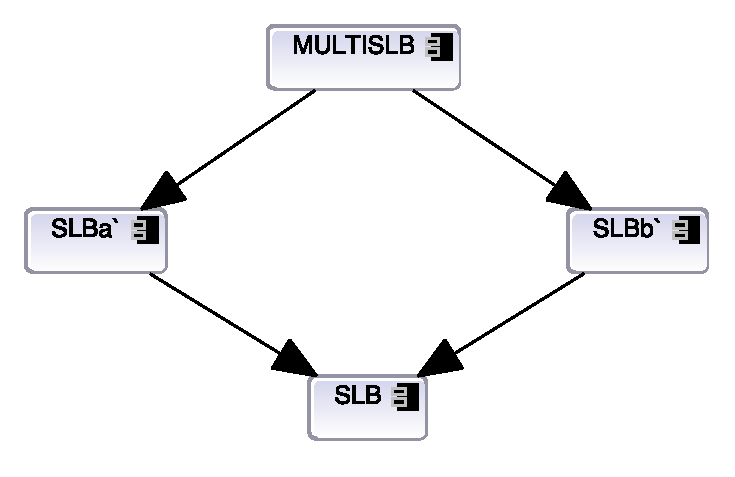
\includegraphics[width=0.6\columnwidth]{images/formal-expanded}
\par\end{centering}

\protect\caption{\label{fig:The-expanded-resemblance}The expanded resemblance graph
for \texttt{MULTISLB}}


\end{figure}


From the same perspective, consider that \texttt{SLB} has a two headed
expanded resemblance graph, reflecting that \texttt{SLBa\textquoteright{}}
and \texttt{SLBb\textquoteright{}} have no direct visibility of each
other. If these definitions conflict then any issues could be corrected
by a new evolution in the \texttt{Merged} stratum which could add,
delete or replace constituents to ensure well formedness. Similarly,
it may be the case from the \texttt{Merged} perspective that evolutions
to \texttt{SLB} invalidate the \texttt{MULTISLB} definition. Again,
any issues can be rectified using evolutions in \texttt{Merged}. For
instance, if we have both an evolution of \texttt{SLB} to correct
the merged definition, and a further evolution to \texttt{MULTISLB}
then the expanded graph for \texttt{MULTISLB} would look as shown
in figure \ref{fig:Correcting-any-compositional}.

\begin{figure}[h]
\noindent \begin{centering}
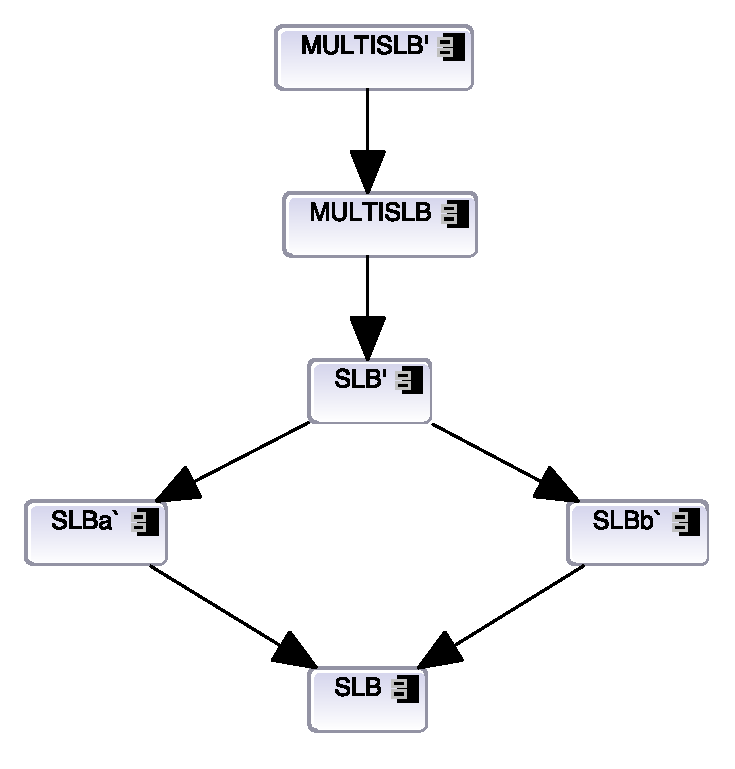
\includegraphics[width=0.6\columnwidth]{images/formal-corrected}
\par\end{centering}

\protect\caption{\label{fig:Correcting-any-compositional}Correcting any compositional
conflicts}


\end{figure}


The expanded graph is at the heart of our extension approach. In a
nutshell, replacement in an extension stratum allows us to insert
elements into an existing resemblance graph without directly editing
existing definitions. We can use replacement to effect changes to
compositional structure or to correct conflicts caused when we merge
branches.

The expanded graph specification relies on a notion of the topmost
definition of an element for a given perspective. In our original
example, from the \texttt{Single Lane Bridge} perspective, the topmost
definition of \texttt{SLB} is simply \texttt{SLB}. However, from the
perspective of \texttt{Merged} it is the set (\texttt{SLBa\textquoteright },
\texttt{SLBb\textquoteright }). To hold the topmost and expanded graph
information we add the following field to the \texttt{Stratum} structure:
\begin{lyxcode}
{\footnotesize{}sig~Stratum~\{}{\footnotesize \par}

{\footnotesize{}~~...}{\footnotesize \par}

{\footnotesize{}~~topmost:~Element~->~Element,}{\footnotesize \par}

{\footnotesize{}~~eresembles:~Element~->~Element,}{\footnotesize \par}

{\footnotesize{}~~...}{\footnotesize \par}

{\footnotesize{}\}}{\footnotesize \par}
\end{lyxcode}
\texttt{Topmost} is determined in the following way, where \texttt{s}
is the stratum perspective.
\begin{lyxcode}
{\footnotesize{}all~s:~Stratum,~e:~Element~\{}{\footnotesize \par}

{\footnotesize{}~~...}{\footnotesize \par}

{\footnotesize{}~~let~reps~=~replaces.e~\&~s.elements~|}{\footnotesize \par}

{\footnotesize{}~~~~some~reps~=>~s.topmost{[}e{]}~=~reps}{\footnotesize \par}

{\footnotesize{}~~~~~~else}{\footnotesize \par}

{\footnotesize{}~~~~e.home~=~s~=>~s.topmost{[}e{]}~=~e}{\footnotesize \par}

{\footnotesize{}~~~~~~else}{\footnotesize \par}

{\footnotesize{}~~~~s.topmost{[}e{]}~=~s.dependson.topmost{[}e{]}}{\footnotesize \par}

{\footnotesize{}~~...~}{\footnotesize \par}

{\footnotesize{}\}}{\footnotesize \par}
\end{lyxcode}
The first condition determines whether or not there is a replacement
of element \texttt{e} in \texttt{s}. If so, this is clearly the topmost
definition. Otherwise, if the perspective is the same as the element\textquoteright s
home stratum, then the topmost is simply the original element. Finally,
if none of these situations hold then we defer recursively to the
strata that the perspective depends upon\footnote{The \texttt{topmost} field and definition are effectively defining
a recursive function.}.

We can now compute \texttt{eresembles}, the expanded graph, using
the following logic.
\begin{lyxcode}
{\footnotesize{}let~joint~=~e.resembles~\&~ee.}{\footnotesize \par}

{\footnotesize{}~~~~replaces,rest~=~e.resembles~-~joint~|}{\footnotesize \par}

{\footnotesize{}~~s.eresembles{[}e{]}~=}{\footnotesize \par}

{\footnotesize{}~~~~e.home.dependson.topmost{[}joint{]}}{\footnotesize \par}

{\footnotesize{}~~~~+~s.topmost{[}rest{]}}{\footnotesize \par}
\end{lyxcode}
The \texttt{joint} set contains any elements that \texttt{e} is evolving
- i.e. where replacement and resemblance overlap. If we have evolution,
we need to look not at the current stratum (where \texttt{topmost}
would erroneously pick up the element \texttt{e} as a replacement),
but instead at the next lowest down strata in the dependency graph.
For all other resembled elements we can start at the current stratum.
It is also worth noting that for any replacement relation, the target
is the original unevolved element, even if another evolution of the
same element is visible to us underneath our home strata. This way,
even if we move the strata dependencies around we will not invalidate
any evolutions.


\subsection{Applying Deltas}

We are now in a position to apply the deltas by walking up the expanded
resemblance graph and adding, deleting and replacing constituents.
To hold the accumulated deltas we add the following fields to the
\texttt{Stratum} structure:
\begin{lyxcode}
{\footnotesize{}sig~Stratum~\{}{\footnotesize \par}

{\footnotesize{}~~...}{\footnotesize \par}

{\footnotesize{}~~edeltas:~Element~->~lone~Deltas,}{\footnotesize \par}

{\footnotesize{}~~full:~Element~->~Constituent~->~Constituent}{\footnotesize \par}

{\footnotesize{}\}}{\footnotesize \par}
\end{lyxcode}
For a given perspective \texttt{s}, element \texttt{e}, the deltas
from the expanded graph are accumulated into the \texttt{edeltas}
field as follows:
\begin{lyxcode}
{\footnotesize{}all~s:~Stratum,~e:~Element~\{}{\footnotesize \par}

{\footnotesize{}~~let~lower~=~s.eresembles{[}e{]},}{\footnotesize \par}

{\footnotesize{}~~~~~~me~=~s.edeltas{[}e{]}}{\footnotesize \par}

{\footnotesize{}~~\{}{\footnotesize \par}

{\footnotesize{}~~~~me.add~=~s.edeltas{[}lower{]}.add~+~e.deltas.add}{\footnotesize \par}

{\footnotesize{}~~~~me.delete~=~s.edeltas{[}lower{]}.delete}{\footnotesize \par}

{\footnotesize{}~~~~~~+~e.deltas.delete}{\footnotesize \par}

{\footnotesize{}~~~~me.replace~=~s.edeltas{[}lower{]}.replace}{\footnotesize \par}

{\footnotesize{}~~~~~~++~e.deltas.replace}{\footnotesize \par}

{\footnotesize{}~~~\}}{\footnotesize \par}

{\footnotesize{}\}}{\footnotesize \par}
\end{lyxcode}
In the above, we start with the element \texttt{e} from the perspective
\texttt{s}. We get the elements (\texttt{lower}) that \texttt{e} resembles
in the expanded graph. Then we form a new \texttt{Deltas} structure
(\texttt{edeltas}) by recursively summing up the deltas of the lower
elements and the deltas element of \texttt{e} itself - we union adds
and deletes and overwrite the lower replaces with the element\textquoteright s
replaces.

Finally, we form the complete structure (\texttt{full}) by finding
all topmost definitions of a given element \texttt{e}, and combining
the constituents by applying additions, replacements and finally deletions.
This order of application means that if one branch deletes a constituent
and another replaces it, then the deletion will always win out.
\begin{lyxcode}
{\footnotesize{}all~s:~Stratum,~e:~Element~\{}{\footnotesize \par}

{\footnotesize{}~~let~tops~=~s.topmost{[}e{]},~me~=~s.edeltas{[}tops{]}~|}{\footnotesize \par}

{\footnotesize{}~~~~some~e.replaces~=>~no~s.full{[}e{]}}{\footnotesize \par}

{\footnotesize{}~~~~~~else}{\footnotesize \par}

{\footnotesize{}~~~~s.full{[}e{]}~=}{\footnotesize \par}

{\footnotesize{}~~~~~~\{~a,~b:~me.add~|~a~=~b~\}}{\footnotesize \par}

{\footnotesize{}~~~~~~++~me.replace}{\footnotesize \par}

{\footnotesize{}~~~~~~-~\{~d:~me.delete,~allds:~Constituent~\}}{\footnotesize \par}

{\footnotesize{}\}}{\footnotesize \par}
\end{lyxcode}
The field \texttt{full} is actually a relation (\texttt{Constituent
- > Constituent}), reflecting that even if we replace a constituent
(right hand side) it still retains the identity of the original constituent
(left hand side). As described, this allows existing connectors to
stay valid. An addition of constituent \texttt{X} will result in an
\texttt{X -> X} entry.

The ability to express changes as deltas allows a component to completely
remake its inherited structure using a combination of adds, deletes
and replaces. Combined with the ability to remake an element\textquoteright s
resemblance graph using extension strata, an extension can adjust
the architecture of a system in any way it pleases without destructively
editing the original definition.


\subsection{Structural Conflicts}

Structural conflict occurs when two branches make incompatible evolutions
to the same element, and we then merge them into a common stratum.
For instance, \texttt{SLBa\textquoteright{}} might replace constituent
\texttt{X} with \texttt{Y} and \texttt{SLBb\textquoteright{}} might
replace \texttt{X} with \texttt{Z}. Upon merge, we retain both replacements,
and the full structure contains (\texttt{X -> Y}, and \texttt{X ->
Z}). When the \texttt{full} set of relations is not a partial function,
this type of conflict has occured- i.e. when we have more than one
range value for the same domain value in the set of relations.
\begin{lyxcode}
{\footnotesize{}pred~conflict{[}perspective:~Stratum,~e:~Element{]}~\{}{\footnotesize \par}

{\footnotesize{}~~not~functional{[}~perspective.full{[}e{]},~Element~{]}}{\footnotesize \par}

{\footnotesize{}\}}{\footnotesize \par}
\end{lyxcode}
This dilemma can be rectified by a subsequent evolution which definitively
replaces the constituent, say (\texttt{X -> Q}). This will overwrite
(\texttt{++}) all the previous entries that have \texttt{X} as the
domain value, as per the delta application rules.

More subtle conflicts occur when the adjusted structure in a branch
is compositionally incompatible with assumptions made in another branch.
For instance, one branch might delete a connector which the other
branch was relying on to be present. An expanded variant of the above
formal specification detects this by describing the actual component
model in terms of parts, ports, connectors and attributes rather than
generic constituents, and expressing well-formedness rules \cite{McVeigh2009}.


\subsubsection{Implementation of the Specification}

The Java runtime engine implementation of Backbone is based on the
expanded specification mentioned above, which additionally covers
areas such as the full component model, port type inference and interface
subtype rules. Of particular interest is the use of UUIDs to represent
element and constituent identity. Concretely, each constituent is
allocated a unique identifier, and when a constituent replaces this
it assumes the UUID of the replaced constituent. In the above specification
we have relied on direct element identity instead.


\subsubsection{Summary}

The formal specification explains how an extension stratum can affect
the resemblance graph of an existing element in an architecture. It
also details the rules via which delta application occurs, leading
to the full structure from a given stratum perspective. These rules
allow an extension stratum to control the way in which deltas of existing
elements are applied, allowing it to make any changes to the original
architecture required to support the extension.

\begin{comment}
\bibliographystyle{plain}
\bibliography{\string"/Users/amcveigh/Personal/evolve/Academic Work/read papers/references\string"}
\end{comment}




\section{Intrinsic Definition in Practice}

Proposers of a new approach to software architecture description have
the responsibility to demonstrate that it can be put into industrial
practice. In this section, we discuss three significant barriers to
doing so and outline how they are addressed. They are: tool support,
compatibility with existing libraries and toolkits, and application
to existing legacy software. The first two issues are addressed in
this section, and the applicability to legacy and mature software
is addressed in section \ref{sec:Applicability-to-Mature}.


\subsection{Tool Support}

The Backbone ADL is supported by a graphical modeling tool Evolve,
and a runtime environment which instantiates and interconnects components
from a Backbone description. Figure \ref{fig:The-DeltaEngine-is}
is an overview of the elements that make up the modeling tool and
runtime environment. The DeltaEngine layer implements the algorithm
described in the previous section and is used in both the modeling
tool to build graphical representations of composite components from
delta definitions and also in the runtime environment to instantiate
components from these same definitions. In addition to this interpreted
runtime the modeling tool can optionally compile a \textquotedblleft flat\textquotedblright{}
description of the model as a builder class. In this case, no runtime
environment is required. It should be noted that even the interpreted
runtime environment incurs no overhead during execution of a system;
it is only active at startup time when it directs instantiation and
interconnection.

\begin{figure}[h]
\noindent \begin{centering}
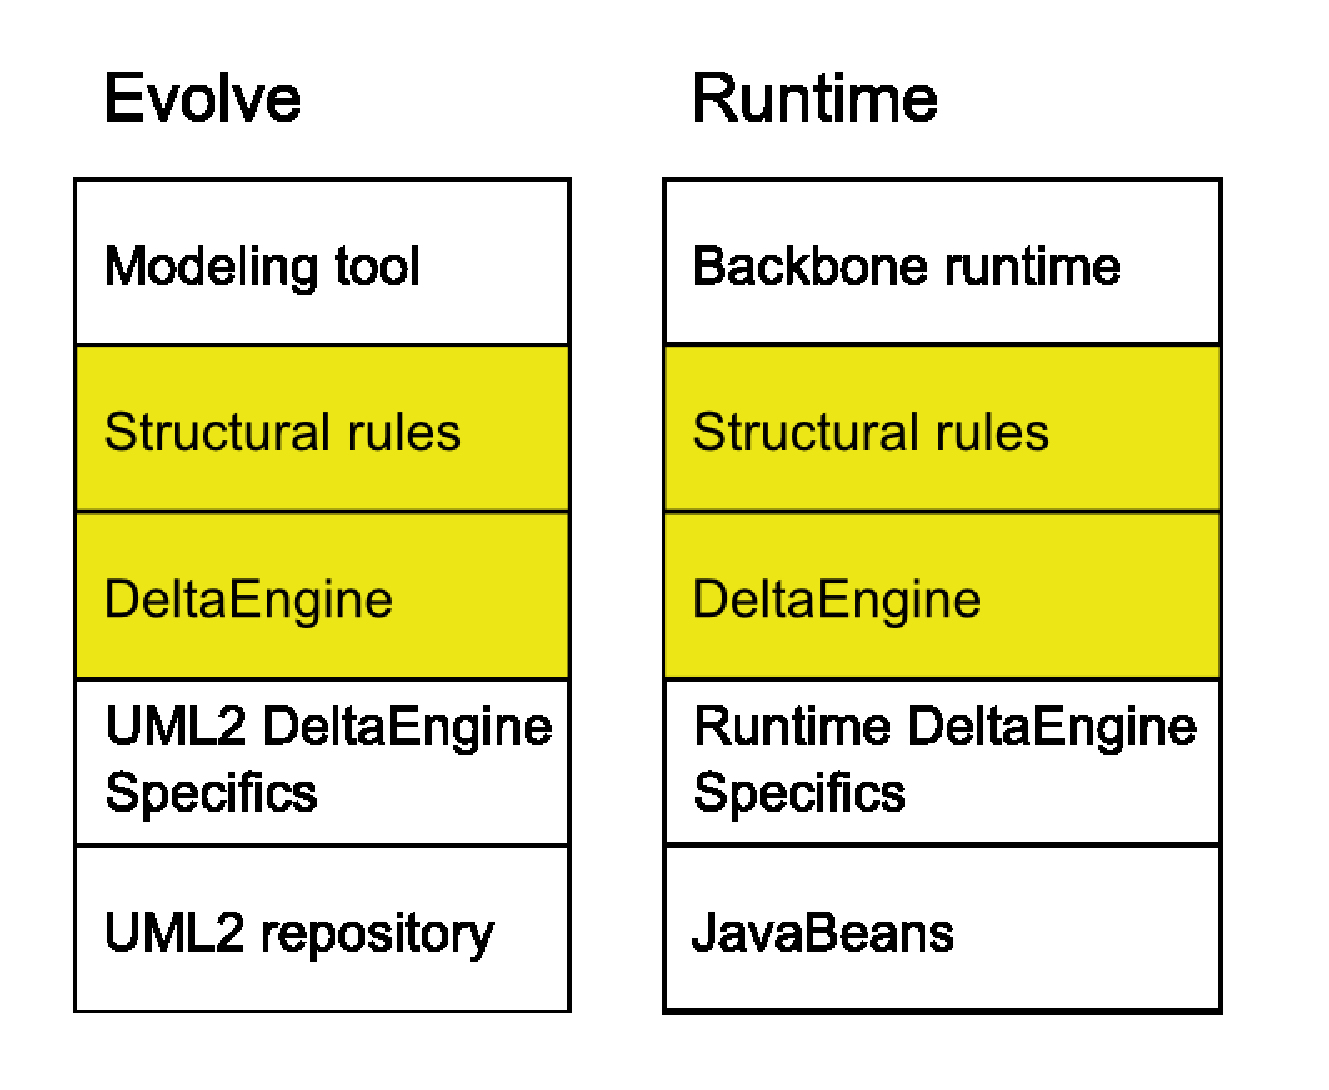
\includegraphics[width=0.6\columnwidth]{drawings/stack}
\par\end{centering}

\protect\caption{\label{fig:The-DeltaEngine-is}Common layers between environments}
\end{figure}



\subsubsection{The DeltaEngine and Structural Rules Layers}

The DeltaEngine layer is a library which implements the extended resemblance
algorithm described in section \ref{sec:A-Formal-Description} allowing
deltas to be applied in the correct order to fully realise each component.
Once the deltas are applied, the Structural rules layer can be used
to determine if the system is structurally well-formed using 100+
rules \cite{McVeigh2009}. Any errors are catalogued against the elements
responsible.


\subsubsection{Evolve Graphical Modeling Environment}

\begin{figure}[h]
\noindent \begin{centering}
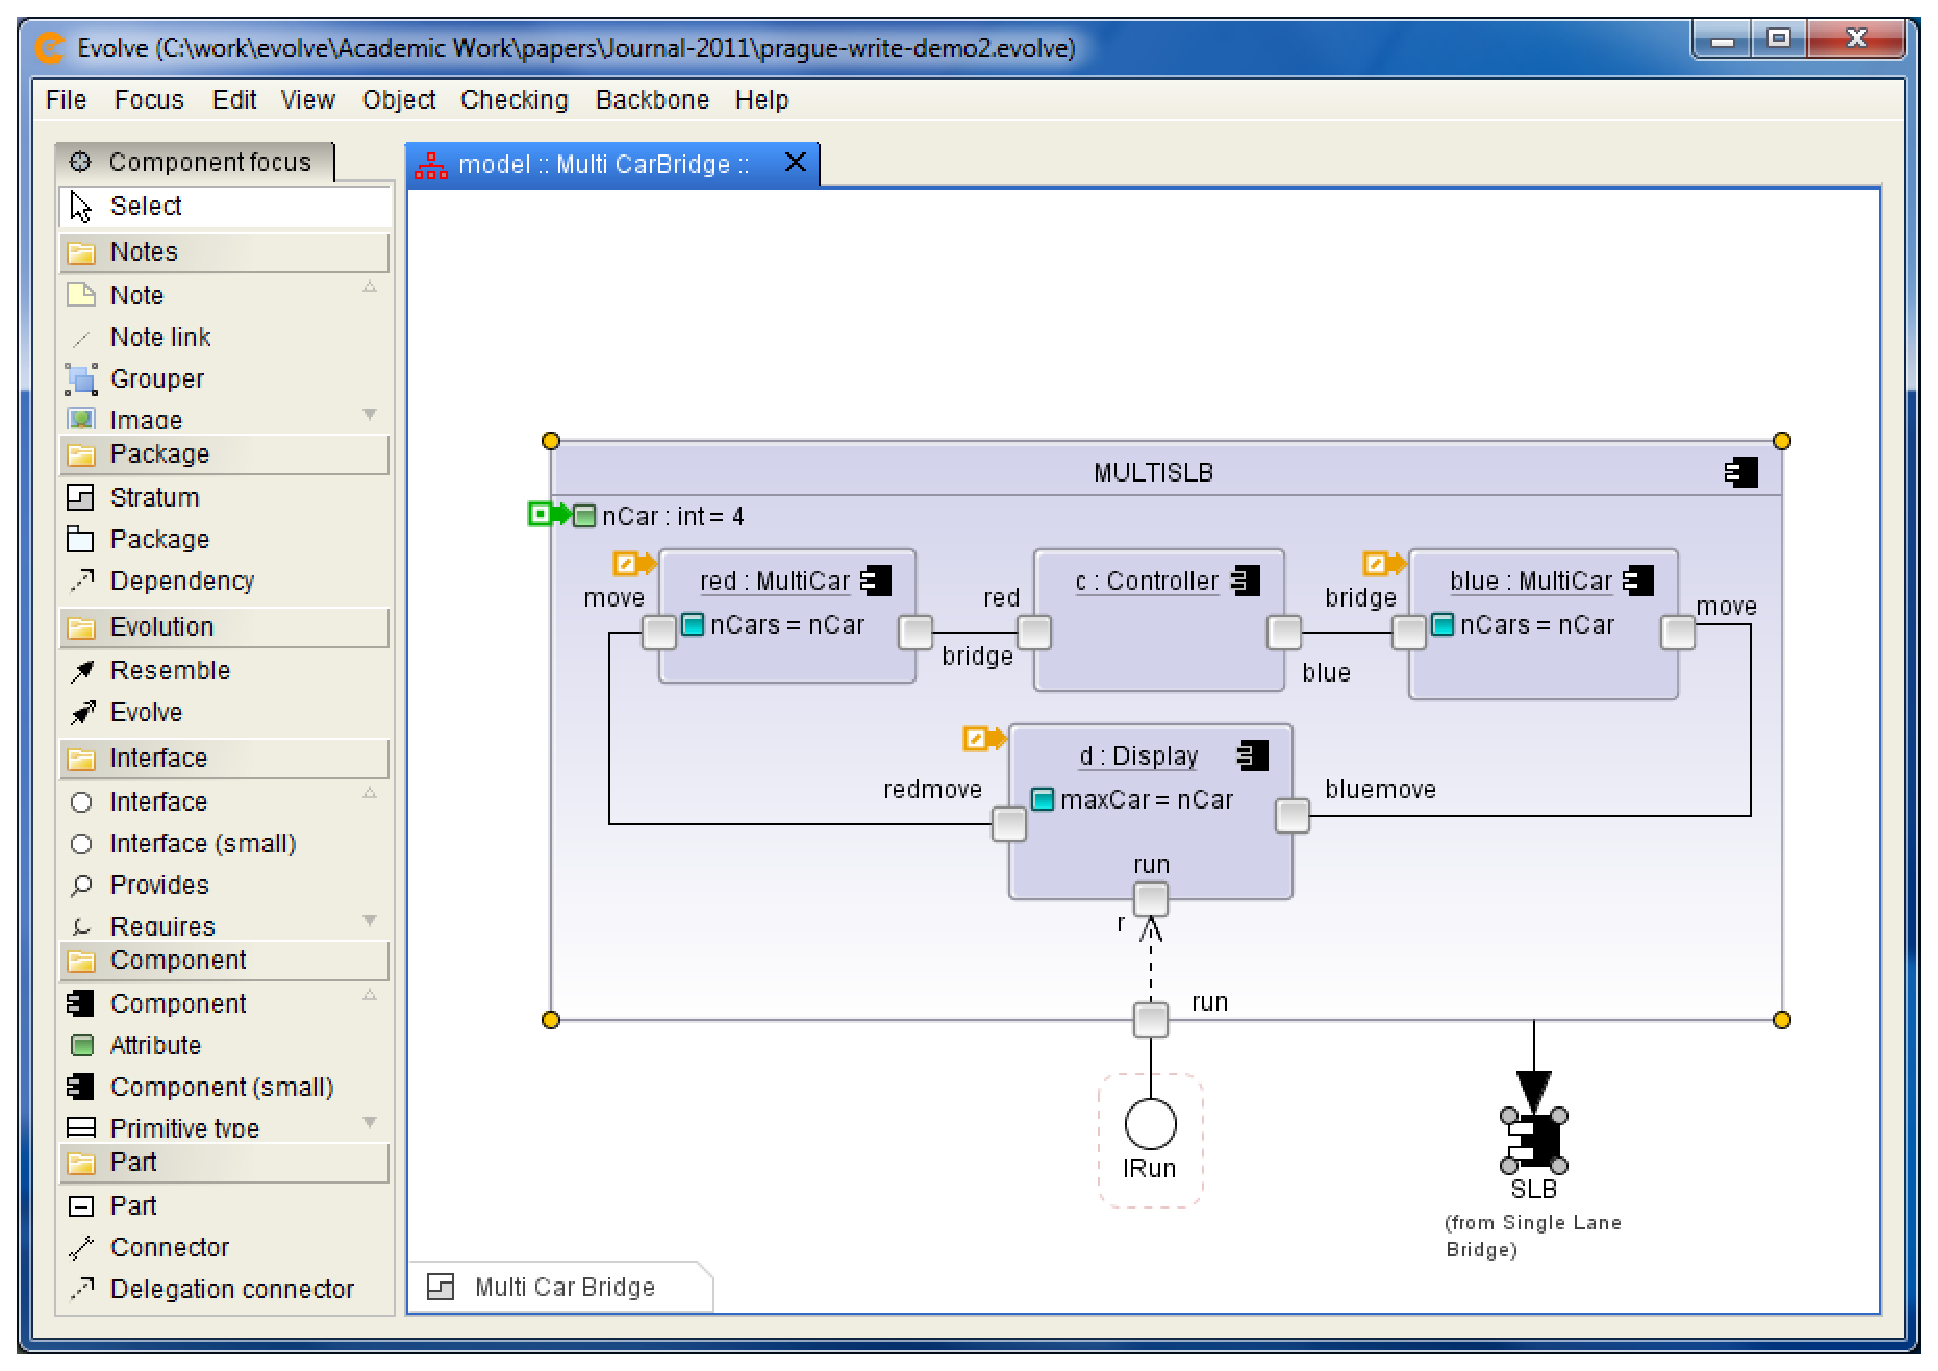
\includegraphics[width=0.5\paperwidth]{drawings/deltas}
\par\end{centering}

\protect\caption{\label{fig:Evolve-showing-deltas}Evolve showing deltas}
\end{figure}


Evolve uses standard UML2 component diagrams. We do however apply
both restrictions and extensions to this notation in order to better
match up to our component model. We implement the restrictions as
rules and the extensions as stereotypes as per the UML2 philosophy.
As an example consider that UML2 allows part multiplicity. Evolve
does not allow this feature, instead requiring the use of factory
components for multiple instantiation: this requires restriction preventing
the use of multiplicity and an extension to allow factory components
to be denoted by a stereotype. In total, however, the number of mismatches
between the two component models is quite small reflecting the historical
lineage of both Backbone and the UML2 component model in the models
that have preceded them \cite{Garlan1997,Selic1994a,Magee1995}.

It has been noted that a design tool must support both top-down and
bottom-up approaches in order to match up with the creative design
processes involved \cite{Taylor2010}. Evolve naturally supports bottom-up
composition by virtue of the compositional model chosen. To better
support top-down design we incorporate placeholder components \cite{Medvidovic1999}
which are components which are not yet fully elaborated, allowing
the designer to terminate top-down decomposition at an arbitrary point
rather than just at leaf components. Placeholders may have all the
features of a normal component, but may not be instantiated directly.
Any component can be marked as a placeholder.

Because resemblance and replacement can be used to substitute placeholder
components and parts, placeholders can participate fully in the design
process. For instance it is common in Evolve to have a placeholder
at the base of a resemblance hierarchy, effectively acting as a template
for the more refined components that derive from it.

Although Backbone requires that components are described in terms
of deltas, Evolve always shows the full structure even as it records
deltas for any changes. As shown in figure \ref{fig:Evolve-showing-deltas}
Evolve can overlay the deltas graphically on the expanded structures.


\subsubsection{Runtime}

The runtime inteprets the textual form emitted from Evolve - it is
effectively an interpreter for the Backbone structural domain specific
language \cite{McVeigh2006} at the heart of the system. It shares
the DeltaEngine and rules layers with Evolve, guaranteeing consistency
between the two environments. Instead of using the engine to display
graphical forms, the runtime uses the engine to apply the deltas to
form fully realised components, which have links back to the actual
implementation class via the implementation-class annotations. It
then flattens the hierarchy and uses reflection to instantiate and
connect up the instances in conformance to the architecture. At that
point control can be handed off to the leaf component presenting the
IRun interface which represents the starting point of the program.

Alternatively Evolve can emit code for a builder class representing
the flattened structure of the system - this requires no runtime and
has all facilities available including factory instantiation. This
mode is particularly useful in supported but constrained environments
such as the Google Web Toolkit \cite{GWT,GWT-Apps} which do not support
full reflection and other advanced virtual machine features.

Although nothing prevents support for other languages, currently the
runtime is targeted to the Java language and the Java virtual machine.
Reflection is used extensively in the implementation of the runtime,
but as noted previously this only adds overhead in the direct construction
of component instances. If a builder class is emitted instead of using
the runtime, then there is no overhead compared to a conventional
Java program.


\subsection{\label{sub:Compatibility-with-Existing}Compatibility with Existing
Libraries}

Java has a lightweight component model called JavaBeans \cite{Network2006,O'Neill1998}
which uses a set of lexical conventions to allow setting and getting
of properties on classes. Evolve allows bean libraries to be imported
and translated into full Backbone leaf components by considering any
implemented interfaces of a bean to be provided interfaces on a port
called \texttt{main}, and any settable properties that are interfaces
to be required interfaces. In this way existing Java libraries are
fully compatible with the Evolve approach, and can be connected up
into composite components. This is in contrast with the conventional
JavaBeans wiring approach which is oriented explicitly around events
and hence required interfaces only.

Figure \ref{fig:Imported-Swing-components} shows a number of well-known
Swing \cite{Hoy2002} components that have been imported into Evolve
for use in an application.

\begin{figure}[h]
\noindent \begin{centering}
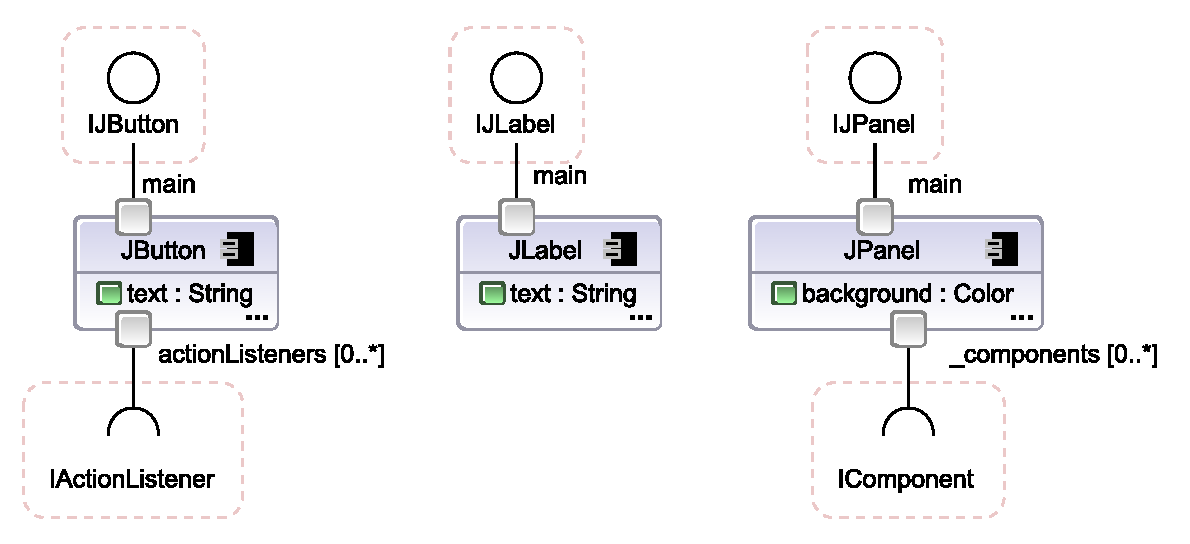
\includegraphics[width=1\columnwidth]{images/swing}
\par\end{centering}

\protect\caption{\label{fig:Imported-Swing-components}Imported Swing components}


\end{figure}



\section{\label{sec:Applicability-to-Mature}Applicability to Mature and Legacy
Systems}

To evaluate the applicability of the approach to existing software,
we chose to introduce our component model into the LTSA system \cite{Magee1999}
which was created by two of the authors previously for analysing the
properties of concurrent programs. Our intention was to model the
evolution of this mature system and to gain insights into the way
that evolution and architectural explication interact.

The original codebase is around 16k physical lines of code from over
200 classes. It consists of a graphical front end along with an automata-based
engine which can analyze the properties of finite state process expressions
using model checking.

LTSA has evolved into several variants over years, reflecting its
relatively wide use in academia and industry and the somewhat decentralized
nature of its development. We chose to concentrate on the original
system, the NASA-AMES evolution \cite{Giannakopoulou2003}, and a
separate evolution created for the exercise called DualWindow. Furthermore,
we wished to model the merged AMES and DualWindow systems.


\subsection{An Initial View of the Architecture}

We performed a first pass at forming a shallow and coarse-grained
compositional structure for the original LTSA application, reflecting
that it is not feasible to restructure a mature application in one
step. The intention was to demonstrate that the approach can be applied
with relatively small effort initially, with benefits accruing as
the system is incrementally decomposed further into smaller components
over time.

We started by spending some time understanding the LTSA code - for
this we used the primary author who was not familiar with the existing
system. After this a strata graph was formed and handful of top-level
candidate classes were identified for turning into components.

We refactored these classes into JavaBeans and imported them into
Evolve. Finally, a top-level composite called LTSA was created which
wired these together allowing the system to execute inside the Evolve
environment. This work took two person-days of effort in total.

The strata graph for the system is shown in figure \ref{fig:The-strata-for}.

\begin{figure}[h]
\noindent \begin{centering}
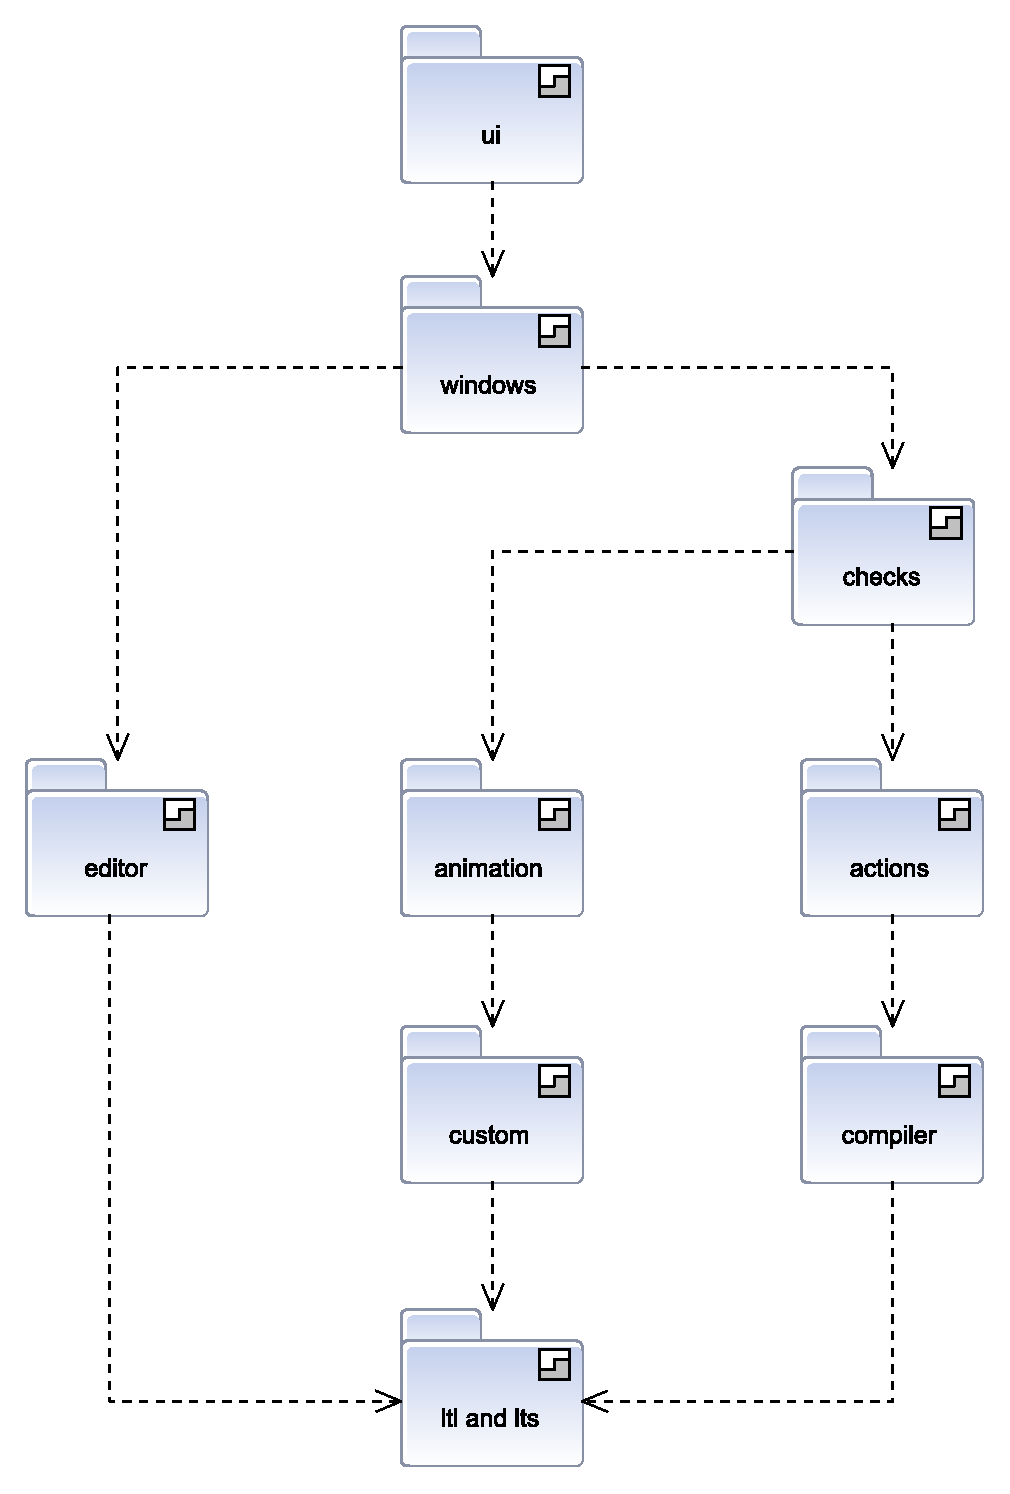
\includegraphics[width=0.7\columnwidth]{images/ltsa-strata}
\par\end{centering}

\protect\caption{\label{fig:The-strata-for}The strata for the LTSA application}


\end{figure}


As the architecture was now visible as components, further decomposition
was straight forward. After spending another day of modest refactoring
the refined compositional hierarchy in figure \ref{fig:LTSA-decompositions}
(B) was produced. Note that the original decomposition (A) was a subset
of this refinement - decomposing involves exposing further parts of
the architecture. At this point many of the features of the graphical
interface were exposed as components.

\begin{figure}[h]
\noindent \begin{centering}
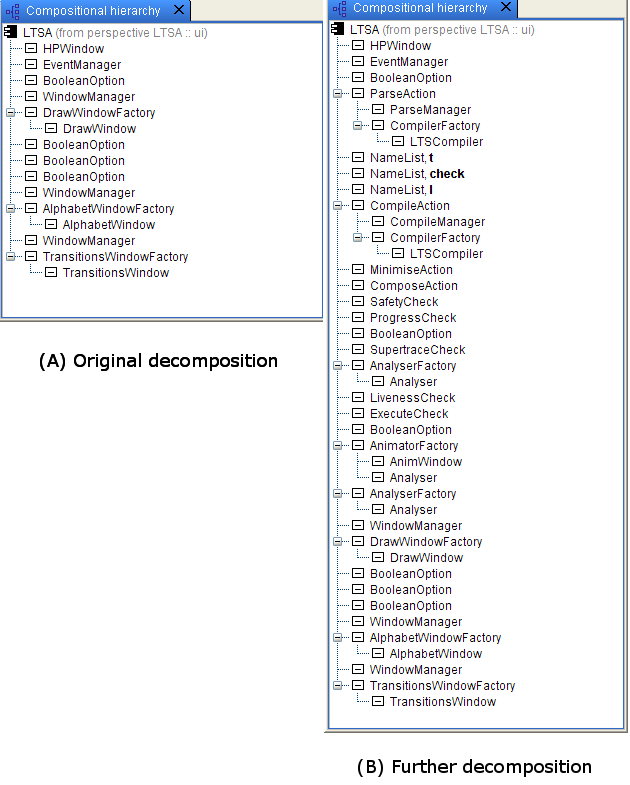
\includegraphics[width=0.8\columnwidth]{drawings/ltsa-initial-hierarchy}
\par\end{centering}

\protect\caption{\label{fig:LTSA-decompositions}LTSA decompositions}


\end{figure}


The top level LTSA component and the HPWindow component which managed
other windows looked as in figure \ref{fig:Top-level-LTSA} at this
point.

\begin{figure}[h]
\noindent \begin{centering}
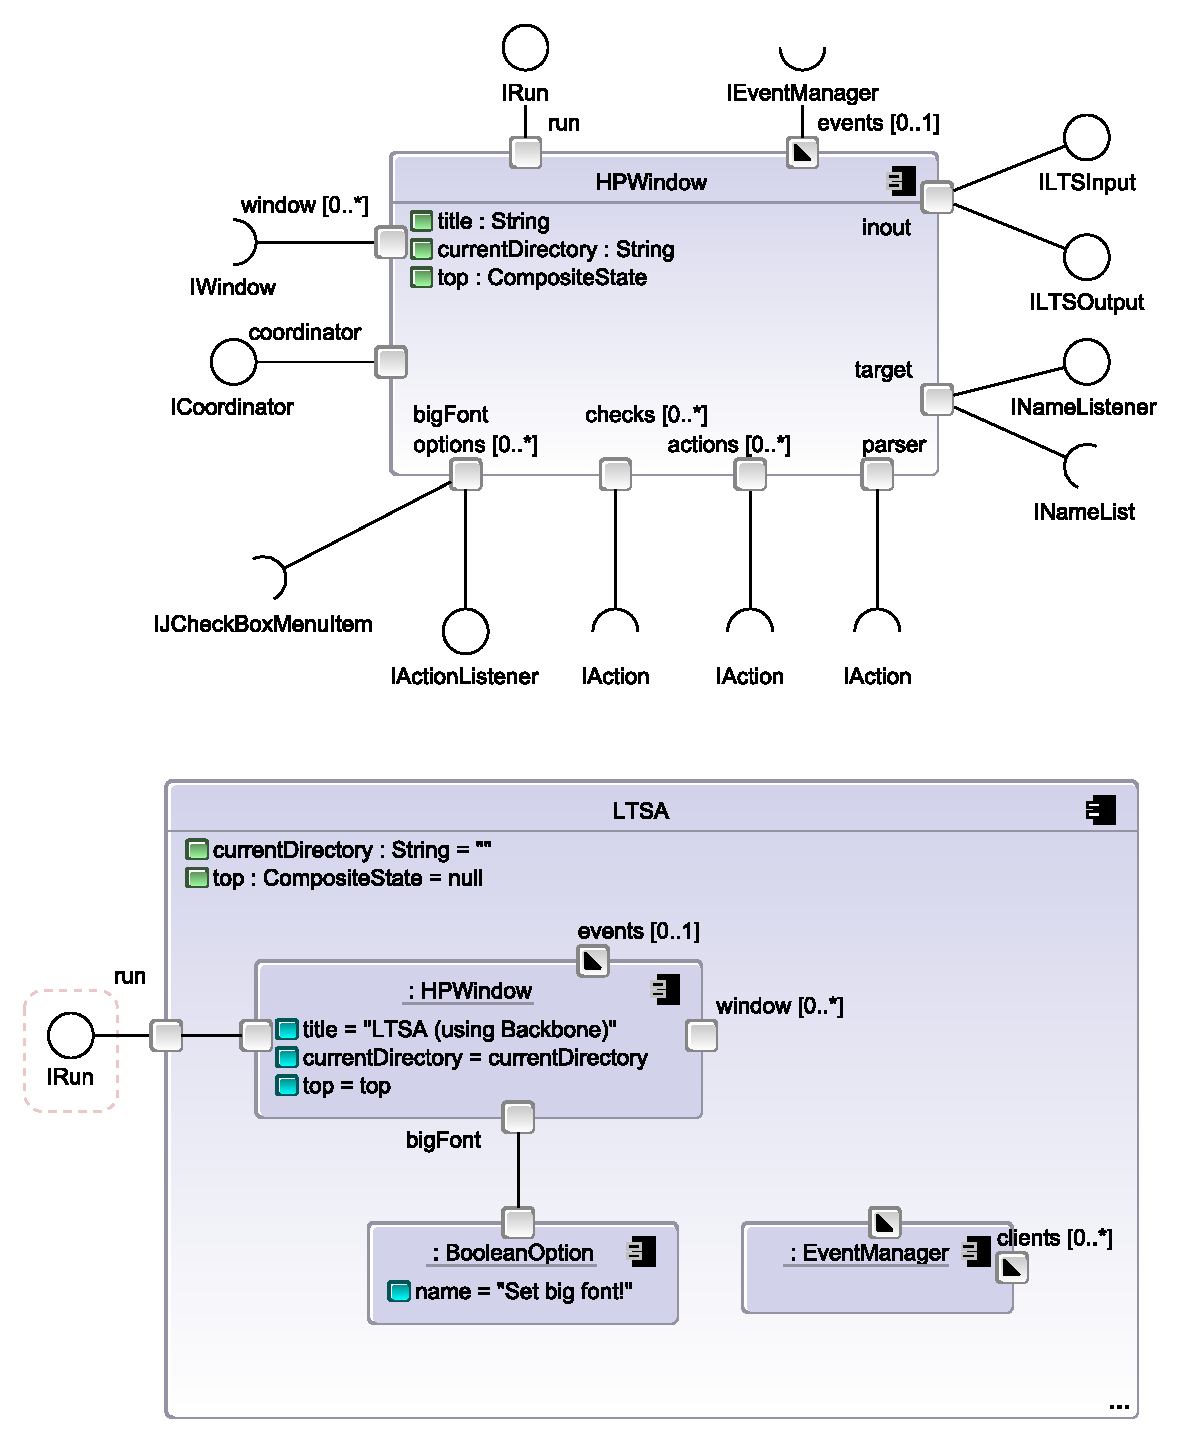
\includegraphics[width=0.8\columnwidth]{images/top-level}
\par\end{centering}

\protect\caption{\label{fig:Top-level-LTSA}Top level LTSA components}


\end{figure}


A somewhat expected, but key finding was that the best candidate classes
for turning into components were those which already implemented interfaces
(provides) and were decoupled from other classes via interfaces also
(requires). This ``interface-centric'' programming technique has
become prominent in object-oriented languages \cite{Fowler2004}{]}.
Turning LTSA classes into Evolve components simply involved adopting
this modern style more forcefully.


\subsection{Architectural Views}

As the architectectural exploration continued we realized that compositional
hierarchy was not enough to control the complexity of the diagrams
produced. Separate architectural views of the same component shown
from different ``angles'' was required and we added this feature
to Evolve.

For instance, figure \ref{fig:Top-level-LTSA} clearly does not show
all of the components at the first level of decomposition. It instead
shows only the parts which are relevant to window control. The dots
in the lower right corner of the LTSA component indicate that artifacts
have been elided.

Consider another view of the same component in figure \ref{fig:Parsing-view-of},
showing how the LTS compose action is constructed. Note that these
views are all of the same component but eliding and showing different
parts, attributes and connectors.

\begin{figure}[h]
\noindent \begin{centering}
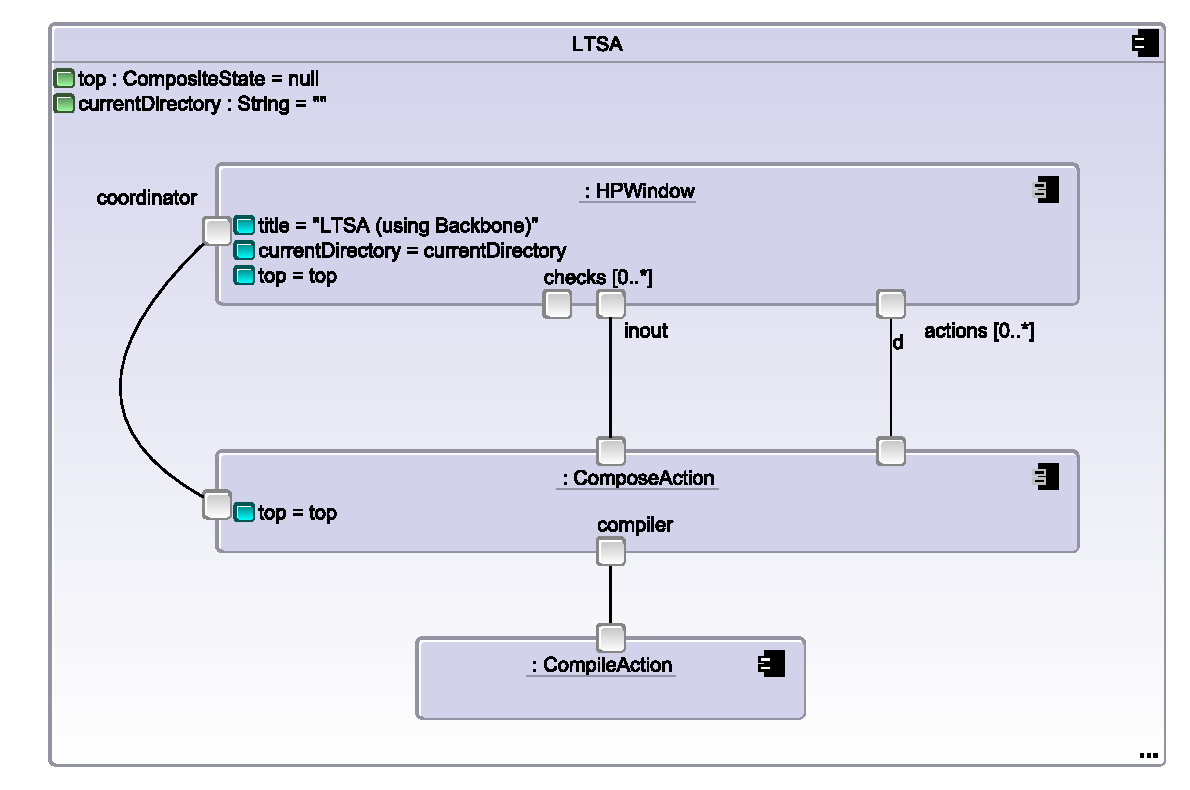
\includegraphics[width=0.8\columnwidth]{images/ltsa-compose-ltsa}
\par\end{centering}

\protect\caption{\label{fig:Parsing-view-of}Compose action view of LTSA}


\end{figure}


In our architecture description we used twelve views of the LTSA component,
reflecting the different possible graphical windows, actions and checks.


\subsection{Modeling the Evolutions}


\subsubsection*{The Ames\protect\footnote{The Ames variant originated from the NASA Ames Research Centre}
Variant}

This evolution adds extra safety checks to the base system: the first
checks for safety whilst producting multiple counterexamples, and
the second checks for safety but ignores deadlock. This system was
produced by researchers copying and modifying the source code of the
original LTSA aplication, leading to disparate codebases.

To express this application as a direct evolution we first compared
the two codebases using textual comparison tools, eventually reducing
the core difference in logic down to changes in the Analyser class
and several others.

The changes to the Analyser represented a modest proportion of the
class' overall implementation. To effect the evolved components on
top of the original architecture using our concepts we had to replace
the entire Analyser with the Ames variant reflecting the current level
of decomposition. An alternative would have been to continue decomposing
the class into finer-grained components until it reached the granularity
required to allow the changes at the correct level of abstraction.

This represents another key insight: a hierarchically decomposed system
with fine granularity allows component replacement (and hence evolution)
at the appropriate abstraction level. Architectural explication and
evolution are aligned as further decomposition for understanding and
explication presents greater opportunities to align any evolution
with the size of the changes required.

We actually chose to take a different approach - instead of direct
replacement, we instead used a component variant of the decorator
pattern \cite{Gamma1995} to add the extra checks. We evolved the
component and wrapped the former version (renamed to ExtendedAnalyser)
as per figure \ref{fig:The-wrapped-Analyser}. This is an alternative
to coarse-level replacement, allowing features to be added and existing
features masked or intercepted.

\begin{figure}[h]
\noindent \begin{centering}
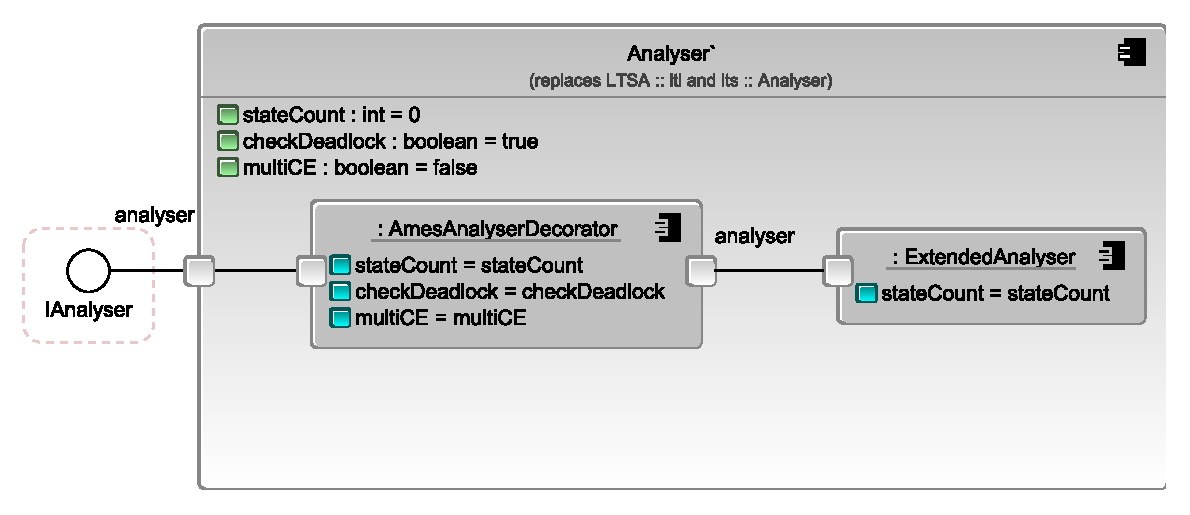
\includegraphics[width=1\columnwidth]{images/ltsa-ames-analyser}
\par\end{centering}

\protect\caption{\label{fig:The-wrapped-Analyser}The wrapped Analyser component}


\end{figure}



\subsubsection*{The DualWindow Variant}

The intention of this variant was to allow both the alphabet window
and the transitions window to be present on the screen simultaneously,
thereby improving the usability of the tool. To do this we created
the DualWindow stratum with the DualWindowcomposite which provided
the same interface IWindow as the original screen but combined the
two. We further created a factory component to allow this to be instantiated
in figure \ref{fig:The-DualWindow-component}.

\begin{figure}[h]
\noindent \begin{centering}
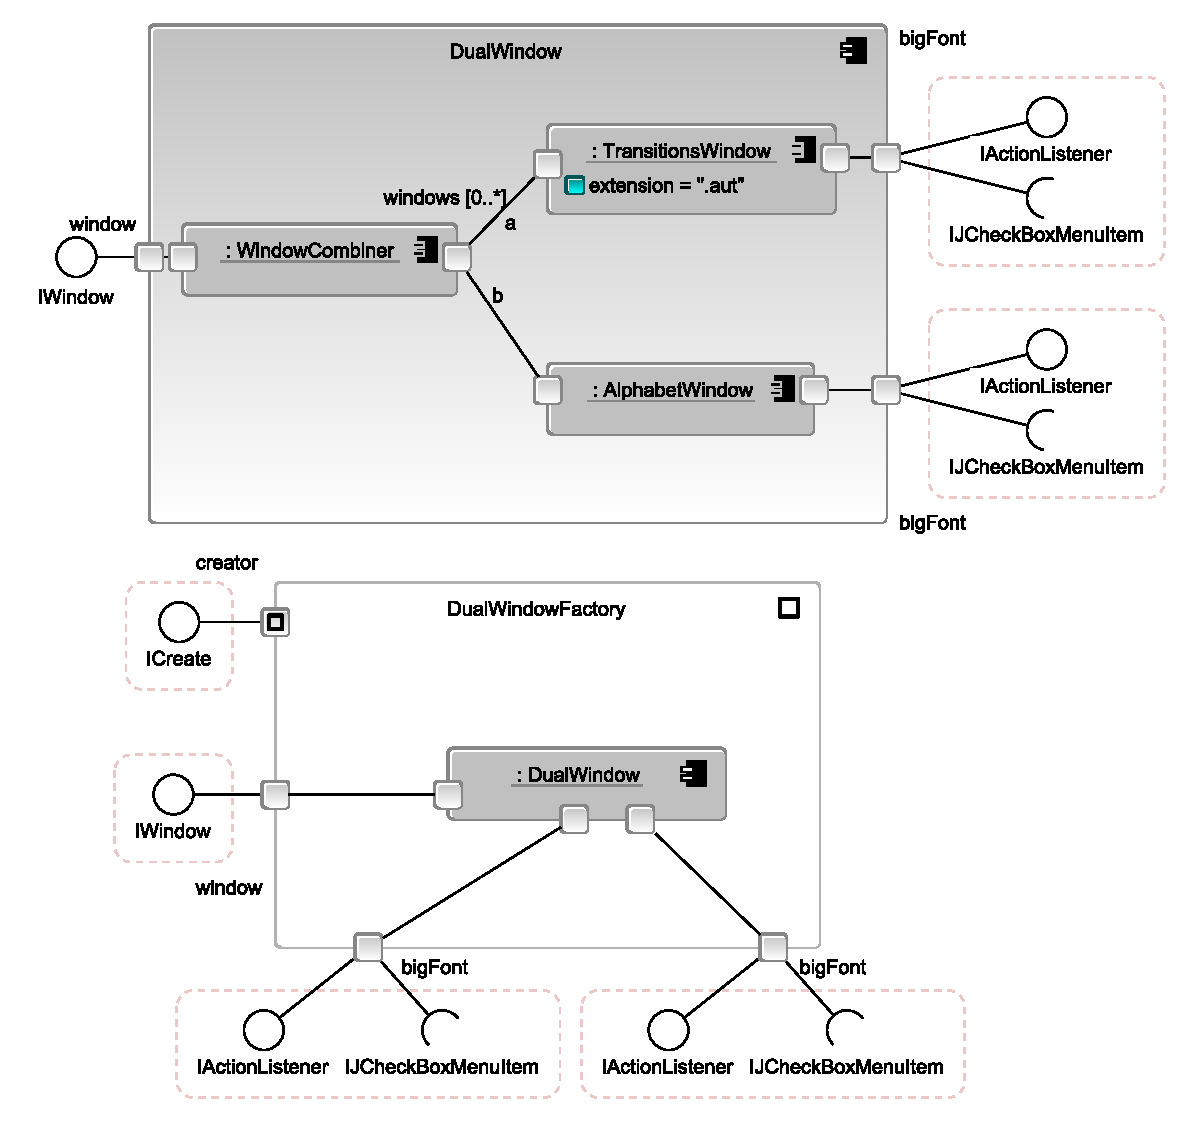
\includegraphics[width=1\columnwidth]{images/ltsa-dual-window}
\par\end{centering}

\protect\caption{\label{fig:The-DualWindow-component}The DualWindow component and
factory}


\end{figure}


Inside the DualWindow stratum, we then evolved the LTSA top-level
component and replaced the AlphabetWindowFactory part with a DualWindowFactory
one. We also replaced the HPWindow part with an instance of the same
type but with amended properties. This is shown in figure \ref{fig:Evolving-LTSA-to}.
The Backbone text underneath describes the deltas.

\begin{figure}[h]
\noindent \begin{centering}
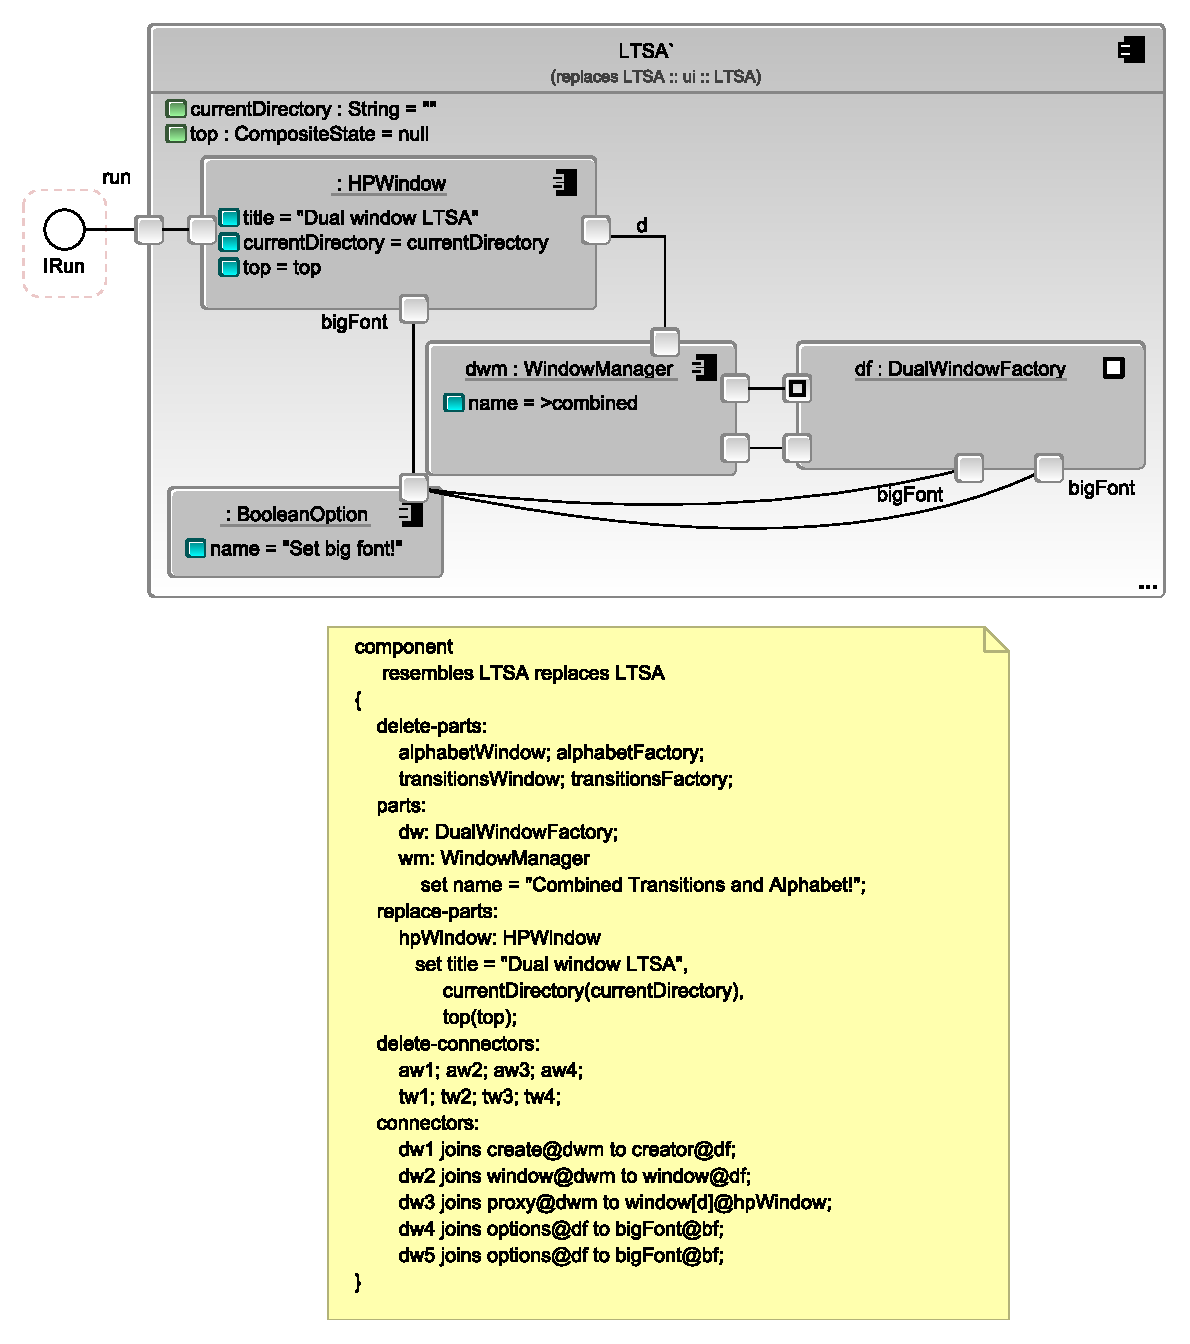
\includegraphics[width=1\columnwidth]{images/ltsa-dualwindow-evolution}
\par\end{centering}

\protect\caption{\label{fig:Evolving-LTSA-to}Evolving LTSA to support dual windows}


\end{figure}



\subsection{Merging the Evolutions}

To merge the evolved architectures we created another (empty) stratum
called combined which depends on the two variant strata (figure \ref{fig:Combining-the-evolutions}). 

\begin{figure}[h]
\noindent \begin{centering}
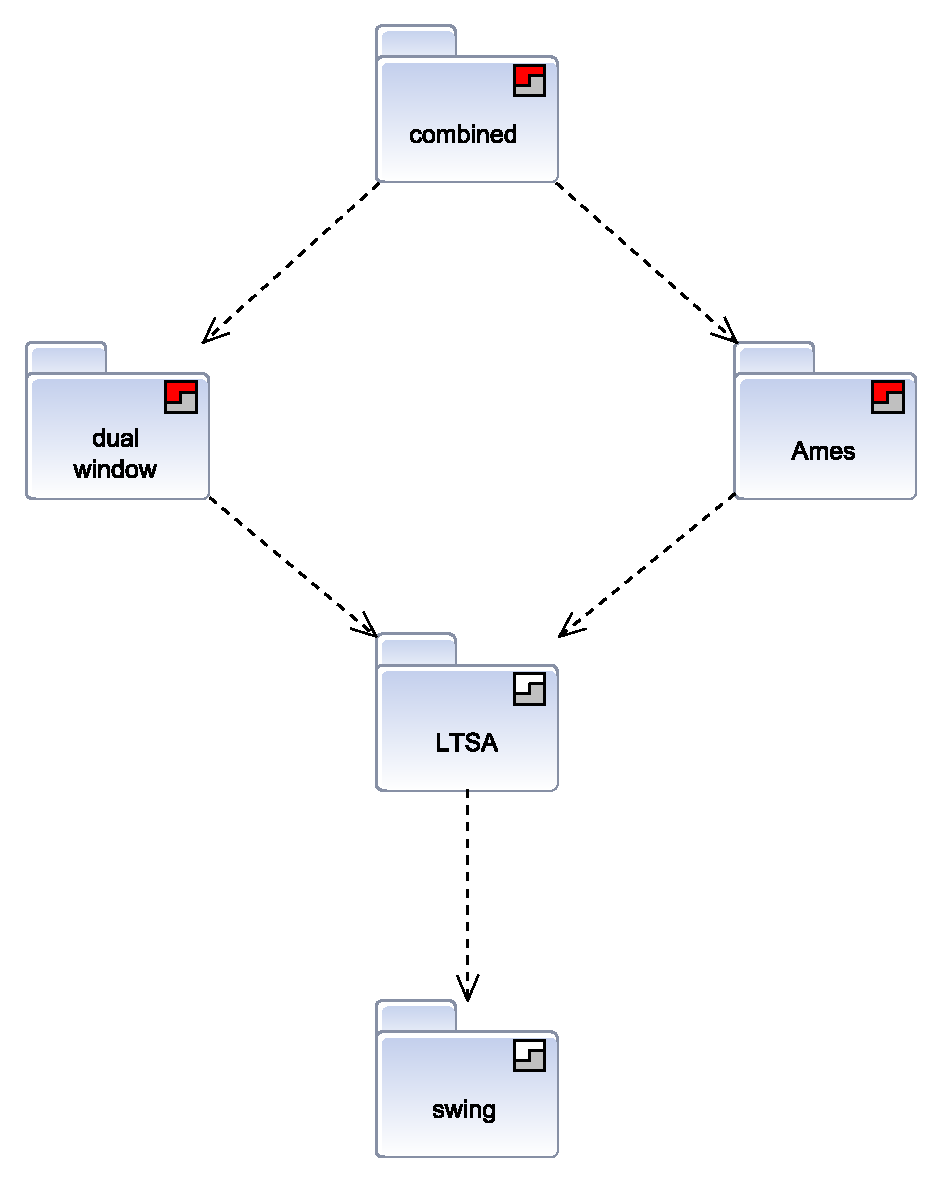
\includegraphics[width=0.6\columnwidth]{images/ltsa-stratum-extensions}
\par\end{centering}

\protect\caption{\label{fig:Combining-the-evolutions}Combining the evolutions using
a further stratum}


\end{figure}


\begin{figure}[h]
\noindent \begin{centering}
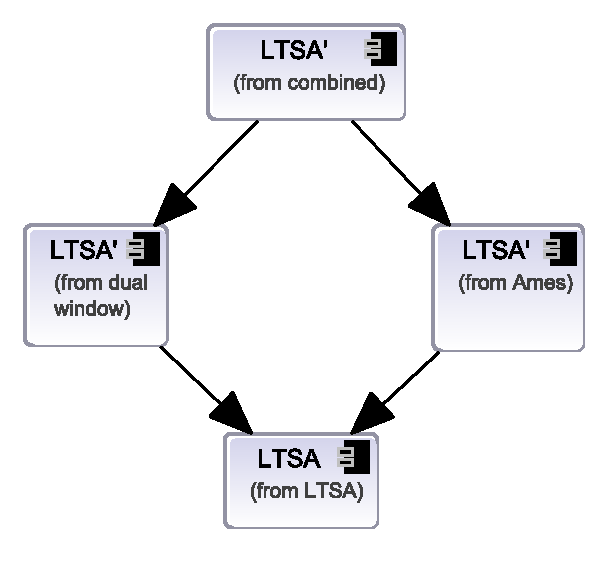
\includegraphics[width=0.45\columnwidth]{images/expanded}
\par\end{centering}

\protect\caption{\label{fig:The-expanded-LTSA}The expanded LTSA resemblance graph}
\end{figure}


\begin{figure}[th]
\noindent \begin{centering}
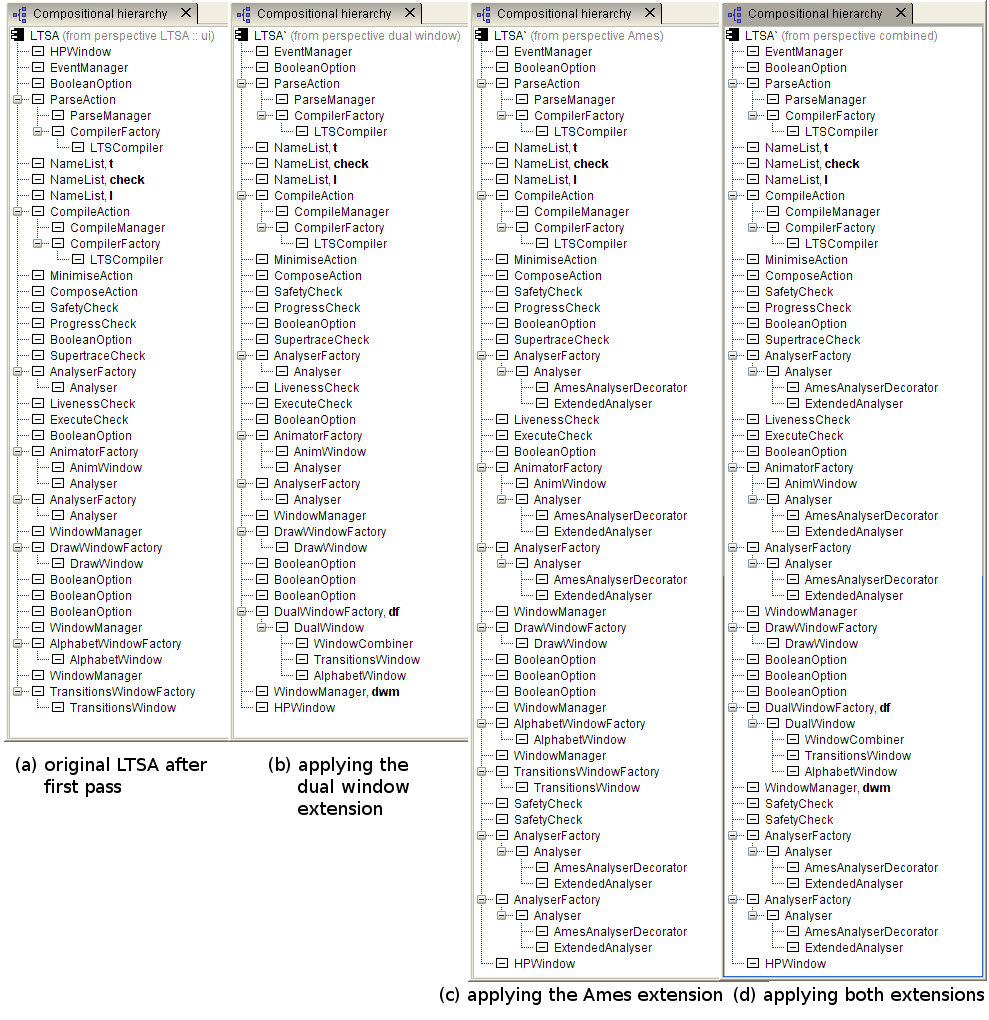
\includegraphics[width=0.5\paperwidth]{drawings/ltsa-compositions}
\par\end{centering}

\protect\caption{\label{fig:Compositional-history-of}Compositional history of the
LTSA evolutions and merge}
\end{figure}


According to the rules described earlier this strata arrangement leads
to a rewriting of the resemblance relations to incorporate the independent
evolutions in a unified graph. The expanded resemblance graph of the
LTSA component from the perspective of the combined stratum is shown
in figure \ref{fig:The-expanded-LTSA}. We can see that the independent
evolutions result in independent branches of the graph and that the
combining stratum joins them back again. This happens automatically
- if a combining stratum does not declare an evolution then the net
effect of the rules is as if a default implicit evolution is created
to ensure a merge.

In this case a full error check revealed there were no conflicts requiring
resolution, and the two variants were able to be combined and run
together successfully. If conflicts had actually occurred these could
have been rectified by explicitly evolving the LTSA component in the
combined stratum and adjusting or replacing the erroneous constituents
using deltas.

Figure \ref{fig:Compositional-history-of} shows the compositional
history of the LTSA evolutions. The depth and breadth of composition
changed over time reflecting the deepening explication of the architecture
and the evolution of the components in each of the variants.


\subsection{Conclusion}

Incorporating the Evolve approach into a mature application involves
initially decomposing the architecture down to a sufficient level
of granularity to enable the evolutionary variants to be expressed
via component replacements. This relies on refactoring the architecture
to turn identified candidate classes into components with both provided
and required interfaces. This accords well with best practice object-oriented
design which uses interfaces heavily for decoupling.

Decomposing the architecture into finer-grained components and allowing
evolution to be clearly expressed align neatly - these cooperating
forces lead to a system with an explicit architecture which can be
evolved with commensurate effort related to the size of the change
required.

Branching and merging of evolutionary variants can be explicitly represented
using strata. The branches and joins of the resultant expanded resemblance
graphs reflect the strata dependencies. Further, the same constructs
allowing evolution allow any merge conflicts to be rectified regardless
of the level of the conflict in the compositional hierarchy.


\section{Wider Applicability of the Intrinsic Approach}

The intrinsic approach is applicable to any system that is expressed
naturally via a compositional hierarchy, where evolutionary forces
over time lead to a decomposition at a fine-grained level so that
replacement can operate at the desired level of abstraction. In applying
our approach, we found a number of candidates that satisfied these
requirements: nested statecharts, user interface construction, component-based
framework development and extensible, plugin-based systems.


\subsection{Nested Statecharts}

State machines are a powerful way to explicitly represent the states
and possible transitions that a system may go through \cite{Mencl2004}.
The full set of transitions are fully explicated, giving an exhaustive,
testable overview of the behavior of the system.

Statecharts are a visual representation of a state machine, where
states are shown typically as rectangles and transitions as lines
between them \cite{Harel1987}. Harel further demonstrated that nested
state charts provide the ability to classify complex system behavior
into a hierarchy, allowing the system to be reasoned about at different
levels of abstraction.

To explore our approach applied to this domain, we modeled a fader
for an audio control desk on a commercial radio broadcast system the
authors previously worked on. A fader has audio control of a single
device such as a CD player, and can start, pause and stop it and control
where the output is heard.


\subsubsection{Modeling Statecharts Using Design Patterns}

State machines in object-oriented systems are usually represented
using a variant of the state pattern \cite{Gamma1995}. For instance,
a fader would be modeled as per the class diagram in figure \ref{fig:Modeling-states-using}.

\begin{figure}[h]
\noindent \begin{centering}
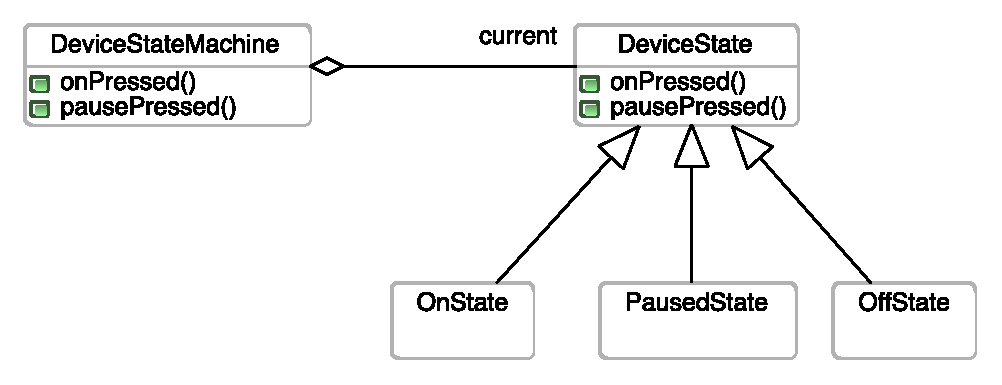
\includegraphics[width=0.7\columnwidth]{phd-images/oo-state-advanced}
\par\end{centering}

\protect\caption{\label{fig:Modeling-states-using}Modeling states using design patterns}


\end{figure}


Note that transitions are not explicit and are instead represented
as programming logic within each state. Via the pattern guidelines,
this means that every state contains a hardcoded reference to the
state classes which it transitions to, reducing our ability to add,
delete or modify states and transitions without having to replace
a large number of them. For instance, the transition between the OFF
and ON state is encoded in the \texttt{OffState} class as:
\begin{lyxcode}
{\footnotesize{}if~(onTransition)~\{}{\footnotesize \par}

{\footnotesize{}~~context.setState(new~OnState());}{\footnotesize \par}

{\footnotesize{}~~...}{\footnotesize \par}
\end{lyxcode}
In audio it is typical to move from the OFF state, to a CUE state
where the audio is played directly only to the presenter, then to
the ON state where the audio is broadcast. However, to do this we
would have to add \texttt{CueState} and also replace \texttt{OffState}
which hardcodes the existing transition. Furthermore, the set of possible
events are hardcoded inside the \texttt{DeviceStateMachine}, meaning
we would have to also modify this to add a cure event.

This hardcoding of transitions inside each state limits the extensibility
of the state machine when coded in this paradigm. 


\subsubsection{Modeling Statecharts Using the Intrinsic Approach}

To apply the intrinsic approach, we initially noted the similarity
between nested component structure and nested statecharts, and between
connectors and transitions. By adopting a pattern regarding entry
and exit actions, and transition handoff from one state to another,
we could translate states into components and and transitions into
connector between ports. This allowed us to apply the intrinsic approach
to statechart evolution.

Figure \ref{fig:Modeling-a-state} shows the results of modeling the
states via components, giving rise to a dispatcher component that
mediated the ownership of the current state between the three concrete
states. The transitions were modeled as connectors between states,
and ports acted as guards.

\begin{figure}[h]
\noindent \begin{centering}
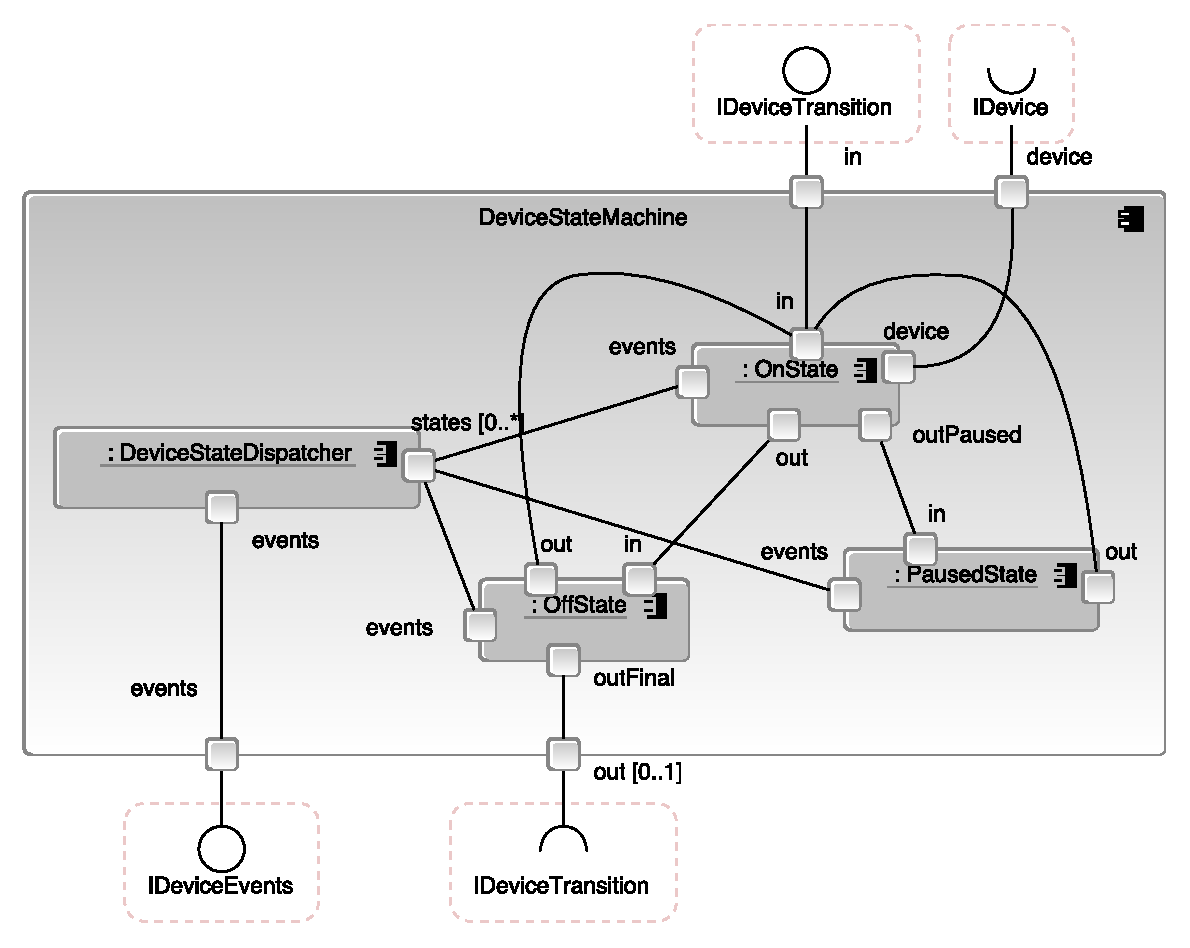
\includegraphics[width=1\columnwidth]{phd-images/component-fullstate-advanced}
\par\end{centering}

\protect\caption{\label{fig:Modeling-a-state}Modeling a state machine via components}


\end{figure}


The \texttt{DeviceStateDispatcher} component was generic, reusable
code and could be inserted via rule, allowing us to omit it from the
visual presentation. We further finessed the appearance so that it
more closely resembled that of a traditional statechart, as shown
in figure \ref{fig:Adjusting-the-appearance}.

\begin{figure}[h]
\noindent \begin{centering}
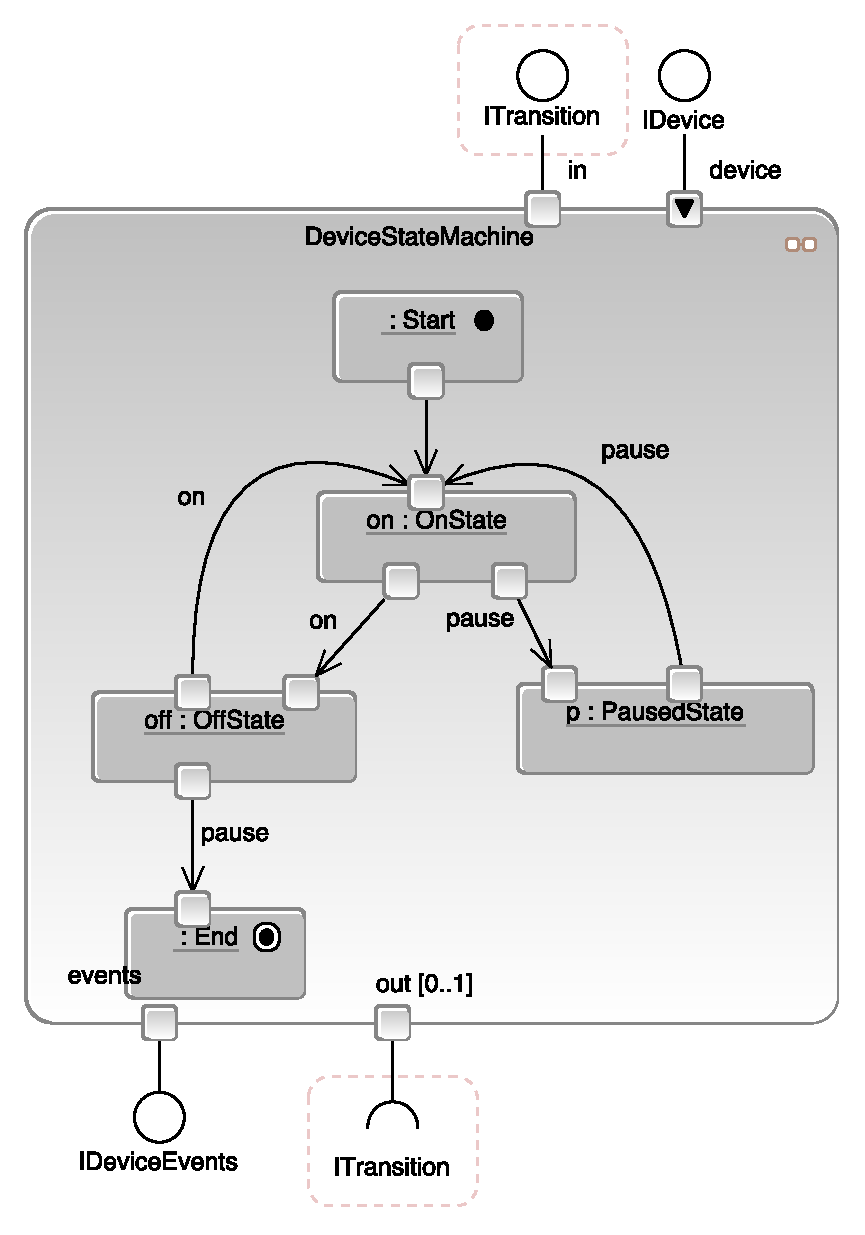
\includegraphics[width=0.65\columnwidth]{phd-images/stereo-fullstate-advanced}
\par\end{centering}

\protect\caption{\label{fig:Adjusting-the-appearance}Adjusting the appearance}
\end{figure}


We then evolved the statechart component to add a CUE state, allowing
audio to be previewed on an off-air audio bus. This used resemblance
and replacement to add the additional state component and adjust several
connectors, but required no further changes or replacements. Figure
\ref{fig:Evolving-to-add} shows the final chart.

\begin{figure}[h]
\noindent \begin{centering}
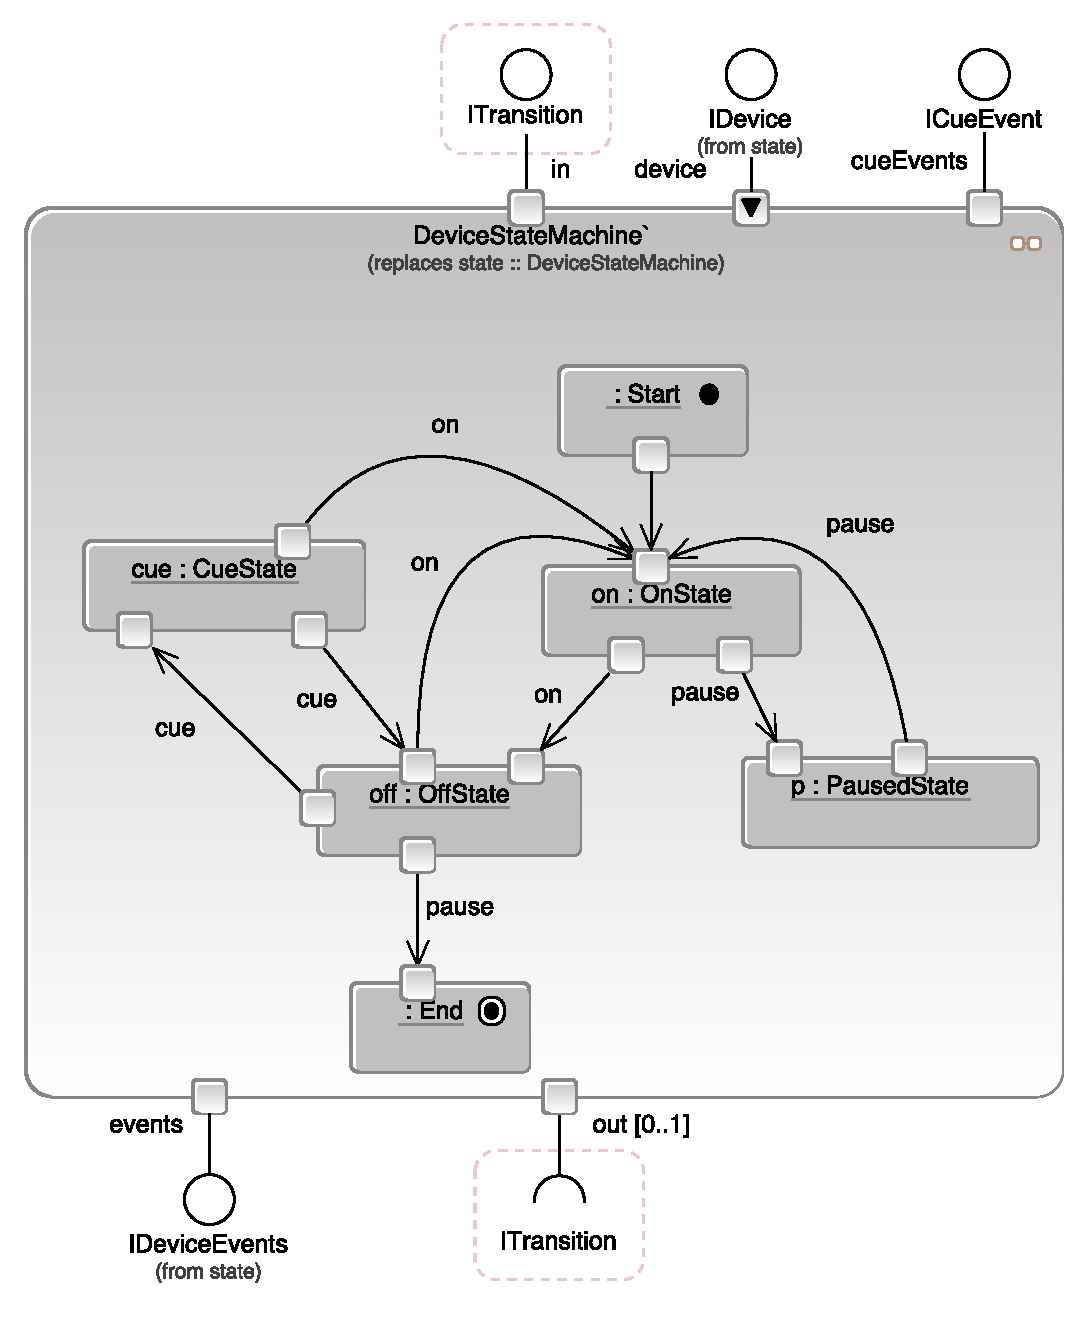
\includegraphics[width=0.8\columnwidth]{phd-images/added-cue-state-advanced}
\par\end{centering}

\protect\caption{\label{fig:Evolving-to-add}Evolving to add the CUE state}


\end{figure}


By making the transitions explicit and not hardcoded into the states
themselves, the system is more understandable and more extensible.


\subsection{User Interface Construction}

User interfaces are often constructed in a component-oriented way,
where connections between user interface components (aka ``widgets'')
are created using builders and visual tools. The JavaBeans specification
was created with these builders and visual construction in mind -
through the use of lexical conventions for ``getters'' and ``setters''
and reflection, instances of these widgets can be manipulated visually
\cite{O'Neill1998,Network2006}.

To support this paradigm, we implemented an importing facility into
our Evolve case tool, to allow beans to be represented as Backbone
components (c.f. \ref{sub:Compatibility-with-Existing}). We imported
the Swing library \cite{Hoy2002} in its entirety. In this model,
connectors represent the getting and setting of bean references from
Swing components.

As shown in figure \ref{fig:Evolving-LTSA-to}, we were able to successfully
model and evolve a complex Swing-based UI system.

For another project, we needed to model the Google Web Toolkit system
(GWT) \cite{GWT,GWT-Apps} for constructing Web applications. This
also uses a variant of the JavaBeans model, but translates the Java
code into Javascript in order to run the application in a browser.

Figure \ref{fig:A-graphical-widget} shows a widget for adding a car
in a car rental application. This widget was part of a larger application
which was evolved to add various features using the intrinsic approach,
without particular restrictions due to the more limited runtime environment
or unusual translation requirements.

\begin{figure}[h]
\noindent \begin{centering}
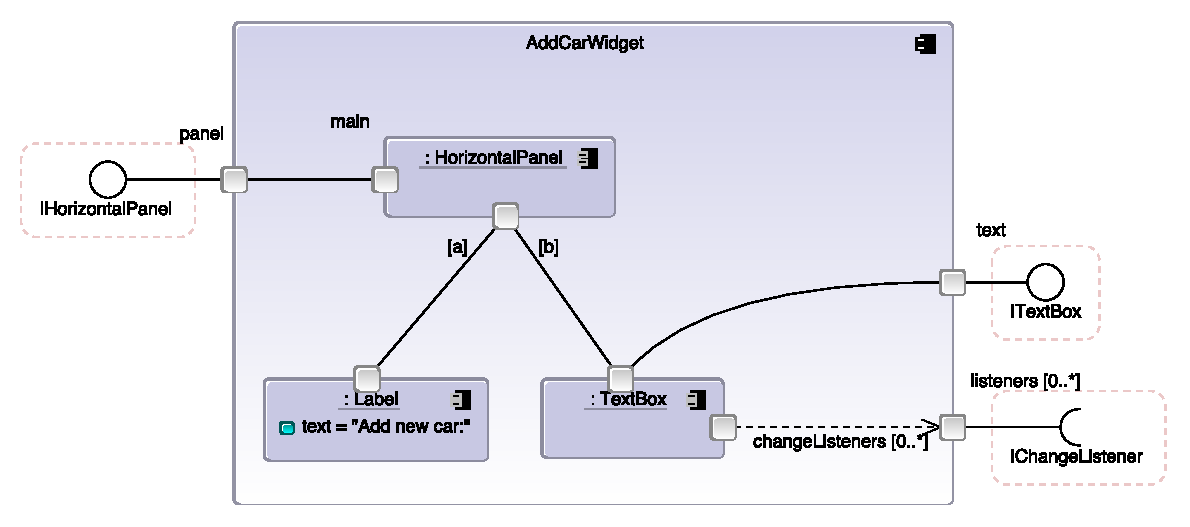
\includegraphics[width=1\columnwidth]{phd-images/add-car}
\par\end{centering}

\protect\caption{\label{fig:A-graphical-widget}A graphical widget from a GWT application}


\end{figure}


The runtime environment for GWT is Javascript and there are limited
reflection capabilities available to a translated Java application.
As such, reflection could not be used to instantiate the system. To
deal with this, we wrote a short addition to the Evolve toolset which
generated a Java program for the flattened representation of the compositional
hierarchy, which directly made the calls required to instantiate the
system.

For instance, part of this generated code looked as follows:
\begin{lyxcode}
{\footnotesize{}HorizontalPanel~h1~=~new~HorizontalPanel();}{\footnotesize \par}

{\footnotesize{}Label~l1~=~new~Label();}{\footnotesize \par}

{\footnotesize{}l1.setText(``Add~new~car:'');}{\footnotesize \par}

{\footnotesize{}h1.add(l1);}{\footnotesize \par}

{\footnotesize{}...}{\footnotesize \par}
\end{lyxcode}
Using this approach, Backbone can run in environments with extremely
constrained capabilities.


\subsection{Component-based Framework Development}

Frameworks are reusable software systems which are designed to be
reused and extended by other parties \cite{Froehlich1997,Fayad1997}.
The primary characteristic of a framework is a property known as the
Hollywood Principle, or Inversion of Control \cite{Gamma1995}. This
is known colloquially via the expression ``don't call us, we'll call
you''. In other words, the framework owns the control of the program,
and delegates down to the extensions where required.

This approach to development requires that a framework contain a set
of pre-planned extension points. It is extremely common when building
a system around a framework to find that the system requirements cannot
be met using the existing extension points, and it is necessary then
to evolve the framework to add new points. This need to feed back
to a central architecture typically leads to great delay \cite{Bosch2000}
and also pollutes the framework with extension points that may only
satisfy a small number of systems.

The intrinsic approach resolves these problems by placing the ability
to adjust and extend the framework (and hence extension points) in
the hands of the users of the framework (extension developers), not
just in the hands of the original creators. The intrinsic approach
holds alterations as deltas, allowing these changes to be fed back
to the creators for future inclusion if needed, without holding up
the extension developers. Further, the alterations do not need to
be fed back to the creators if they are not sufficiently general,
and can simply be maintain by extension developers. In this way, the
core framework does not get polluted with every required extension
point.

Another problem faced by users of a framework is that they might make
changes locally to the framework, but then need to reapply those changes
when the creators publish a new version. In the intrinsic approach,
any changes made by an extension developer would be held as deltas,
allowing them to simply repoint their strata dependencies at the new
framework version and have the changes automatically applied.


\subsection{Plugin Systems}

Many extensible systems allow third party programmers to create and
install plugins which enhance and adapt the application's functionality
for new requirements. Such an application is typically designed as
a black box with extension points and a loading scheme for plugins,
which then register themselves with the system \cite{Chatley2003,Chatley2004}.

This has an obvious corollary with frameworks, in that no system can
fully predict the full set of extension points required. As such,
a developer writing an extension will often need to request extra
extension points from the base application developers, which leads
to serious sequencing issues and time delays \cite{Bosch2000}.

Some plugin systems are structured fully out of plugins to resolve
this dilemma. For instance, the Eclipse integrated development environment
is composed completely of semantically versioned plugins, allowing
any plugin to be replaced \cite{Consortium2006,Delap2006}. 

However, even this more complete model has a problem - plugins are
both the unit of deployment and the unit of replacement. Combined
with the fact that plugins are non-hierarchical, this creates a number
of problems, which we will now elaborate on.

For instance, consider that to make their plugin E, a plugin developer
requires an additional extension point in a large, core plugin C which
is owned by the creators of the application. The change is relatively
small, but results in a new version of C, say v1.0.1, which must then
be released to anyone who wants to use plugin E. However, because
C is not owned by the plugin developer, it will be necessarily overwritten
by any updates from the base developers. In other words, because the
only unit of change is a plugin, which is also the unit of ownership,
even a small change can result in a large amount of work and an infeasible
developer workflow and deployment situation. This situation is made
greatly worse by the fact that for ease of management, a plugin is
typically coarse-grained and encompasses a large amount of functionality.

The intrinsic approach addresses these problems by having separate
entities for each concept. A stratum is the unit of ownership, a component
or interface is the element of change, and replacement and resemblance
allow a stratum owned by an extension developer to own changes to
a component from a stratum owned by the base developers.

To map the above plugin dilemma onto the intrinsic approach, consider
that the extension developer would have a stratum SE, which contained
their plugin E represented as one or more components. The base developer
would have a stratum SC which contained their plugin C represented
as components also. In this case, C is a composite which is made up
of other parts including an instance of CSub.

To make the change to add the required extension point, the stratum
SE would then contain an evolution of the components in SC to introduce
the required extension points, at the appropriate level in the compositional
hierarchy. The SC stratum does not have to change, allowing new versions
of C to be used without affecting E. This is shown in figure \ref{fig:Addressing-the-plugin}.

\begin{figure}[h]
\noindent \begin{centering}
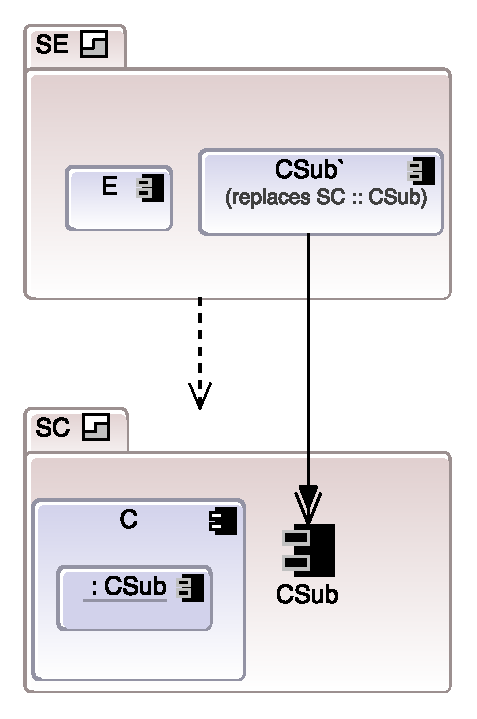
\includegraphics[width=0.3\columnwidth]{images/plugins}
\par\end{centering}

\protect\caption{\label{fig:Addressing-the-plugin}Addressing the plugin dilemma}


\end{figure}



\section{Developer Workflow in a Distributed Environment}

Our approach is designed to support developers extending and evolving
a system in a setting where (in the worst case) the parties may have
limited communication and may not share networks or other resources.
For instance, the initial system can be created by one party, who
can then export the definition and implementation to other parties
who can evolve it and branch it without affecting the original definitions.
We can later merge these branches back into a single model and rectify
any structural conflicts using the same constructs available for evolution.

Consider how development and evolution of the LTSA system (section
\ref{sec:Applicability-to-Mature}) might have proceeded. Firstly,
the original architecture and implementation of the system would have
been created by developer X. At this point, X has only the LTSA stratum
present in their system, as shown in figure \ref{fig:LTSA-System-as}.

\begin{figure}[h]
\noindent \begin{centering}
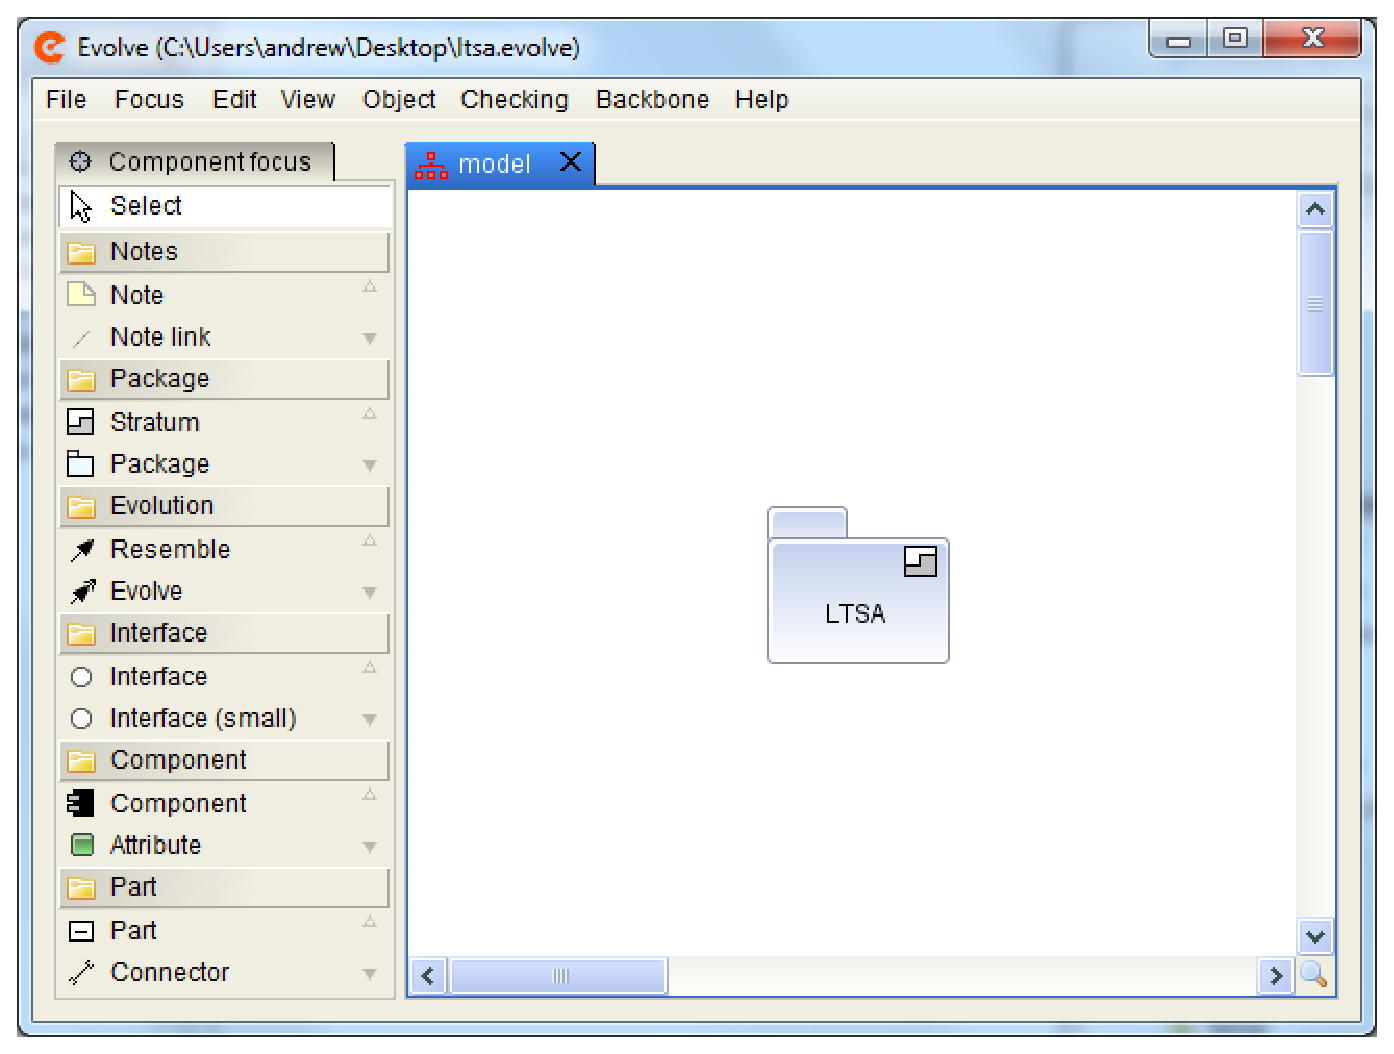
\includegraphics[width=0.8\columnwidth]{drawings/wf-original}
\par\end{centering}

\protect\caption{\label{fig:LTSA-System-as}LTSA System as seen by its creator}


\end{figure}


Developers Y and Z now wish to separately evolve the system. To facilitate
this, X exports the LTSA stratum from their environment and distributes
both the exported stratum (.evolve file) and compiled files representing
the implementation (jars) to both developers.

Y and Z each create their own extension strata in their separate environments.

Consider that Y has decided to implement the dual window extension.
Y will import the LTSA stratum (as read-only because they do not own
this) and create the dual window stratum as shown in figure \ref{fig:The-system-as-1}.

\begin{figure}[h]
\noindent \begin{centering}
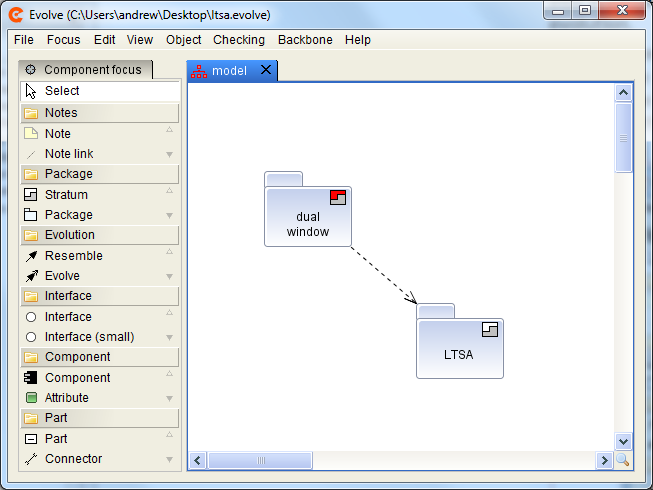
\includegraphics[width=0.8\columnwidth]{drawings/wf-dual}
\par\end{centering}

\protect\caption{\label{fig:The-system-as}The system as seen by Y}


\end{figure}


Z has decided to implement the Ames evolution. Z imports the LTSA
stratum (again as read-only) and creates the Ames stratum as shown
in figure \ref{fig:The-system-as-1}.

\begin{figure}[h]
\noindent \begin{centering}
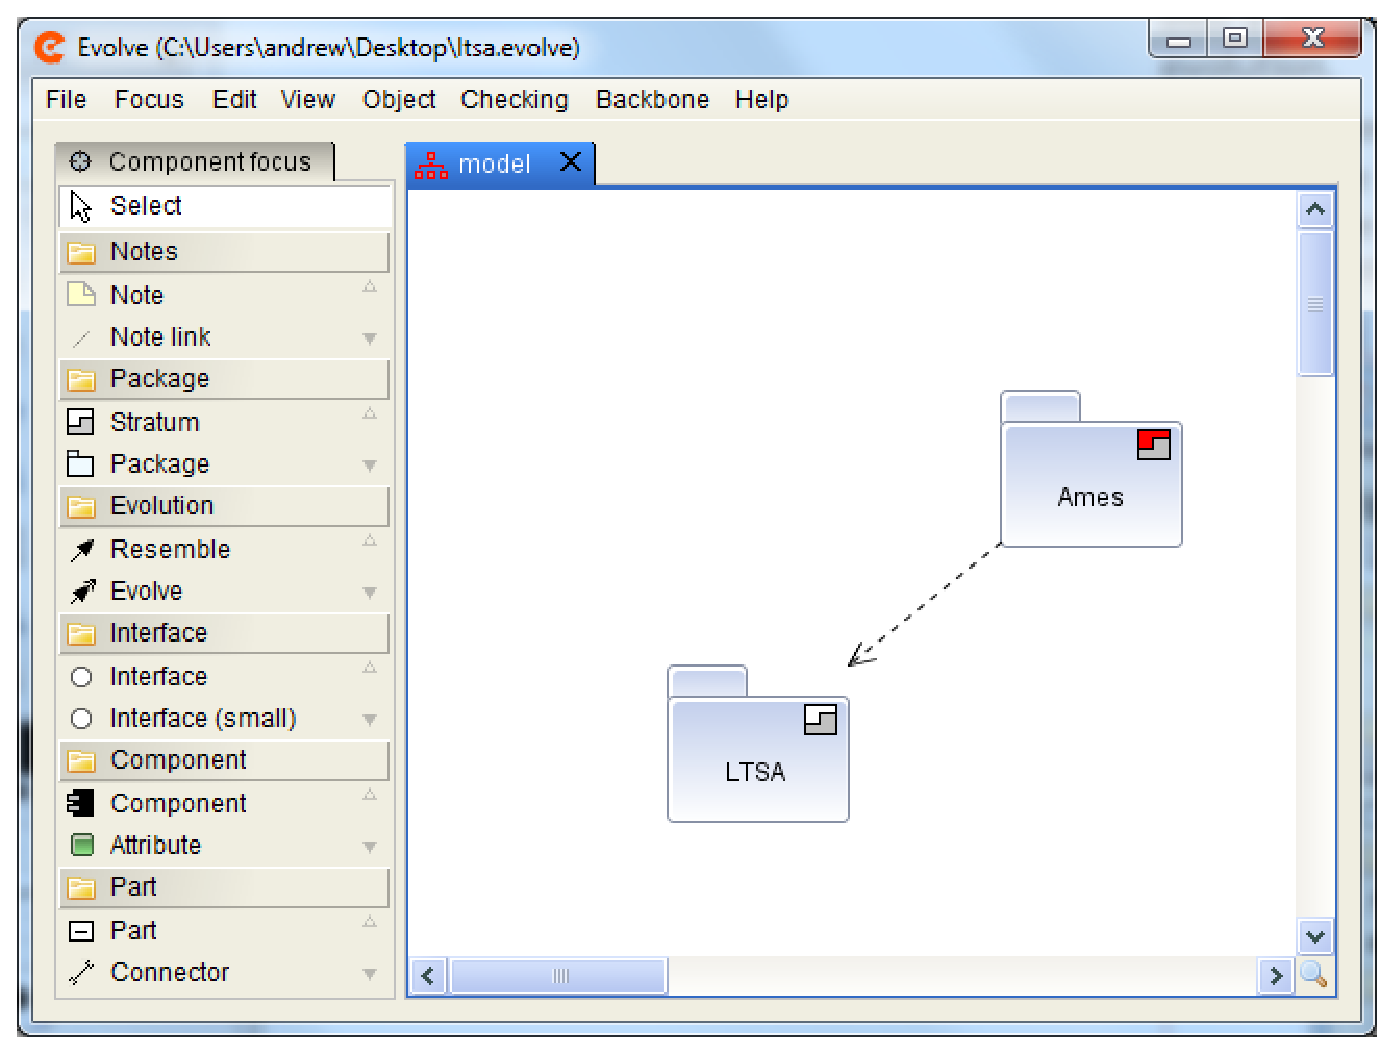
\includegraphics[width=0.8\columnwidth]{drawings/wf-ames}
\par\end{centering}

\protect\caption{\label{fig:The-system-as-1}The system as seen by Z}


\end{figure}


Note that Y and Z are free to make any changes to the base architecture
as long as the evolutions are contained in the stratum that they own.
They cannot directly edit the LTSA stratum as this is owned by X.

Now consider that X wishes to accept both extensions from Y and Z
and merge them into a common architecture. To do this, X imports both
the dual window and Ames strata (and associated implementation jars)
into their original environment. The two imported strata are marked
as read-only, as X does not own these. To create the merge, X further
creates the combined stratum. Any structural conflicts can be rectified
in that stratum which X owns. This is shown in figure \ref{fig:Merging-the-two}.

\begin{figure}[h]
\noindent \begin{centering}
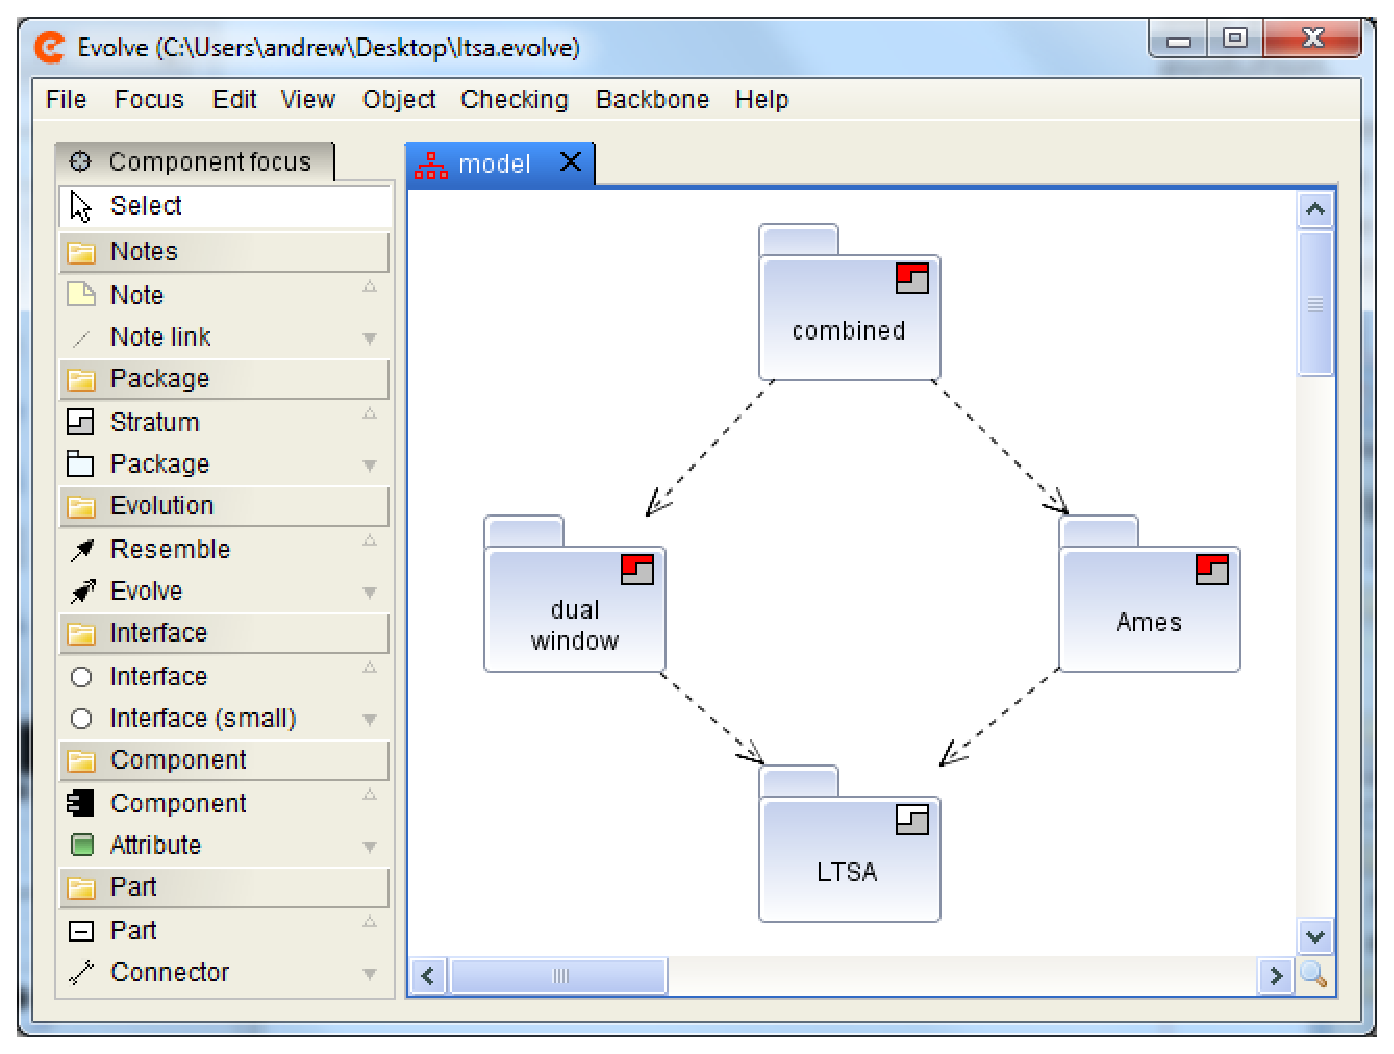
\includegraphics[width=0.8\columnwidth]{drawings/wf-merged}
\par\end{centering}

\protect\caption{\label{fig:Merging-the-two}Merging the two evolutions}


\end{figure}


The general principle in a distributed setting is that the import
and export of strata allow for sharing and collaboration. We export
strata that we own, and import strata that are owned by others. We
only directly edit our own strata, but we can express any changes
to architectures created by imported strata by creating our own further
stratum that depends on the imported ones.

The sharing of artifacts in this disconnected way is made possible
by the use and allocation of UUIDs for each element. This guarantees
that accidental conflict due to human readable names being the same
will not occur.


\section{Analysis and Assessment}

In this section we distill a set of interesting properties for an
architectural approach to evolution and evaluate Evolve against these.
In the next section we use these properties to assess related work
against the same criteria.


\subsection{\label{sub:Essential-Properties-of}Properties for an Architectural
Approach to Evolution}


\subsubsection*{Unconstrained architectural alterations}

An approach should allow the architecture of a system to be altered
in (possibly) unplanned ways to accommodate new features and requirements.
The unit of change should be architectural (component, interfaces,
constituents) and there should be no arbitrary constraints on what
type of features can be added or removed. It should also be possible
to switch between the base system or the evolved system as desired
- an evolution should not affect or destructively edit the base architecture.

Evolve supports this property via deltas against components and interfaces.
Components can be evolved by adding, replacing or deleting at the
level of attribute, connector, part or implementation class mappings.
Interfaces can be evolved at the level of operation or implementation
realization. This does not affect the base architecture - the evolution
is instead recorded as a set of deltas in a stratum which depends
on the base stratum, allowing the architect to switch between the
base and evolved system.

This level of expressiveness clearly allows invalid systems to be
created. We supplement this freedom with a comprehensive set of checks
which determine the structural wellformedness of a system. No behavioral
checking is currently done - this is considered in future work.


\subsubsection*{Alterations at the correct level of abstraction}

The architecture should be able to be evolved at the appropriate abstraction
level. Further the level of change required should be commensurate
with the actual change in functionality. Sometimes coarse-grained
replacement is required when making large-scale changes, at other
times fine-grained adjustment is all that is needed.

A hierarchical component model like the one used by Evolve meets the
above property nicely. It neatly resolves the conflict between coarse
and fine-grained components by allowing larger components to be built
up from instances of smaller ones. If a hierarchical model is not
used, for instance in plugin systems, then it can be difficult to
evolve the architecture at the correct level of abstraction.


\subsubsection*{Branching the architecture}

It should be possible to create independent branches of a system,
reflecting that work may proceed in parallel even within the same
organization.

Evolve supports this property via the stratum concept which allows
a set of changes to be grouped, and dependencies to be explicitly
indicated. Two strata that have no visibility of each other via transitive
dependencies, but nevertheless share common strata in their dependency
graph, are independent branches of the same underlying system. An
example of this is shown in figure \ref{fig:Branches-and-a}.

\begin{figure}[h]
\noindent \begin{centering}
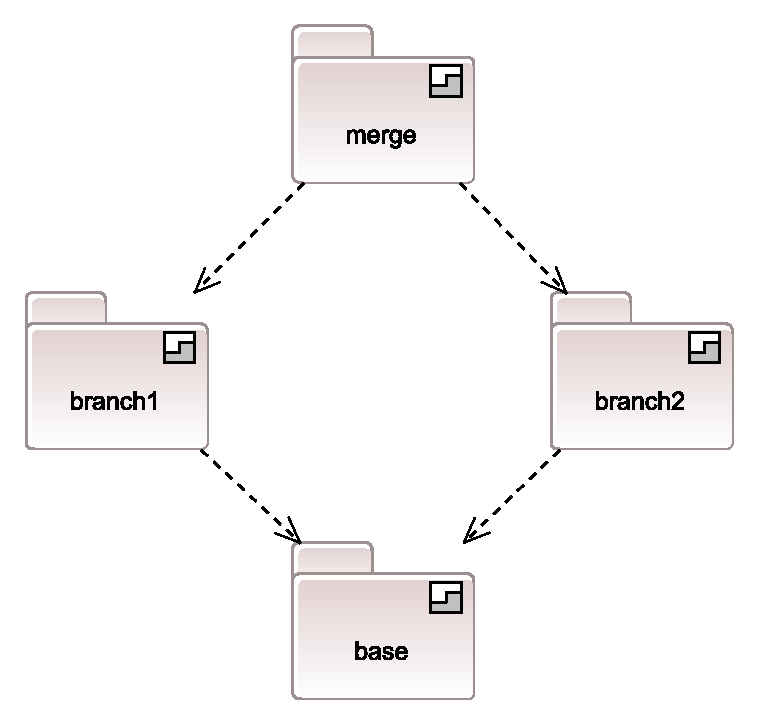
\includegraphics[width=0.6\columnwidth]{images/branching}
\par\end{centering}

\protect\caption{\label{fig:Branches-and-a}Branches and a merge of a base system}
\end{figure}



\subsubsection*{Merging and conflict resolution}

It should be possible to merge branches back into a single architecture,
where any inconsistencies or conflicts are detected and can be corrected
architecturally at the appropriate level of abstraction.

We support this via a single stratum which depends on two or more
branch strata, as shown in figure \ref{fig:Branches-and-a}. Under
the rules of section \ref{sec:A-Formal-Description}, separate evolutions
of a component in branches will result in an expanded resemblance
graph which is similarly branched. Simple conflicts are detected where
the same constituent has been deleted or replaced separately in each
branch, requiring a further evolution in the merge stratum to choose
one of the outcomes as preferred.

More complex structural conflicts are detected by checking the rules
against the merged architecture. Any violation of the rules can be
dealt with via another evolution, at the desired level in the composition
hierarchy.


\subsubsection*{Immutable, released system}

Once an extension has been formally released into a distributed setting,
the definitions within it must be regarded as immutable. Without this
property, it would be impossible to know definitively which variant
of the extensions and its definitions were correct. Typically, this
immutability is denoted by assigning a semantic version number \cite{Raemaekers2014},
indicating a linear progression of evolution.

Evolve supports this property by treating all exported (and subsequently
imported) strata as immutable. Evolve does not prescribe a versioning
strategy, but instead allows strata names to be freeform and hence
include a version number. The evolution of an original stratum is
indicated by other strata which have dependencies on it, and replace
definitions within the original.


\subsubsection*{Expanded representation}

It should be possible to work with the expanded system at all times
regardless of any evolutions being specified via deltas.

Evolve supports this by showing the expanded version of each component,
and recording deltas in the underlying repository. This also reveals
a potential limitation of the approach - deltas are recorded on deltas
as subsequent evolutions accrue. We plan to address this in further
work via the baselining concept.


\subsubsection*{Distributed and disconnected}

A modern trend of configuration management (CM) systems is to allow
for distributed and disconnected operation, where parties do not have
to share access to the same underlying repository in order to evolve
a system \cite{Milewski1997}. Each developer holds a full history
of the repository, and unique identifiers (UUIDs) assigned to changesets
ensure guaranteed merge order. This is in contrast to centralized
CM systems that expect that all parties will have access to the single,
central repository for any operations. An example of the distributed
approach for source code control is Mercurial \cite{O'Sullivan2009},
and an example of the centralized approach is Subversion \cite{Pilato2008}.

Evolve facilitates a distributed mode of working by assigning a UUID
to each stratum guaranteeing that exporting from one repository into
another will preserve the dependency structure. Furthermore, each
component, interface and constituent are also allocated a UUID to
ensure that textual naming conflicts in branches do not present a
problem. A stratum, its dependencies and its contents can therefore
be copied safely between repositories in a distributed setting.

In the related work section we examine the conceptual overlap between
our approach and that of the Mercurial distributed CM system.


\subsubsection*{CM system agnostic}

It is not feasible to tie industrial developers to a bespoke or niche
CM system - any approach to architectural evolution must work in sympathy
with well supported, commonly used CM systems and best practices.

Evolve places no constraints on the underlying versioning system used
- architectural configurations may be version controlled in the same
manner as source code. This allows the approach to be used to express
different axes of evolution, such as product lines, within a single
source base that is also versioned textually.


\subsubsection*{Modeling as a first class activity}

The features allowing evolution should be more than a change control
adjunct to the architectural modeling facilities offered. The concepts
rather should be completely integral to the architectural approach,
allowing these to be used when designing and modeling a system also.

In Evolve the evolution constructs are tightly integrate into the
architectural definition language itself with resemblance / inheritance
(normally a design concept) closely related to evolution (normally
a CM concept).


\subsubsection*{Concurrent creation and extension}

In conventional CM systems a base architecture is rendered immutable
once a branch or evolution has been created from it. The base is in
essence frozen in time.

In contrast, a base architecture in Evolve can be modified until it
is formally released and rendered immutable. Changes will flow automatically
through to any evolutions. This is shown in figure \ref{fig:Adding-an-attribute}(a)
where initially the base component X has no attributes and therefore
evolved component E has none also. In (b) we adjust the base component
and note that the change automatically propagates.

\begin{figure}[h]
\noindent \begin{centering}
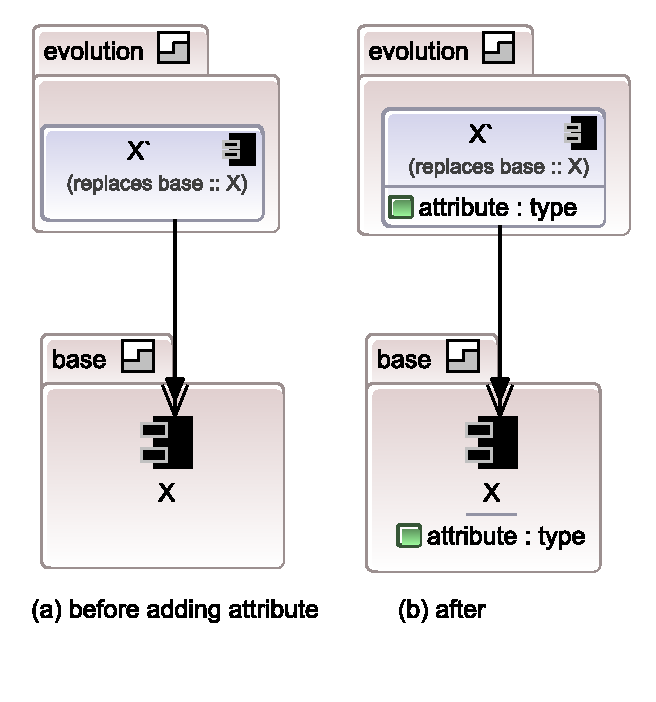
\includegraphics[width=0.5\columnwidth]{images/live-base}
\par\end{centering}

\protect\caption{\label{fig:Adding-an-attribute}Adding an attribute to a base component}
\end{figure}


This models the concurrent creation of a system or framework and the
closely developed first extension of that system. This simultaneous
and synergistic development between a framework and its initial client
is a vital part of exploring and modeling a reusable system.

The Java dependency management system Maven handles temporary mutability
using snapshot dependencies with a suffix of -SNAPSHOT \cite{Varanasi2014,Raemaekers2014}{]}.


\subsubsection*{Implementation mappings}

As the architecture evolves we also may wish to adjust and create
mappings to implementation constructs. Any approach should therefore
also handle these mappings.

The mapping from Evolve component to implementation class is a standard
constituent of each leaf component and hence can be evolved as part
of the same approach. This allows the mappings to be controlled and
evolved in a consistent way with the rest of the architecture.


\subsubsection*{Works without source code}

Following on from this, the source code of a system should not necessarily
be required to evolve that system - in many situations adjusting the
implementation mappings instead will suffice. This approach offers
several benefits. In the first instance, this allows a level of evolution
without being exposed to the complexity of the full source code (as
per plugin systems). Also, the code may not be available for commercial
or licensing reasons.

In Evolve, if the architectural description of a system is available
then adjusting the architectural definitions and implementation mappings
is sufficient to achieve any required evolution. The work required
to achieve this may vary depending on the granularity of the components
being replaced.


\section{Related Work}

We discuss related work from a number of separate directions. Firstly,
we observe that Evolve overlaps with other architectural approaches
to CM. This neatly leads to a comparison of our approach with textual,
distributed CM systems.

We then compare Evolve to extensible systems which provide a limited
form of evolution in order to allow new features to be added to a
base platform without destroying the original architecture. Finally
we compare and contrast our approach to an aspect-oriented architectural
view.


\subsection{Architecture Description Languages}

It has long been recognized that components form a convenient and
powerful unit of software design, composition and reuse \cite{McIlroy1968}.
ADLs build on this foundation to describe the structure of a system
as a connected set of components. An important advance was the composite
component concept whereby a wiring up of component instances itself
forms a new component, thereby enabling a hierarchical approach to
system construction \cite{Kramer2000}.

Some ADLs permit structural inheritance where a new component is defined
in terms of structural changes to a parent \cite{Selic1994,Selic1994a,Barros1996}.
This is related to the concept of object-oriented inheritance in that
it allows changes from a set of parent component to be used to create
a new entity. This increases reusability by allowing us to define
a new set of components in terms of structural addition or deletion
from parents - effectively a limited form of evolution.

However, this only allows us to define new components in terms of
older ones - existing components cannot be altered. This poses a dilemma
- as we build up our architecture as a set of composite components,
which themselves are made up of instances of other composite components
and so on, we form a potentially deep compositional hierarchy. Structural
inheritance only allows us to adjust the topmost level of any hierarchy
as we create a new component. As this hierarchy gets deeper, we are
effectively ``burying'' architecture under compositional layers,
making evolution of the lower layers difficult to achieve.

As such, ADLs with structural inheritance do not fully support unconstrained
architectural change. Depending on whether multiple inheritance and
conflict resolution is allowed, correcting defects after merging branches
may not be supported. There is no intrinsic support for distributed
and disconnected development concepts.

Evolve's key contribution is to supplement structural inheritance
with replacement, and to precisely define the way that the two constructs
interact. Replacement allows us to globally substitute the definition
of a component, and combined with resemblance (structural inheritance)
this allows the incremental evolution of any component. Using this
we can deeply alter existing compositional hierarchies at any level
and resolve any conflicts that occur when branches of the same architecture
are merged.


\subsection{Architecturally Aware Configuration Management Systems}

MAE \cite{Roshandel2004,Hoek2001} is a powerful, centralized CM system
that works with architectural deltas rather than textual deltas. This
permits the explicit evolution and merging of architectural configurations
at the level of architectural concepts, thereby satisfying many of
the properties outlined in section \ref{sub:Essential-Properties-of}.

MAE is already a version control system, hence it cannot easily be
used with conventional CM systems


\subsection{Distributed Configuration Management Systems}

Distributed textual CM systems allow each developer to have a full
or partial copy of the repository on their machine, allowing for operation
even if not connected to a designated ``central'' repository. A
commit is represented as an atomic change set, which has zero, one
or two possible parents. A newly created changeset starting from scratch
has no parent, a linear evolution of a base has one change set, and
a merge has two change sets. Mercurial is a well known example of
this approach \cite{O'Sullivan2009}.

Each changeset is identified by a UUID and the parent/child dependency
relationship is represented by UUID pairs. This allows changesets
to be exported from one repository into another, guaranteeing that
dependency order will be preserved.

Evolve shares a number of concepts with these systems. A stratum is
conceptually related to a changeset, though the deltas are architectural
rather than textual. Also, a stratum may have many parents reflecting
that it is a design as well as a change construct. UUIDs are used
for identification allowing the export and import between repositories.
Unlike changesets, however, non-released strata are not constrained
by rule to be immutable\footnote{By convention an imported stratum is marked as read-only, as it is
generally not owned by the importer.}, and if changes are made to a base stratum they propagate to dependent
strata as per TEMPORARY\_IMMUTABILITY. As such, Mercurial does not
support this property.

Textual CM systems also violate many other of the required and desired
properties for an architectural approach because they work with text
deltas rather than architectural deltas.


\subsection{Extensibility Architectures}

Eclipse uses a plugin-based architecture to allow the system to be
extended for additional features \cite{Gamma2003,Delap2006}. Each
plugin has a version number where the minor digits are used to represent
evolution which does not break existing interfaces, and the major
digits represent breaking change. Plugins also declare dependencies
on other plugins. Through introducing new versions of plugins, an
evolved system can be produced with any extensions required. In this
way, plugins act like change sets in a CM system or strata in Evolve,
and are similar to modules.

However, plugins are not hierarchical meaning that if the source code
is not available and the plugin must be replaced for evolution then
even a small required change can result in significant work. This
highlights an architectural limitation of the approach - plugins form
both the unit of ownership and the unit of replacement. This makes
architectural change at the correct level of abstraction difficult.
It also makes evolution difficult without source code.

Furthermore, although the model ensures that much structural conflict
is avoided, it is not possible to detect conflicts between plugin
combinations in any automated way.


\subsection{Product Lines}

Easel \cite{Hendrickson2007} is a product-line architectural approach
that builds on the ArchStudio toolset \cite{Dashofy2007}. Although
it is not a CM system per se, it is related in that it allows change
sets to be applied against an architecture expressed as components
and connectors. Change sets can be associated to features, and these
can be combined to form variants in the product line. UUIDs are used
to identify change sets and individual architectural entities.

As such, Easel is conceptually similar to the Evolve approach with
a number of similar features. It supports many of the required and
desired properties. It differs, however, from our approach in that
it does not unify modeling concepts (structural inheritance) with
evolution, leading to a less powerful merging approach. Easel change
sets are not hierarchical, which means it is not always possible to
make the change at the appropriate level of abstraction. The delta
primitives are ADD and DELETE and not REPLACE, causing unnecessary
loss of identity when replacement is required and leading to extraneous
merge issues.

AHEAD is a compositional approach to product lines \cite{Batory2006,Batory2003a}.
It introduces constants, which are analogous to a baseline architecture,
and functions which refine constants and can be concatenated to form
an equation. The order of concatenation is important as some forms
of refinement involve overriding parts of other artifacts. 

Mapped onto Java, a constant is a set of class definitions, and a
function contains both class definitions and refinements of classes
consisting of field and method additions and method overrides.

Although AHEAD deals with classes typically rather than architectural
constructs, it can be applied to components via the adoption of conventions.
It is possible, however, to introduce functions that when combined
cause conflict with no possible resolution other than revisiting the
functions and rewriting the equation.


\subsection{Difference-Based Modules}

MixJuice adds a module system to Java, where modules describe the
difference between the base and evolved application \cite{Ichisugi2002,Ichisugi2002a}.
Modules can override classes in the base, allowing unplanned changes
to be catered for. In this sense they are similar to Mercurial change
sets or Evolve strata.

Because it utilizes the Java class model rather than component structures,
MixJuice is not fully compliant with a hierarchical architectural
approach. Some changes cannot be expressed, and merge conflicts which
cannot be corrected via method override can not be resolved.


\subsection{Architectural Aspects}

Aspects have been proposed as a way to evolve an architecture. TranSAT
allows architectural concerns to be specified as aspects \cite{Barais2004}.
These aspects are ``woven'' into a base architecture to evolve it
allowing additional, possibly cross-cutting features to be added in
a modular way.

Each aspect can modify the underlying architectural structure of the
base using a small language where join points are specified declaratively
as a set of structural and behavioral matches. The set of remaking
instructions are similar to those specified in \cite{Magee1996},
and via removal an aspect can remove as well as add functionality.

Like other aspect approaches, this system suffers from a relatively
weaker secondary axis (aspects) that is separate from the primary
axis (base architecture). Further, aspects do not always combine well
and resultant conflicts cannot always be rectified \cite{Ossher2001}.

Evolution in Evolve can be used in place of aspects in most situations.
A stratum can weave additional concerns into a base architecture by
placing parts between existing connected parts in base components.
We must, however, explicitly quantify the join points, as opposed
to using the lexical quantification mechanisms of conventional aspect-orientation
\cite{Filman2000}. As described in the e language, which uses related
evolution primitives to allow verification scripts to be evolved,
this forms a perfectly workable aspect substitute \cite{Vax2007}.


\section{\label{sec:Conclusions-and-Further}Conclusions and Further Work}

The incremental evolution of any software system is inevitable as
it is adjusted over time to deal with improvements and changes in
functionality and requirements. These changes are currently typically
captured at the level of textual differences between releases at a
granular and non-architectural level in configuration management systems.
This leads to a set of challenges and limitations in tying back these
changes to an architectural description, particularly in a distributed
development setting. We have captured these issues as a set of interesting
properties of an architectural approach to the problem.

These properties cover the ability to make any changes at an architectural
level, and later combine these changes if the architectures have diverged
between independent branches. They cover the link between architecture
and implementation, the relationship between system modeling and evolution
and how we capture change relative to other approaches in a distributed
development setting.

Our contribution is address evolution in the above context by supplementing
a hierarchical ADL with three additional concepts. The first is \emph{resemblance},
which is a form of structural inheritance that allows new components
to be defined in terms of structural change to existing components.
This leads naturally to the idea of combining related sets of definitions
into module structures called \emph{stratum}, which express dependencies
on other strata, allowing us to layer a system and express development
ownership of parts of that system. Stratum form the natural unit of
sharing in a distributed setting.

Finally, we add the \emph{replacement} concept to allow global substitution
of a component, within the scope of the stratum that the replacing
component is owned by. Combined with resemblance, this gives us the
ability to incrementally evolve any part of the architecture, such
that the view of the architecture from existing stratum is not affected.
We can therefore capture the gradual evolution of a system in a set
of stratum, which themselves can be shared in a distributed development
setting. Conflict resolution between merged architectures is handled
by the same constructs. In essence, we allow evolution of a system
to be packaged up in a stratum which depends on the original system
stratum. The description of change to a system is packaged up as an
additional stratum.

In applying our approach to a mature system (c.f. \ref{sec:Applicability-to-Mature})
we found that we could gradually decompose an existing code base into
architectural components over time, allowing the evolution to drive
the granular decomposition of the architecture. In other words, as
the system was evolved the architecture became more explicit and fine-grained
leading to a symbiotic relationship between change and architectural
explication.

The analysis of existing extensibility approaches showed that extensibility
is effectively a limited and constrained form of evolution, which
occurs in a distributed development setting of many parties. Therefore,
the same concepts which we use to allow architectural evolution can
also be applied, leading to an advanced approach to extensible systems.
This gives far more flexibility to make changes and later combine
and rectify any divergence than existing approaches such as plugin
architectures.

In applying the approach we have found a number of characteristics
and limitations. In particular, the effort required to evolve a system
depends on how finely grained the architectural decomposition is already.
If we need to replace a component to adjust a small part of its functionality,
and the component is large and monolithic then the architectural change
will not be proportionate to the change in functionality required.
This is tempered by the previously mentioned positive relationship
between evolution and gradual architectural decomposition we found
when evolving a mature system.

Further, our approach so far has been purely limited to structural
concerns. Clearly, behavioral conflict is still possible in a structurally
well-formed system that has been merged from a number of branches.
We plan to address this in further work by allowing a behavioral description
\cite{Magee1999} to be attached to the structural definition of each
(possibly evolved) component. We will then check the system against
a number of goals to ensure that the changes have not affected the
behavioral integrity of the system.

We have built a mature toolset around our approach, including a modeling
tool Evolve which supports the Backbone ADL. This toolset supports
all aspects of the approach allowing the architecture and deltas to
be viewed graphically or textually \cite{McVeigh2015,McVeigh2011}.
A key issue is that components and constituents are identified by
globally unique identifiers allowing us to remove the ambiguity involved
when trying to reconcile diverged branches with human readable names
only. As we have shown, a graphical approach is able to hide the UUIDs,
presenting the human readable names for presentation thereby delivering
the benefits of both.


\section*{Appendix}

Formal Specification
\begin{lyxcode}
{\footnotesize{}open~util/relation}{\footnotesize \par}

{\footnotesize{}fact~Facts~\{}{\footnotesize \par}

{\footnotesize{}~~//~no~strata~cycles}{\footnotesize \par}

{\footnotesize{}~~all~s:~Stratum~|~s~not~in~s.\textasciicircum{}dependson}{\footnotesize \par}

{\footnotesize{}~~//~visibility}{\footnotesize \par}

{\footnotesize{}~~all~e:~Element~|}{\footnotesize \par}

{\footnotesize{}~~~~let~res~=~e.resembles,~rep~=~e.replaces~|}{\footnotesize \par}

{\footnotesize{}~~~~~~res.home~in~e.home.{*}dependson~and}{\footnotesize \par}

{\footnotesize{}~~~~~~rep.home~in~e.home.\textasciicircum{}dependson~and~e~not~in~res}{\footnotesize \par}

{\footnotesize{}~~all~s:~Stratum,~e:~Element~\{}{\footnotesize \par}

{\footnotesize{}~~~~e.home~not~in~s.{*}dependson~=>~\{}{\footnotesize \par}

{\footnotesize{}~~~~~~//~not~necessary,~but~makes~debugging~easier}{\footnotesize \par}

{\footnotesize{}~~~~~~no~s.eresembles{[}e{]}~and~no~s.edeltas{[}e{]}}{\footnotesize \par}

{\footnotesize{}~~~~~~and~no~s.full{[}e{]}}{\footnotesize \par}

{\footnotesize{}~~~~\}}{\footnotesize \par}

{\footnotesize{}~~~~else}{\footnotesize \par}

{\footnotesize{}~~~~\{}{\footnotesize \par}

{\footnotesize{}~~~~~~//~topmost}{\footnotesize \par}

{\footnotesize{}~~~~~~let~reps~=~replaces.e~\&~s.elements~|}{\footnotesize \par}

{\footnotesize{}~~~~~~~~some~reps~=>~s.topmost{[}e{]}~=~reps}{\footnotesize \par}

{\footnotesize{}~~~~~~~~~~else}{\footnotesize \par}

{\footnotesize{}~~~~~~~~e.home~=~s~=>~s.topmost{[}e{]}~=~e}{\footnotesize \par}

{\footnotesize{}~~~~~~~~~~else}{\footnotesize \par}

{\footnotesize{}~~~~~~~~s.topmost{[}e{]}~=~s.dependson.topmost{[}e{]}}{\footnotesize \par}

{\footnotesize{}~~~~~~//~expanded~resembles}{\footnotesize \par}

{\footnotesize{}~~~~~~let~joint~=~e.resembles~\&~e.replaces,}{\footnotesize \par}

{\footnotesize{}~~~~~~~~rest~=~e.resembles~-~joint~|}{\footnotesize \par}

{\footnotesize{}~~~~~~~~~~s.eresembles{[}e{]}~=}{\footnotesize \par}

{\footnotesize{}~~~~~~~~~~~~e.home.dependson.topmost{[}joint{]}}{\footnotesize \par}

{\footnotesize{}~~~~~~~~~~~~+~s.topmost{[}rest{]}}{\footnotesize \par}

{\footnotesize{}~~~~~~//~application~of~deltas}{\footnotesize \par}

{\footnotesize{}~~~~~~let~lower~=~s.eresembles{[}e{]},}{\footnotesize \par}

{\footnotesize{}~~~~~~~~me~=~s.edeltas{[}e{]}}{\footnotesize \par}

{\footnotesize{}~~~~~~\{}{\footnotesize \par}

{\footnotesize{}~~~~~~~~me.add~=~s.edeltas{[}lower{]}.add~+~e.deltas.add}{\footnotesize \par}

{\footnotesize{}~~~~~~~~me.delete~=~s.edeltas{[}lower{]}.delete}{\footnotesize \par}

{\footnotesize{}~~~~~~~~~~+~e.deltas.delete}{\footnotesize \par}

{\footnotesize{}~~~~~~~~me.replace~=~s.edeltas{[}lower{]}.replace}{\footnotesize \par}

{\footnotesize{}~~~~~~~~~~++~e.deltas.replace}{\footnotesize \par}

{\footnotesize{}~~~~~~\}}{\footnotesize \par}

{\footnotesize{}~~~~~~//~final~structure}{\footnotesize \par}

{\footnotesize{}~~~~~~let~tops~=~s.topmost{[}e{]},~me~=~s.edeltas{[}tops{]}~|}{\footnotesize \par}

{\footnotesize{}~~~~~~~~some~e.replaces~=>~no~s.full{[}e{]}}{\footnotesize \par}

{\footnotesize{}~~~~~~~~~~else}{\footnotesize \par}

{\footnotesize{}~~~~~~~~s.full{[}e{]}~=}{\footnotesize \par}

{\footnotesize{}~~~~~~~~~~\{~a,~b:~me.add~|~a~=~b~\}}{\footnotesize \par}

{\footnotesize{}~~~~~~~~~~++~me.replace}{\footnotesize \par}

{\footnotesize{}~~~~~~~~~~-~\{~d:~me.delete,~allds:~Constituent~\}}{\footnotesize \par}

{\footnotesize{}~~~~\}}{\footnotesize \par}

{\footnotesize{}~~\}}{\footnotesize \par}

{\footnotesize{}\}}{\footnotesize \par}

{\footnotesize{}pred~branch{[}a,~b:~Stratum{]}~\{}{\footnotesize \par}

{\footnotesize{}~~let~alla~=~a.{*}dependson,~allb~=~b.{*}dependson~|}{\footnotesize \par}

{\footnotesize{}~~~~a~not~in~allb~and~b~not~in~alla}{\footnotesize \par}

{\footnotesize{}~~~~and~some~alla~\&~allb}{\footnotesize \par}

{\footnotesize{}\}}{\footnotesize \par}

{\footnotesize{}pred~conflict{[}perspective:~Stratum,~e:~Element{]}~\{}{\footnotesize \par}

{\footnotesize{}~~not~functional{[}~perspective.full{[}e{]},~Element~{]}}{\footnotesize \par}

{\footnotesize{}\}}{\footnotesize \par}

{\footnotesize{}sig~Stratum~\{}{\footnotesize \par}

{\footnotesize{}~~name:~lone~String,}{\footnotesize \par}

{\footnotesize{}~~dependson:~set~Stratum,}{\footnotesize \par}

{\footnotesize{}~~elements:~set~Element,}{\footnotesize \par}

{\footnotesize{}~~topmost:~Element~->~Element,}{\footnotesize \par}

{\footnotesize{}~~eresembles:~Element~->~Element,}{\footnotesize \par}

{\footnotesize{}~~edeltas:~Element~->~lone~Deltas,}{\footnotesize \par}

{\footnotesize{}~~full:~Element~->~Constituent~->~Constituent}{\footnotesize \par}

{\footnotesize{}\}}{\footnotesize \par}

{\footnotesize{}\{~elements~=~home.this~\}}{\footnotesize \par}

{\footnotesize{}sig~Element~\{}{\footnotesize \par}

{\footnotesize{}~~name:~lone~String,}{\footnotesize \par}

{\footnotesize{}~~home:~Stratum,}{\footnotesize \par}

{\footnotesize{}~~resembles:~set~Element,}{\footnotesize \par}

{\footnotesize{}~~replaces:~lone~Element,}{\footnotesize \par}

{\footnotesize{}~~deltas:~lone~Deltas}{\footnotesize \par}

{\footnotesize{}\}}{\footnotesize \par}

{\footnotesize{}\{}{\footnotesize \par}

{\footnotesize{}~~let~others~=~Element.@deltas~-~deltas~|}{\footnotesize \par}

{\footnotesize{}~~~~no~deltas.add~\&~others.add~and}{\footnotesize \par}

{\footnotesize{}~~~~no~deltas.replace{[}Constituent{]}}{\footnotesize \par}

{\footnotesize{}~~~~\&~others.replace{[}Constituent{]}}{\footnotesize \par}

{\footnotesize{}\}}{\footnotesize \par}

{\footnotesize{}sig~Deltas}{\footnotesize \par}

{\footnotesize{}\{}{\footnotesize \par}

{\footnotesize{}~~add,~delete:~set~Constituent,}{\footnotesize \par}

{\footnotesize{}~~replace:~Constituent~->~Constituent}{\footnotesize \par}

{\footnotesize{}\}}{\footnotesize \par}

{\footnotesize{}sig~Constituent~\{~name:~lone~String,~parent:~Deltas~\}}{\footnotesize \par}
\end{lyxcode}
To generate the example from figure \ref{fig:A-variant-of}, we used
the following test case.
\begin{lyxcode}
{\footnotesize{}pred~show()~\{}{\footnotesize \par}

{\footnotesize{}~~some~disj~b,~x,~y,~z,~m:~Stratum~\{}{\footnotesize \par}

{\footnotesize{}~~~~no~b.dependson}{\footnotesize \par}

{\footnotesize{}~~~~x.dependson~=~b~and~y.dependson~=~b}{\footnotesize \par}

{\footnotesize{}~~~~z.dependson~=~b}{\footnotesize \par}

{\footnotesize{}~~~~m.dependson~=~x~+~y~+~z}{\footnotesize \par}

{\footnotesize{}~~~~x.name~=~\textquotedbl{}MultiLaneBridge\textquotedbl{}}{\footnotesize \par}

{\footnotesize{}~~~~b.name~=~\textquotedbl{}SingleLangeBridge\textquotedbl{}}{\footnotesize \par}

{\footnotesize{}~~~~y.name~=~\textquotedbl{}EvolvedA\textquotedbl{}~and~m.name~=~\textquotedbl{}Merged\textquotedbl{}}{\footnotesize \par}

{\footnotesize{}~~~~z.name~=~\textquotedbl{}EvolvedB\textquotedbl{}}{\footnotesize \par}

{\footnotesize{}~~~~some~disj~eb,~ex,~ey,~ez:~Element~\{}{\footnotesize \par}

{\footnotesize{}~~~~~~eb.name~=~\textquotedbl{}SLB\textquotedbl{}}{\footnotesize \par}

{\footnotesize{}~~~~~~ex.name~=~\textquotedbl{}MULTISLB\textquotedbl{}}{\footnotesize \par}

{\footnotesize{}~~~~~~ey.name~=~\textquotedbl{}SLBa\textquoteright \textquotedbl{}}{\footnotesize \par}

{\footnotesize{}~~~~~~ez.name~=~\textquotedbl{}SLBb\textquoteright \textquotedbl{}}{\footnotesize \par}

{\footnotesize{}~~~~~~eb.home~=~b~and~ex.home~=~x}{\footnotesize \par}

{\footnotesize{}~~~~~~ey.home~=~y~and~ez.home~=~z}{\footnotesize \par}

{\footnotesize{}~~~~~~no~ex.replaces~and~ex.resembles~=~eb}{\footnotesize \par}

{\footnotesize{}~~~~~~ey.replaces~=~eb~and~ey.resembles~=~eb}{\footnotesize \par}

{\footnotesize{}~~~~~~ez.replaces~=~eb~and~ez.resembles~=~eb}{\footnotesize \par}

{\footnotesize{}~~~~~~no~eb.(replaces~+~resembles)}{\footnotesize \par}

{\footnotesize{}~~~~~~some~c1,~c2,~c3,~c4,~c5:~Constituent~\{}{\footnotesize \par}

{\footnotesize{}~~~~~~~~c1.name~=~\textquotedbl{}c1\textquotedbl{}~and~c2.name~=~\textquotedbl{}c2\textquotedbl{}}{\footnotesize \par}

{\footnotesize{}~~~~~~~~c3.name~=~\textquotedbl{}c3\textquotedbl{}~and~c4.name~=~\textquotedbl{}c4\textquotedbl{}}{\footnotesize \par}

{\footnotesize{}~~~~~~~~c5.name~=~\textquotedbl{}c5\textquotedbl{}}{\footnotesize \par}

{\footnotesize{}~~~~~~~~let~db~=~eb.deltas~|}{\footnotesize \par}

{\footnotesize{}~~~~~~~~~~db.add~=~c1~+~c2~and~no~db.delete}{\footnotesize \par}

{\footnotesize{}~~~~~~~~~~and~no~db.replace}{\footnotesize \par}

{\footnotesize{}~~~~~~~~let~dx~=~ex.deltas~|}{\footnotesize \par}

{\footnotesize{}~~~~~~~~~~dx.add~=~c4~and~no~dx.delete}{\footnotesize \par}

{\footnotesize{}~~~~~~~~~~and~no~dx.replace}{\footnotesize \par}

{\footnotesize{}~~~~~~~~let~dy~=~ey.deltas~|}{\footnotesize \par}

{\footnotesize{}~~~~~~~~~~no~dy.add~and~dy.delete~=~c2}{\footnotesize \par}

{\footnotesize{}~~~~~~~~~~and~dy.replace~=~c1~->~c3}{\footnotesize \par}

{\footnotesize{}~~~~~~~~let~dz~=~ez.deltas~|}{\footnotesize \par}

{\footnotesize{}~~~~~~~~~~dz.add~=~c5~and~no~dz.delete}{\footnotesize \par}

{\footnotesize{}~~~~~~~~~~and~no~dz.replace}{\footnotesize \par}

{\footnotesize{}~~~~~~\}\}\}\}}{\footnotesize \par}

{\footnotesize{}run~show~for~8~but}{\footnotesize \par}

{\footnotesize{}5~Stratum,~4~Element,~25~Deltas,~5~Constituent}{\footnotesize \par}
\end{lyxcode}
\bibliographystyle{spbasic}
\bibliography{\string"/Users/andrew/Personal/Repositories/evolve/Academic Work/read papers/references\string"}

\end{document}
